%%%%%%%%%%%%%%%%%%%%%%%%%%%%%%%%%%%%%%%%%%%%%%%%%%%%%%%%%%%%%%%%%%%%%%%%
%Desarrollo de un juego para Nintendo DS | Trabajo de Fin de Grado
% Escuela Politécnica Superior de la Universidad de Alicante
% Realizado por: Carla Maciá Díez
% Contacto: carlamd1997@hotmail.com / cmd23@alu.ua.es
%%%%%%%%%%%%%%%%%%%%%%%%%%%%%%%%%%%%%%%%%%%%%%%%%%%%%%%%%%%%%%%%%%%%%%%%

\def\OptimizaTikZ{1}
%%%%%%%%%%%%%%%%%%%%%%%%%%%%%%%%%%%%%%%%%%%%%%%%%%%%%%%%%%%%%%%%%%%%%%%%
% Plantilla TFG/TFM
% Escuela Politécnica Superior de la Universidad de Alicante
% Realizado por: Jose Manuel Requena Plens
% Contacto: info@jmrplens.com / Telegram:@jmrplens
%%%%%%%%%%%%%%%%%%%%%%%%%%%%%%%%%%%%%%%%%%%%%%%%%%%%%%%%%%%%%%%%%%%%%%%%

%%%%%%%%%%%%%%%%%%%%%%%%
% FORMATO DEL DOCUMENTO
%%%%%%%%%%%%%%%%%%%%%%%%
% scrbook es la clase de documento
% Si se desea que no haya página en blanco entre capítulos añadir "openany" en los parámetros de la clase. Sino siempre los capítulos empezarán en página impar.
\documentclass[a4paper,11pt,titlepage]{scrbook}
\KOMAoption{toc}{bib,chapterentryfill} % Opciones del índice
\usepackage{scrhack} % Previene algunos errores
% Paquete de formato para scrbook. Con marcas, linea-separador superior e inferior
\usepackage[automark,headsepline,footsepline]{scrlayer-scrpage}
\clearpairofpagestyles		% Borra los estilos por defecto
%%
% Formato y contenido de la información de cabecera y pie de página
%%
% Información de capítulo en cabecera e interno
\ihead{{\color{gray30}\scshape\small\headmark}}	
% Número de página en cabecera y externo
\ohead{\normalfont\pagemark} 
% Número de página en pie de página y externo. Sólo en páginas sin cabecera
\ofoot[\normalfont\pagemark]{}
%% 		
% Edición del contenido de las distintas partes de la cabecera
%%
\renewcommand{\chaptermark}[1]{\markboth{#1}{}} % Capítulo (Solo texto)
\renewcommand{\sectionmark}[1]{\markright{\thesection. #1}} % Sección (Número y texto)
\setkomafont{pagenumber}{} % Número de página (Sin nada añadido)

% Añade al índice y numera hasta la profundidad 4.
% 1:section,2:subsection,3:subsubsection,4:paragraph
\setcounter{tocdepth}{4}
\setcounter{secnumdepth}{4}
% Muestra una regla para comprobar el formato de las páginas
%\usepackage[type=upperleft,showframe,marklength=8mm]{fgruler}
% MÁRGENES DE LAS PÁGINAS
\usepackage[
  inner	=	3.0cm, % Margen interior
  outer	=	2.5cm, % Margen exterior
  top	=	2.5cm, % Margen superior
  bottom=	2.5cm, % Margen inferior
  includeheadfoot, % Incluye cabecera y pie de página en los márgenes
]{geometry}
% Valor de interlineado
\renewcommand{\baselinestretch}{1.0} % 1 línea de interlineado
% Para poder generar páginas horizontales
\usepackage{lscape}
% Ancho de la zona para comentarios en el margen. (modificado para todonotes)
\setlength{\marginparwidth}{1.9cm}

%%%%%%%%%%%%%%%%%%%%%%%%
% BIBLIOGRAFÍA
%%%%%%%%%%%%%%%%%%%%%%%%
\usepackage{apacite} % NORMA APA
\usepackage{natbib}
\usepackage{breakcites}

%%%%%%%%%%%%%%%%%%%%%%%%
% DOCUMENTO EN ESPAÑOL
%%%%%%%%%%%%%%%%%%%%%%%%
\usepackage[base]{babel}
\usepackage{polyglossia}
\setdefaultlanguage{spanish}

\addto\captionsspanish{%
	\renewcommand{\listtablename}{Índice de tablas} 
	\renewcommand{\tablename}{Tabla}
	\renewcommand{\lstlistingname}{Código}
	\renewcommand{\lstlistlistingname}{Índice de \lstlistingname s}
	\renewcommand{\glossaryname}{Glosario}
	\renewcommand{\acronymname}{Acrónimos}
	\renewcommand{\bibname}{Bibliografía}%
}

%%%%%%%%%%%%%%%%%%%%%%%% 
% COLORES
%%%%%%%%%%%%%%%%%%%%%%%% 
% Biblioteca de colores
\usepackage{color}
\usepackage[dvipsnames]{xcolor}
% Otros colores definidos por el usuario
\definecolor{gray97}{gray}{.97}
\definecolor{gray75}{gray}{.75}
\definecolor{gray45}{gray}{.45}
\definecolor{gray30}{gray}{.30}
\definecolor{negro}{RGB}{0,0,0}
\definecolor{blanco}{RGB}{255,255,255}
\definecolor{dkgreen}{rgb}{0,.6,0}
\definecolor{dkblue}{rgb}{0,0,.6}
\definecolor{dkyellow}{cmyk}{0,0,.8,.3}
\definecolor{gray}{rgb}{0.5,0.5,0.5}
\definecolor{mauve}{rgb}{0.58,0,0.82}
\definecolor{deepblue}{rgb}{0,0,0.5}
\definecolor{deepred}{rgb}{0.6,0,0}
\definecolor{deepgreen}{rgb}{0,0.5,0}
\definecolor{MyDarkGreen}{rgb}{0.0,0.4,0.0}
\definecolor{bluekeywords}{rgb}{0.13,0.13,1}
\definecolor{greencomments}{rgb}{0,0.5,0}
\definecolor{redstrings}{rgb}{0.9,0,0}

%%%%%%%%%%%%%%%%%%%%%%%%
% TABLAS
%%%%%%%%%%%%%%%%%%%%%%%%
% Paquetes para tablas
\usepackage{longtable,booktabs,array,multirow,multicol,tabularx,ragged2e,array}
% Nuevos tipos de columna para tabla, se pueden utilizar como por ejemplo C{3cm} en la definición de columnas de la función tabular
\newcolumntype{L}[1]{>{\raggedright\let\newline\\\arraybackslash\hspace{0pt}}m{#1}}
\newcolumntype{C}[1]{>{\centering\let\newline\\\arraybackslash\hspace{0pt}}m{#1}}
\newcolumntype{R}[1]{>{\raggedleft\let\newline\\\arraybackslash\hspace{0pt}}m{#1}}

%%%%%%%%%%%%%%%%%%%%%%%% 
% GRAFICAS y DIAGRAMAS 
%%%%%%%%%%%%%%%%%%%%%%%% 
% Paquete para todo tipo de gráficas, diagramas, modificación de imágenes, etc
\usepackage{tikz,tikzpagenodes}
\usetikzlibrary{tikzmark,calc,shapes.geometric,arrows,backgrounds,shadings,shapes.arrows,shapes.symbols,shadows,positioning,fit,automata,patterns,intersections}
\usepackage{pgfplots}
\pgfplotsset{colormap/jet}
\pgfplotsset{compat=newest} % Compatibilidad
\usepgfplotslibrary{patchplots,groupplots,fillbetween,polar}
\usepackage{pgfplotstable}
% Guardar las figuras realizadas con Tikz y Pgf en una carpeta externa
% para agilizar el procesado y tenerlas para utilizarlas en otros
% documentos
\if\OptimizaTikZ 1
\usepgfplotslibrary{external}
\tikzexternalize[prefix=archivos/figuras-procesadas/] % Ruta
\tikzset{%
    external/system call ={xelatex -enable-write18 -halt-on-error -interaction=batchmode -jobname "\image" "\texsource"},
}
\fi

% Estilos para elementos graficos
% Cajas y cajas de texto
\tikzstyle{Caja1} = [green,very thick,rounded corners,fill=white, fill opacity=0.5]
\tikzstyle{Texto1} = [fill=white,thick,shape=circle,draw=black,inner sep=2pt,font=\sffamily,text=black]
\tikzstyle{Texto2} = [fill=white,thick,shape=rectangle,draw=black,inner sep=2pt,font=\sffamily,text=black]
\tikzstyle{Texto3} = [fill=white,thick,shape=circle,draw=black,inner sep=2pt,font=\sffamily,text=black]
% Cuadros de diagrama
\tikzstyle{rectvioleta} = [rectangle, rounded corners, text centered, draw=black, fill=blue!10]
\tikzstyle{rectnaranja} = [rectangle, minimum width=2cm, minimum height=1cm, text centered, draw=black, fill=orange!10]
\tikzstyle{romborosa} = [diamond, aspect=3, minimum width=3cm, minimum height=1cm, text centered, draw=black, fill=red!10]
\tikzstyle{rectverde} = [rectangle, minimum width=2cm, minimum height=1cm, text centered, draw=black, fill=green!10]
\tikzstyle{rectamarillo} = [rectangle, rounded corners, minimum width=2cm, minimum height=1cm, text centered, draw=black, fill=yellow!10]
% Flechas
\tikzstyle{arrow} = [thick,->,>=stealth]

%%%%%%%%%%%%%%%%%%%%%%%% 
% FIGURAS, TABLAS, ETC 
%%%%%%%%%%%%%%%%%%%%%%%% 
\usepackage{subcaption} % Para poder realizar subfiguras
\usepackage{caption} % Para aumentar las opciones de diseño
% Nombres de figuras, tablas, etc, en negrita la numeración, todo con letra small
\captionsetup{labelfont={bf,small},textfont=small}
% Paquete para modificar los espacios arriba y abajo de una figura o tabla
\usepackage{setspace}
% Define el espacio tanto arriba como abajo de las figuras, tablas
\setlength{\intextsep}{5mm}
% Para ajustar tamaños de texto de toda una tabla o grafica
% Uso: {\scalefont{0.8} \begin{...} \end{...} }
\usepackage{scalefnt}
% Redefine las tablas y figuras para eliminar el '.' entre la numeración y el texto
\renewcommand*{\figureformat}{\figurename~\thefigure}
\renewcommand*{\tableformat}{\tablename~\thetable}

%%%%%%%%%%%%%%%%%%%%%%%% 
% TEXTO
%%%%%%%%%%%%%%%%%%%%%%%%
% Paquete para poder modificar las fuente de texto
\usepackage{xltxtra}
% Cualquier tamaño de texto. Uso: {\fontsize{100pt}{120pt}\selectfont tutexto}
\usepackage{anyfontsize}
% Para modificar parametros del texto.
\usepackage{setspace}
% Paquete para posicionar bloques de texto
\usepackage{textpos}
% Paquete para realizar cajas de texto. 
% Uso: \begin{mdframed}[linecolor=red!100!black] tutexto \end{mdframed}
\usepackage{framed,mdframed}
% Para subrayar. Uso: \hlc[tucolor]{tutexto}
\newcommand{\hlc}[2][yellow]{ {\sethlcolor{#1} \hl{#2}} }

%%%%%%%%%%%%%%%%%%%%%%%% 
% OTROS
%%%%%%%%%%%%%%%%%%%%%%%%
% Para hacer una pagina horizontal. Uso: \begin{landscape} xxxx \end{lanscape}
\usepackage{lscape} 
% Para incluir paginas PDF. Uso:
% \includepdf[pages={1}]{tuarchivo.pdf}
\usepackage{pdfpages}
% Para introducir url's con formato. Uso: \url{http://www.google.es}
\usepackage{url}
% Amplia muchas funciones graficas de latex
\usepackage{graphicx}
% Paquete que añade el hipervinculo en referencias dentro del documento, indice, etc
% Se define sin bordes alrededor. Uso: \ref{tulabel}
\usepackage[pdfborder={000}]{hyperref}
\usepackage{float}
\usepackage{placeins}
\usepackage{afterpage}
\usepackage{verbatim}
% Paquete para condicionales avanzados
\usepackage{xstring,xifthen}
% Paquete para realizar calculos en el código
\usepackage{calc}
% Para rotar tablas o figuras o su contenido
\usepackage{rotating} 
% Para incluir comentarios en el texto. El parámetro 'disable' oculta todas las notas.
% USO: \todo{tutexto}
\usepackage[textsize=tiny,spanish,shadow,textwidth=2cm]{todonotes}
%\reversemarginpar % Descomentar si se quiere todos los comentarios en el mismo lado
% Desactiva la exportación de los ToDo y Missingfigures como figuras
\if\OptimizaTikZ 1
\makeatletter
\renewcommand{\todo}[2][]{\tikzexternaldisable\@todo[#1]{#2}\tikzexternalenable}
\makeatother
\usepackage{letltxmacro}
\LetLtxMacro{\oldmissingfigure}{\missingfigure}
\makeatletter
\renewcommand{\missingfigure}[2][]{\tikzexternaldisable\oldmissingfigure[{#1}]{#2}\tikzexternalenable}
\makeatother
\fi

%%%%%%%%%%%%%%%%%%%%%%%% 
% GLOSARIOS
%%%%%%%%%%%%%%%%%%%%%%%%
\usepackage[acronym,nonumberlist,toc]{glossaries}
\usepackage{glossary-superragged}
\newglossarystyle{modsuper}{%
  \setglossarystyle{super}%
  \renewcommand{\glsgroupskip}{}
}
\renewcommand{\glsnamefont}[1]{\textbf{#1}}


%%%%%%%%%%%%%%%%%%%%%%%% 
% COMANDOS AÑADIDOS
%%%%%%%%%%%%%%%%%%%%%%%%
% Para mostrar la fecha actual (mes año) con \Hoy
\newcommand{\MES}{%
  \ifcase\month% 0
    \or Enero% 1
    \or Febrero% 2
    \or Marzo% 3
    \or Abril% 4
    \or Mayo% 5
    \or Junio% 6
    \or Julio% 7
    \or Agosto% 8
    \or Septiembre% 9
    \or Octubre% 10
    \or Noviembre% 11
    \or Diciembre% 12
  \fi}
\newcommand{\ANYO}{\number\year}
\newcommand{\Hoy}{\MES\ \ANYO}

%%%%%%%%%%%%%%%%%%%%%%%% 
% MATEMÁTICAS
%%%%%%%%%%%%%%%%%%%%%%%%
\usepackage{mathtools,amsthm,amsfonts,amssymb,bm,mathrsfs,nicefrac,upgreek,bigints} 
% Comando para añadir información de variables a las ecuaciones
% Uso: \begin{condiciones}[donde:] ....... \end{condiciones}
\newenvironment{condiciones}[1][2]
  {%
   #1\tabularx{\textwidth-\widthof{#1}}[t]{
     >{$}l<{$} @{}>{${}}c<{{}$}@{} >{\raggedright\arraybackslash}X
   }%
  }
  {\endtabularx\\[\belowdisplayskip]}

%%%%%
% PARÁMETROS DE FORMATO DE CODIGOS
%%%%%
% Puedes editar los formatos para ajustarlos a tu gusto
%%%%%%%%%%%%%%%%%%%%%%%%%%%%%%%%%%%%%%%%%%%%%%%%%%%%%%%%%%%%%%%%%%%%%%%%
% Plantilla TFG/TFM
% Escuela Politécnica Superior de la Universidad de Alicante
% Realizado por: Jose Manuel Requena Plens
% Contacto: info@jmrplens.com / Telegram:@jmrplens
%%%%%%%%%%%%%%%%%%%%%%%%%%%%%%%%%%%%%%%%%%%%%%%%%%%%%%%%%%%%%%%%%%%%%%%%


%%%%%%%%%%%%%%%%%%%%%%%% 
% CÓDIGO. CONFIGURACIÓN. En el siguiente bloque están los estilos.
%%%%%%%%%%%%%%%%%%%%%%%%
% Paquete para mostrar código de matlab. En caja y lineas numeradas
\usepackage[framed,numbered]{matlab-prettifier}
% Paquete mostrar código de programación de distintos lenguajes
\usepackage{listings}
\lstset{ inputencoding=utf8,
extendedchars=true,
frame=single, % Caja donde se ubica el código
backgroundcolor=\color{gray97}, % Color del fondo de la caja
rulesepcolor=\color{black},
boxpos=c,
abovecaptionskip=-4pt,
aboveskip=12pt,
belowskip=0pt,
lineskip=0pt,
framerule=0pt,
framextopmargin=4pt,
framexbottommargin=4pt,
framexleftmargin=11pt,
framexrightmargin=0pt,
linewidth=\linewidth,
xleftmargin=\parindent,
framesep=0pt,
rulesep=.4pt,
stringstyle=\ttfamily,
showstringspaces = false,
showspaces = false,
showtabs = false,
columns=fullflexible,
basicstyle=\small\ttfamily,
commentstyle=\color{gray45},
keywordstyle=\bfseries,
tabsize=4,
numbers=left,
numbersep=1pt,
numberstyle=\tiny\ttfamily\color{gray75},
numberfirstline = false,
breaklines=true,
postbreak=\mbox{\textcolor{red}{$\hookrightarrow$}\space}, % Flecha al saltar de linea
prebreak=\mbox{\textcolor{red}{$\hookleftarrow$}\space}, % Flecha al saltar de linea
literate=
  {á}{{\'a}}1 {é}{{\'e}}1 {í}{{\'i}}1 {ó}{{\'o}}1 {ú}{{\'u}}1
  {Á}{{\'A}}1 {É}{{\'E}}1 {Í}{{\'I}}1 {Ó}{{\'O}}1 {Ú}{{\'U}}1
  {à}{{\`a}}1 {è}{{\`e}}1 {ì}{{\`i}}1 {ò}{{\`o}}1 {ù}{{\`u}}1
  {À}{{\`A}}1 {È}{{\'E}}1 {Ì}{{\`I}}1 {Ò}{{\`O}}1 {Ù}{{\`U}}1
  {ä}{{\"a}}1 {ë}{{\"e}}1 {ï}{{\"i}}1 {ö}{{\"o}}1 {ü}{{\"u}}1
  {Ä}{{\"A}}1 {Ë}{{\"E}}1 {Ï}{{\"I}}1 {Ö}{{\"O}}1 {Ü}{{\"U}}1
  {â}{{\^a}}1 {ê}{{\^e}}1 {î}{{\^i}}1 {ô}{{\^o}}1 {û}{{\^u}}1
  {Â}{{\^A}}1 {Ê}{{\^E}}1 {Î}{{\^I}}1 {Ô}{{\^O}}1 {Û}{{\^U}}1
  {œ}{{\oe}}1 {Œ}{{\OE}}1 {æ}{{\ae}}1 {Æ}{{\AE}}1 {ß}{{\ss}}1
  {ű}{{\H{u}}}1 {Ű}{{\H{U}}}1 {ő}{{\H{o}}}1 {Ő}{{\H{O}}}1
  {ç}{{\c c}}1 {Ç}{{\c C}}1 {ø}{{\o}}1 {å}{{\r a}}1 {Å}{{\r A}}1
  {€}{{\euro}}1 {£}{{\pounds}}1 {«}{{\guillemotleft}}1
  {»}{{\guillemotright}}1 {ñ}{{\~n}}1 {Ñ}{{\~N}}1 {¿}{{?`}}1,
  }

% Intenta no dividir los códigos en diferentes paginas si es posible
\lstnewenvironment{listing}[1][]
   {\lstset{#1}\pagebreak[0]}{\pagebreak[0]}

% Formato de títulos de los códigos
\DeclareCaptionFont{white}{\color{white}}
\DeclareCaptionFormat{listing}{\colorbox{gray}{\parbox{\textwidth - 2\fboxsep}{#1#2#3}}}
\captionsetup[lstlisting]{format=listing,labelfont=white,textfont=white,font= scriptsize}


%%%%%%%%%%%%%%%%%%%%%%%% 
% CÓDIGO. ESTILOS. Ajústalos a tu gusto
%%%%%%%%%%%%%%%%%%%%%%%%
\lstdefinestyle{Consola}
	{
	basicstyle=\scriptsize\bf\ttfamily,
	}
   
\lstdefinestyle{C}
	{
	basicstyle=\scriptsize,
	language=C,
	}
\lstdefinestyle{C-color}
	{
  	breaklines=true,
  	language=C,
  	basicstyle=\scriptsize,
  	keywordstyle=\bfseries\color{green!40!black},
  	commentstyle=\itshape\color{purple!40!black},
  	identifierstyle=\color{blue},
  	stringstyle=\color{orange},
    }
\lstdefinestyle{CSharp}
	{
	basicstyle=\scriptsize
	language=[Sharp]C,
	escapeinside={(*@}{@*)},
	keywordstyle=\bfseries,
	}
\lstdefinestyle{CSharp-color}
	{
	basicstyle=\scriptsize
	language=[Sharp]C,
	escapeinside={(*@}{@*)},
	commentstyle=\color{greencomments},
	keywordstyle=\color{bluekeywords}\bfseries,
	stringstyle=\color{redstrings},
	}
\lstdefinestyle{C++}
	{
	basicstyle=\scriptsize,
	language=C++,
 	}
 	
\lstdefinestyle{C++-color}
	{
  	breaklines=true,
  	language=C++,
  	basicstyle=\scriptsize,
  	keywordstyle=\bfseries\color{green!40!black},
  	commentstyle=\itshape\color{purple!40!black},
  	identifierstyle=\color{blue},
  	stringstyle=\color{orange},
    }
    
\lstdefinestyle{PHP}
	{
	basicstyle=\scriptsize,
	language=PHP,
	}
	
\lstdefinestyle{PHP-color}
	{
	basicstyle=\scriptsize,
	language=PHP,
	keywordstyle    = \color{dkblue},
  	stringstyle     = \color{red},
  	identifierstyle = \color{dkgreen},
  	commentstyle    = \color{gray},
  	emph            =[1]{php},
  	emphstyle       =[1]\color{black},
  	emph            =[2]{if,and,or,else},
  	emphstyle       =[2]\color{dkyellow}
  }
  
\lstdefinestyle{Matlab}
	{
	basicstyle=\scriptsize,
	language=Matlab,
	numberstyle=\tiny\ttfamily\color{gray75},
	}
	
\lstdefinestyle{Matlab-color}
	{
	style = Matlab-editor,
	basicstyle=\scriptsize,
	numberstyle=\tiny\ttfamily\color{gray75},
	}
	
\lstdefinestyle{Latex}
	{
	language=[LaTeX]{Tex},
    basicstyle=\scriptsize,
    literate={\$}{{{\bfseries\$}}}1,
    alsoletter={\\,*,\&},
    emph =[1]{\\begin,\\end,\\caption,\\label,\\centering,\\FloatBarrier,
              \\lstinputlisting,\\scalefont,\\addplot,\\input,
              \\legend,\\item,\\subitem,\\includegraphics,\\textwidth,
              \\section,\\subsection,\\subsubsection,\\paragraph,
              \\cite,\\citet,\\citep,\\gls,\\bibliographystyle,\\url,
              \\citet*,\\citep*,\\todo,\\missingfigure,\\footnote},
  	emphstyle =[1]\bfseries,
  	emph = [2]{equation,subequations,eqnarray,figure,subfigure,
  			   condiciones,flalign,tikzpicture,axis,lstlisting,
  			   itemize,description
  			   },
  	emphstyle =[2]\bfseries,
    numbers=none,
	}
	
\lstdefinestyle{Latex-color}
	{
	language=[LaTeX]{Tex},
    basicstyle=\scriptsize,
    commentstyle=\color{dkgreen},
    identifierstyle=\color{black},
    literate={\$}{{{\bfseries\color{Dandelion}\$}}}1, % Colorea el simbolo dollar
    alsoletter={\\,*,\&},
    emph =[1]{\\begin,\\end,\\caption,\\label,\\centering,\\FloatBarrier,
              \\lstinputlisting,\\scalefont,\\addplot,\\input,
              \\legend,\\item,\\subitem,\\includegraphics,\\textwidth,
              \\section,\\subsection,\\subsubsection,\\paragraph,
              \\cite,\\citet,\\citep,\\gls,\\bibliographystyle,\\url,
              \\citet*,\\citep*,\\todo,\\missingfigure,\\footnote},
  	emphstyle =[1]\bfseries\color{RoyalBlue},
  	emph = [2]{equation,subequations,eqnarray,figure,subfigure,
  			   condiciones,flalign,tikzpicture,axis,lstlisting,
  			   itemize,description
  			   },
  	emphstyle =[2]\bfseries,
    numbers=none,
	}
\lstdefinestyle{Java}
{
	basicstyle=\scriptsize,
	language=Java,
}

\lstdefinestyle{Java-color}
{
	basicstyle=\scriptsize,
	language=Java,
  	keywordstyle=\color{blue},
  	commentstyle=\color{dkgreen},
  	stringstyle=\color{mauve},
}
\lstdefinestyle{Python}
{
	language=Python,
	basicstyle=\scriptsize,
	otherkeywords={self},  
	keywordstyle=\bfseries,     
	emphstyle=\bfseries,    
	emph={MyClass,__init__},         
}

\lstdefinestyle{Python-color}
{
	language=Python,
	basicstyle=\scriptsize,
	otherkeywords={self},          
	keywordstyle=\bfseries\color{deepblue},
	emph={MyClass,__init__},         
	emphstyle=\bfseries\color{deepred},    
	stringstyle=\color{deepgreen},
}
\lstdefinestyle{R}
{
	language=R,                     
  	basicstyle=\scriptsize,
  	keywordstyle=\bfseries, 
}
\lstdefinestyle{R-color}
{
	language=R,                     
  	basicstyle=\scriptsize,
  	keywordstyle=\bfseries\color{RoyalBlue}, 
  	commentstyle=\color{YellowGreen},
  	stringstyle=\color{ForestGreen}  
}


%%%%%
% DEFINICION DE CONCEPTOS
%%%%
% Uso ejemplo: \begin{ejemplo} tucontenido \end{ejemplo} 
\newtheorem{teorema}{Teorema}[chapter]
\newtheorem{ejemplo}{Ejemplo}[chapter]
\newtheorem{definicion}{Definición}[chapter]



\newcommand{\titulo}{Touch \& Brush}
\newcommand{\subtitulo}{Videojuego para Nintendo DS y manual de desarrollo}
\newcommand{\miNombre}{Carla Macia Diez}
\newcommand{\miEmail}{cmd23@alu.ua.es}
\newcommand{\miTutor}{Francisco José Gallego Durán}
\newcommand{\departamentoTutor}{Departamento de Ciencia de la Computación e Inteligencia Artificial}
\newcommand{\miFacultad}{Escuela Politécnica Superior}
\newcommand{\miFacultadCorto}{EPS UA}
\newcommand{\miUniversidad}{\protect{Universidad de Alicante}}
\newcommand{\miUbicacion}{Alicante}

\def\IDtitulo{5} 

%%%%%%%%%%%%%%%%%%%%%%%%%%%%%%%%%%%%%%%%%%%%%%%%%%%%%%%%%%%%%%%%%%%%%%%%
% Plantilla TFG/TFM
% Escuela Politécnica Superior de la Universidad de Alicante
% Realizado por: Jose Manuel Requena Plens
% Contacto: info@jmrplens.com / Telegram:@jmrplens
%%%%%%%%%%%%%%%%%%%%%%%%%%%%%%%%%%%%%%%%%%%%%%%%%%%%%%%%%%%%%%%%%%%%%%%%

%%%%%%%%%%%%%%%%%%%%%%%% 
% COLORES DE GRADOS.
% Si el color de la titulación ha cambiado, modifícalo en las lineas siguientes.
%%%%%%%%%%%%%%%%%%%%%%%%
% Grados
\definecolor{teleco}{RGB}{32,2,116}			% Teleco
\definecolor{civil}{RGB}{201,56,140}			% Civil
\definecolor{quimica}{RGB}{41,199,255}		% Química
\definecolor{informatica}{RGB}{0,128,255}	% Informatica
\definecolor{multimedia}{RGB}{239,206,53}	% Multimedia
\definecolor{arquitecnica}{RGB}{0,179,148}	% Arquitectura técnica
\definecolor{arquitectura}{RGB}{181,0,0}		% Arquitectura
\definecolor{robotica}{RGB}{0,128,255}		% Robótica
% Másteres
\definecolor{masterteleco}{RGB}{32,2,116}	% Teleco
\definecolor{caminos}{RGB}{201,56,140}		% Caminos, Canales y Puertos
\definecolor{gestedif}{RGB}{50,120,50}		% Gestión Edificación
\definecolor{desweb}{RGB}{250,43,22}			% Desarrollo Web
\definecolor{mataguaterre}{RGB}{210,250,50}	% Materiales, Agua, Terreno
\definecolor{masterinfor}{RGB}{0,128,255}	% Informática
\definecolor{autorobo}{RGB}{83,145,201}		% Automática y Robótica
\definecolor{prevencion}{RGB}{0,100,0}		% Prevención Riesgos
\definecolor{gestionagua}{RGB}{7,138,197}	% Gestión Agua
\definecolor{moviles}{RGB}{121,11,21}		% Aplicaciones Móviles
\definecolor{masterquimica}{RGB}{41,199,255}	% Aplicaciones Móviles

% Logotipos comunes de todas las titulaciones
\newcommand{\logoFacultad}{include/logos-universidad/LogoEPSNegro}
\newcommand{\logoUniversidad}{include/logos-universidad/LogoUANegro}
\newcommand{\logoUniversidadPortada}{include/logos-universidad/LogoUABlanco}

% Colores generales
\definecolor{negro}{RGB}{0,0,0}
\definecolor{blanco}{RGB}{255,255,255}
%%%%%%%%%%%%%%%%%%%%%%%% 
% CONDICIONALES. SEGUN LA ID ELEGIDA EN EL .TEX PRINCIPAL
% Según el ID seleccionado en TFG_EPS_UA.tex se configurará el nombre de la titulación, logotipos y color.
% Si tu titulación no esta correctamente definida cambia las imágenes que se definen para tu titulación en las lineas de abajo
% Si deseas añadir mas titulaciones ve al final de este archivo
%%%%%%%%%%%%%%%%%%%%%%%%
% Grados
	\if\IDtitulo 1 % Teleco
		% Logos
		\newcommand{\logoFacultadPortada}{include/logos-universidad/LogoEPSBlanco}
		\newcommand{\logoGradoPortada}{include/logos-titulaciones/LogoTelecoBlanco}
		\newcommand{\logoGrado}{include/logos-titulaciones/LogoTelecoNegro}
		% Texto
		\newcommand{\miGrado}{Grado en Ingeniería en Sonido e Imagen en Telecomunicación}
		\newcommand{\tipotrabajo}{Trabajo Fin de Grado}
		% Color
		\newcommand{\colorgrado}{teleco}
		\newcommand{\colortexto}{blanco}
	\else \if\IDtitulo 2 % Civil
		\newcommand{\logoFacultadPortada}{include/logos-universidad/LogoEPSBlanco}
		\newcommand{\logoGradoPortada}{include/logos-titulaciones/LogoCivilBlanco}
		\newcommand{\logoGrado}{include/logos-titulaciones/LogoCivilNegro}
		% Texto
		\newcommand{\miGrado}{Grado en Ingeniería Civil}
		\newcommand{\tipotrabajo}{Trabajo Fin de Grado}
		% Color
		\newcommand{\colorgrado}{civil}
		\newcommand{\colortexto}{blanco}
	\else \if\IDtitulo 3 % Quimica
		% Logos
		\newcommand{\logoFacultadPortada}{include/logos-universidad/LogoEPSNegro}
		\newcommand{\logoGradoPortada}{include/logos-titulaciones/LogoQuimicaNegro}
		\newcommand{\logoGrado}{include/logos-titulaciones/LogoQuimicaNegro}
		% Texto
		\newcommand{\miGrado}{Grado en Ingeniería Química}
		\newcommand{\tipotrabajo}{Trabajo Fin de Grado}
		% Color
		\newcommand{\colorgrado}{quimica}
		\newcommand{\colortexto}{negro}
	\else \if\IDtitulo 4 % Informatica
		% Logos
		\newcommand{\logoFacultadPortada}{include/logos-universidad/LogoEPSBlanco}
		\newcommand{\logoGradoPortada}{include/logos-titulaciones/LogoInformaticaBlanco}
		\newcommand{\logoGrado}{include/logos-titulaciones/LogoInformaticaNegro}
		% Texto
		\newcommand{\miGrado}{Grado en Ingeniería Informática}
		\newcommand{\tipotrabajo}{Trabajo Fin de Grado}
		% Color
		\newcommand{\colorgrado}{informatica}
		\newcommand{\colortexto}{blanco}
	\else \if\IDtitulo 5 % Multimedia
		% Logos
		\newcommand{\logoFacultadPortada}{include/logos-universidad/LogoEPSNegro}
		\newcommand{\logoGradoPortada}{include/logos-titulaciones/LogoMultimediaNegro}
		\newcommand{\logoGrado}{include/logos-titulaciones/LogoMultimediaNegro}
		% Texto
		\newcommand{\miGrado}{Grado en Ingeniería Multimedia}
		\newcommand{\tipotrabajo}{Trabajo Fin de Grado}
		% Color
		\newcommand{\colorgrado}{multimedia}
		\newcommand{\colortexto}{negro}
	\else \if\IDtitulo 6 % Arquitectura Tecnica
		% Logos
		\newcommand{\logoFacultadPortada}{include/logos-universidad/LogoEPSBlanco}
		\newcommand{\logoGradoPortada}{include/logos-titulaciones/LogoArqTecnicaBlanco}
		\newcommand{\logoGrado}{include/logos-titulaciones/LogoArqTecnicaNegro}
		% Texto
		\newcommand{\miGrado}{Grado en Arquitectura Técnica}
		\newcommand{\tipotrabajo}{Trabajo Fin de Grado}
		% Color
		\newcommand{\colorgrado}{arquitecnica}
		\newcommand{\colortexto}{blanco}
	\else \if\IDtitulo 7 % Arquitectura
		% Logos
		\newcommand{\logoFacultadPortada}{include/logos-universidad/LogoEPSBlanco}
		\newcommand{\logoGradoPortada}{include/logos-titulaciones/LogoArquitecturaBlanco}
		\newcommand{\logoGrado}{include/logos-titulaciones/LogoArquitecturaNegro}
		% Texto
		\newcommand{\miGrado}{Grado en Arquitectura}
		\newcommand{\tipotrabajo}{Trabajo Fin de Grado}
		% Color
		\newcommand{\colorgrado}{arquitectura}
		\newcommand{\colortexto}{blanco}
	\else \if\IDtitulo 8 % Robotica
		% Logos
		\newcommand{\logoFacultadPortada}{include/logos-universidad/LogoEPSBlanco}
		\newcommand{\logoGradoPortada}{include/logos-titulaciones/LogoInformaticaBlanco}
		\newcommand{\logoGrado}{include/logos-titulaciones/LogoInformaticaNegro}
		% Texto
		\newcommand{\miGrado}{Grado en Ingeniería Robótica}
		\newcommand{\tipotrabajo}{Trabajo Fin de Grado}
		% Color
		\newcommand{\colorgrado}{robotica}
		\newcommand{\colortexto}{blanco}
% Másteres
	\else \if\IDtitulo A % Teleco
		% Logos
		\newcommand{\logoFacultadPortada}{include/logos-universidad/LogoEPSBlanco}
		\newcommand{\logoGradoPortada}{include/logos-titulaciones/LogoTelecoBlanco}
		\newcommand{\logoGrado}{include/logos-titulaciones/LogoTelecoNegro}
		% Texto
		\newcommand{\miGrado}{Máster Universitario en Ingeniería en Telecomunicación}
		\newcommand{\tipotrabajo}{Trabajo Fin de Máster}
		% Color
		\newcommand{\colorgrado}{masterteleco}
		\newcommand{\colortexto}{blanco}
	\else \if\IDtitulo B % Caminos, Canales y puertos
		% Logos
		\newcommand{\logoFacultadPortada}{include/logos-universidad/LogoEPSBlanco}
		\newcommand{\logoGradoPortada}{include/logos-titulaciones/LogoCivilBlanco}
		\newcommand{\logoGrado}{include/logos-titulaciones/LogoCivilNegro}
		% Texto
		\newcommand{\miGrado}{Máster Universitario en Ingeniería de Caminos, Canales y Puertos}
		\newcommand{\tipotrabajo}{Trabajo Fin de Máster}
		% Color
		\newcommand{\colorgrado}{caminos}
		\newcommand{\colortexto}{blanco}
	\else \if\IDtitulo C % Gestión Edificación
		% Logos
		\newcommand{\logoFacultadPortada}{include/logos-universidad/LogoEPSBlanco}
		\newcommand{\logoGradoPortada}{include/logos-titulaciones/LogoMasterEdificacionBlanco}
		\newcommand{\logoGrado}{include/logos-titulaciones/LogoMasterEdificacionNegro}
		\newcommand{\tipotrabajo}{Trabajo Fin de Máster}
		% Texto
		\newcommand{\miGrado}{Máster Universitario en Gestión de la Edificación}
		% Color
		\newcommand{\colorgrado}{gestedif}
		\newcommand{\colortexto}{blanco}
	\else \if\IDtitulo D % Desarrollo web
		% Logos
		\newcommand{\logoFacultadPortada}{include/logos-universidad/LogoEPSBlanco}
		\newcommand{\logoGradoPortada}{include/logos-titulaciones/LogoMasterDesarrolloBlanco}
		\newcommand{\logoGrado}{include/logos-titulaciones/LogoMasterDesarrolloNegro}
		% Texto
		\newcommand{\miGrado}{Máster Universitario en Desarrollo de Aplicaciones y Servicios Web}
		\newcommand{\tipotrabajo}{Trabajo Fin de Máster}
		% Color
		\newcommand{\colorgrado}{desweb}
		\newcommand{\colortexto}{blanco}
	\else \if\IDtitulo E % Materiales, Agua, Terreno
		% Logos
		\newcommand{\logoFacultadPortada}{include/logos-universidad/LogoEPSNegro}
		\newcommand{\logoGradoPortada}{include/logos-titulaciones/LogoMasterMaterialesNegro}
		\newcommand{\logoGrado}{include/logos-titulaciones/LogoMasterMaterialesNegro}
		% Texto
		\newcommand{\miGrado}{Máster Universitario en Ingeniería de los Materiales, del Agua y del Terreno}
		\newcommand{\tipotrabajo}{Trabajo Fin de Máster}
		% Color
		\newcommand{\colorgrado}{mataguaterre}
		\newcommand{\colortexto}{negro}
	\else \if\IDtitulo F % Informatica
		% Logos
		\newcommand{\logoFacultadPortada}{include/logos-universidad/LogoEPSBlanco}
		\newcommand{\logoGradoPortada}{include/logos-titulaciones/LogoInformaticaBlanco}
		\newcommand{\logoGrado}{include/logos-titulaciones/LogoInformaticaNegro}
		% Texto
		\newcommand{\miGrado}{Máster Universitario en Ingeniería Informática}
		\newcommand{\tipotrabajo}{Trabajo Fin de Máster}
		% Color
		\newcommand{\colorgrado}{masterinfor}
		\newcommand{\colortexto}{blanco}
	\else \if\IDtitulo G % Automática y Robótica
		% Logos
		\newcommand{\logoFacultadPortada}{include/logos-universidad/LogoEPSBlanco}
		\newcommand{\logoGradoPortada}{include/logos-titulaciones/LogoMasterRoboticaBlanco}
		\newcommand{\logoGrado}{include/logos-titulaciones/LogoMasterRoboticaNegro}
		% Texto
		\newcommand{\miGrado}{Máster Universitario en Automática y Robótica}
		\newcommand{\tipotrabajo}{Trabajo Fin de Máster}
		% Color
		\newcommand{\colorgrado}{autorobo}
		\newcommand{\colortexto}{blanco}
	\else \if\IDtitulo H % Prevención de riesgos laborales
		% Logos
		\newcommand{\logoFacultadPortada}{include/logos-universidad/LogoEPSBlanco}
		\newcommand{\logoGradoPortada}{include/logos-titulaciones/LogoMasterPrevencionBlanco}
		\newcommand{\logoGrado}{include/logos-titulaciones/LogoMasterPrevencionNegro}
		% Texto
		\newcommand{\miGrado}{Máster Universitario en Prevención de Riesgos Laborales}
		\newcommand{\tipotrabajo}{Trabajo Fin de Máster}
		% Color
		\newcommand{\colorgrado}{prevencion}
		\newcommand{\colortexto}{blanco}
	\else \if\IDtitulo I % Gestion Agua
		% Logos
		\newcommand{\logoFacultadPortada}{include/logos-universidad/LogoEPSNegro}
		\newcommand{\logoGradoPortada}{include/logos-titulaciones/LogoMasterAguaNegro}
		\newcommand{\logoGrado}{include/logos-titulaciones/LogoMasterAguaNegro}
		% Texto
		\newcommand{\miGrado}{Máster Universitario en Gestión Sostenible y Tecnologías del Agua}
		\newcommand{\tipotrabajo}{Trabajo Fin de Máster}
		% Color
		\newcommand{\colorgrado}{gestionagua}
		\newcommand{\colortexto}{negro}
	\else \if\IDtitulo J % Aplicaciones Móviles
		% Logos
		\newcommand{\logoFacultadPortada}{include/logos-universidad/LogoEPSBlanco}
		\newcommand{\logoGradoPortada}{include/logos-titulaciones/LogoMasterMovilesBlanco}
		\newcommand{\logoGrado}{include/logos-titulaciones/LogoMasterMovilesNegro}
		% Texto
		\newcommand{\miGrado}{Máster Universitario en Desarrollo de Software para Dispositivos Móviles}
		\newcommand{\tipotrabajo}{Trabajo Fin de Máster}
		% Color
		\newcommand{\colorgrado}{moviles}
		\newcommand{\colortexto}{blanco}
	\else \if\IDtitulo K % Quimica
		% Logos
		\newcommand{\logoFacultadPortada}{include/logos-universidad/LogoEPSNegro}
		\newcommand{\logoGradoPortada}{include/logos-titulaciones/LogoQuimicaNegro}
		\newcommand{\logoGrado}{include/logos-titulaciones/LogoQuimicaNegro}
		% Texto
		\newcommand{\miGrado}{Máster Universitario en Ingeniería Química}
		\newcommand{\tipotrabajo}{Trabajo Fin de Máster}
		% Color
		\newcommand{\colorgrado}{masterquimica}
		\newcommand{\colortexto}{negro}


	\fi \fi \fi \fi \fi \fi \fi \fi \fi \fi \fi \fi \fi \fi \fi \fi \fi \fi \fi
	
%%%%%%%%%%%%%%%%%%%%%%%%%%%%%%%%%%%%%%%%%%%%%%%%%%%%%%%%%%%%%%%%%%%%%%%%	
% ¿COMO AÑADIR MÁS TITULACIONES?
% Para añadir más titulaciones, se debe continuar el el formato de ID -> Titulacion.
% Justo encima de la linea donde hay muchos '\fi' se debe escribir el condicional y el contenido de este tal que:
%
%	\else \if\IDtitulo X % Titulacion con ID=X		
% 		% Logos
%		\newcommand{\logoFacultadPortada}{include/logos-universidad/LogoEPSBlanco}
%		\newcommand{\logoGradoPortada}{include/logos-titulaciones/logotitulacion}
%		\newcommand{\logoGrado}{include/logos-titulaciones/logotitulacion}
%		% Texto
%		\newcommand{\miGrado}{Grado en XXXXXXXX}
%		\newcommand{\tipotrabajo}{Trabajo Fin de XXXX}
%		% Color
%		\newcommand{\colorgrado}{XXXX}
%		\newcommand{\colortexto}{XXX}
%	
% Por último añadir a la linea que tiene muchos '\fi', otro '\fi'. Listo, ya podrás usar la nueva ID con la configuración añadida.
%%%%%%%%%%%%%%%%%%%%%%%%%%%%%%%%%%%%%%%%%%%%%%%%%%%%%%%%%%%%%%%%%%%%%%%%	




 

% Información añadida a las propiedades del archivo PDF.
\hypersetup{
pdfauthor = {\miNombre~(\miEmail)},
pdftitle = {\titulo},
}

\usepackage{graphicx}
\usepackage{amsmath}
\usepackage{hyperref}
\usepackage{amssymb}
\usepackage{verbatim}

%%%%%%%%%%%%%%%%%%%%%%%% 
% INICIO DEL DOCUMENTO
%%%%%%%%%%%%%%%%%%%%%%%%
\begin{document}


% Números romanos hasta el mainmatter.
\frontmatter

% PORTADA
%%%%%%%%%%%%%%%%%%%%%%%%%%%%%%%%%%%%%%%%%%%%%%%%%%%%%%%%%%%%%%%%%%%%%%%%
% Plantilla TFG/TFM
% Escuela Politécnica Superior de la Universidad de Alicante
% Realizado por: Jose Manuel Requena Plens
% Contacto: info@jmrplens.com / Telegram:@jmrplens
%%%%%%%%%%%%%%%%%%%%%%%%%%%%%%%%%%%%%%%%%%%%%%%%%%%%%%%%%%%%%%%%%%%%%%%%

%%%%%%%%%%%%%%%%%%%%%%%%
% PORTADA - no modificar
%%%%%%%%%%%%%%%%%%%%%%%%
% Establece las fuentes de texto de la portada
% Helvetica LS Std Cond. Uso: {\FuenteTitulo tutexto}
\newfontfamily\FuenteTitulo{HelveticaLTStd-Cond}[Path=./include/fuentes/]  
% Helvetica. Uso: {\FuentePortada tutexto}
\newfontfamily\FuentePortada{Helvetica}[Path=./include/fuentes/]  

% Ignora los márgenes establecidos para el documento. Después de la portada en blanco y negro (portada_bn.tex) devuelve los márgenes establecidos en configuracioninicial.tex
\newgeometry{ignoreall,top=2cm,outer=2cm,inner=2cm}

% Tamaño por defecto de la fuente de texto para:
\def\FuenteTamano{55pt}	% Tamaño para el título del trabajo
\def\interlinportada{5.0} % Interlineado por defecto para el título
\def\TamTrabajo{20pt} 	% Tamaño para el tipo de trabajo (grado o máster)
\def\TamTrabajoIn{20pt} 	% Tamaño para el salto de línea después de tipo de trabajo
\def\TamOtros{12pt} 	% Tamaño para datos personales y fecha
\def\TamOtrosIn{1pt} 	% Tamaño para los saltos de línea en la info personal

% Según la longitud del título se determina un tamaño e interlineado para él
\StrLen{\titulo}[\longitudtitulo] % Cuenta los caracteres título
% Comprueba la longitud del título y según sea este determina unos valores nuevos
\ifthenelse{\longitudtitulo > 180}{
\def\FuenteTamano{35pt}		% Si es mayor a 180 caracteres tamaño de fuente 35pt
\def\interlinportada{3.5}} 	% Establece nuevo interlineado
{\ifthenelse{\longitudtitulo > 140}{
\def\FuenteTamano{40pt}		% Si es mayor a 140 caracteres tamaño de fuente 40pt
\def\interlinportada{4.0}} 	% Establece nuevo interlineado
{\ifthenelse{\longitudtitulo > 120}{
\def\FuenteTamano{50pt}		% Si es mayor a 120 caracteres tamaño de fuente 50pt
\def\interlinportada{4.5}} 	% Establece nuevo interlineado
{} % Si no, no modifica el tamaño
} }

\if\OptimizaTikZ 1
\tikzexternaldisable % Desactiva la exportación com figura
\fi 

% Inicio de portada
\begin{titlepage}
% Offset horizontal para toda la portada
\newlength{\centeroffset}
\setlength{\centeroffset}{-0.5\oddsidemargin}
\addtolength{\centeroffset}{0.5\evensidemargin}
\thispagestyle{empty}

% Fondo del color del grado
\pagecolor{\colorgrado}
% Logo de la facultad en la esquina superior derecha
\begin{tikzpicture}[remember picture,overlay]
   \node[anchor=north west,inner sep=0pt] at ($(current page.north west)+(13.65cm,-1.4cm)$)
              {\includegraphics[width=5.3cm]{\logoFacultadPortada}};
\end{tikzpicture}

% Titulo y subtitulo
\hspace{0pt}
\vfill
\hspace{-0.8cm}\begin{tabular}{L{18cm}}
\begin{spacing}{\interlinportada}
{\raggedleft{\FuenteTitulo\fontsize{\FuenteTamano}{110pt}\selectfont\color{\colortexto}\titulo}}
\vspace{-7em}
\end{spacing}
\end{tabular}
\hfill\linebreak\\
\begin{tabular}{lL{12cm}}
\raisebox{-.35\height}{\includegraphics[width=2cm]{\logoGradoPortada}} & \begin{spacing}{1.5}{\raggedleft{\FuentePortada\fontsize{20pt}{40pt}\selectfont\color{\colortexto}\miGrado}} \end{spacing}\\
\end{tabular}
\vspace{2cm}
\vfill
\hspace{0pt}
% Franja negra con logotipo 
\begin{tikzpicture}[overlay, remember picture, inner sep=0pt, outer sep=0pt]
  \fill [black] (current page.south west) rectangle (\paperwidth,\paperheight-26.4cm);
\node[anchor=south west,inner sep=0pt] at ($(current page.south west)+(13.2cm,1.6cm)$)
              {\includegraphics[width=6.2cm]{\logoUniversidadPortada}};
\end{tikzpicture}

% Información personal y fecha
\begin{textblock*}{\textwidth}(0.3cm,-2.35cm)% Ancho - Pos X,PosY
\noindent {\FuentePortada \fontsize{\TamTrabajo}{45pt}\selectfont\color{white}\tipotrabajo}
\\[\TamTrabajoIn] 
{\FuentePortada \fontsize{\TamOtros}{30pt}\selectfont\color{white} Autor:}
\\[\TamOtrosIn]
{\FuentePortada \fontsize{\TamOtros}{50pt}\selectfont\color{white}\miNombre}
\\[\TamOtrosIn]
{\FuentePortada \fontsize{\TamOtros}{30pt}\selectfont\color{white} Tutor/es:}
\\[\TamOtrosIn]
{\FuentePortada \fontsize{\TamOtros}{30pt}\selectfont\color{white}\miTutor}
\\[\TamOtrosIn]
\ifx\miTutorB\undefined \else {\FuentePortada \fontsize{\TamOtros}{30pt}\selectfont\color{white}\miTutorB} \fi
\\[\TamOtrosIn]\\[\TamOtrosIn]		
{\FuentePortada \fontsize{\TamOtros}{30pt}\selectfont\color{white}\Hoy}
\end{textblock*}


\end{titlepage}

\if\OptimizaTikZ 1
\tikzexternalenable % Reactiva la exportación como figura
\fi

\pagecolor{white}






 % Portada Color
%%%%%%%%%%%%%%%%%%%%%%%%%%%%%%%%%%%%%%%%%%%%%%%%%%%%%%%%%%%%%%%%%%%%%%%%
% Plantilla TFG/TFM
% Escuela Politécnica Superior de la Universidad de Alicante
% Realizado por: Jose Manuel Requena Plens
% Contacto: info@jmrplens.com / Telegram:@jmrplens
%%%%%%%%%%%%%%%%%%%%%%%%%%%%%%%%%%%%%%%%%%%%%%%%%%%%%%%%%%%%%%%%%%%%%%%%

\begin{titlepage}

% Márgenes de esta pagina modificados
\newgeometry{ignoreall,top=2cm,bottom=2cm}

% Offset horizontal para toda la portada
\setlength{\centeroffset}{-0.5\oddsidemargin}
\addtolength{\centeroffset}{0.5\evensidemargin}
\thispagestyle{empty}

% Titulo y subtitulo
\noindent\hspace*{\centeroffset}\begin{minipage}{\textwidth}
\centering
\begin{spacing}{1.5}{\huge\bfseries \titulo}\end{spacing}
\noindent\rule[-1ex]{\textwidth}{3pt}\\[3.5ex] % Linea
{\large\bfseries \subtitulo\\[4cm]}
\end{minipage}

% Relleno hasta la zona central
\vspace{2.5cm}

% Zona central. Autor y Tutores
\noindent\hspace*{\centeroffset}
\begin{minipage}{\textwidth}
\centering

\textbf{Autor}\\ {\miNombre}\\[2.5ex]
\textbf{Tutor/es}\\
{\normalsize \miTutor\\
\ifx\departamentoTutor\undefined \else \small\textit \departamentoTutor\\ \fi
\ifx\miTutorB\undefined \else \normalsize \miTutorB\\ \fi
\ifx\departamentoTutorB\undefined \else\small\textit \departamentoTutorB\\[2cm] \fi
}
\end{minipage}

% Relleno hasta la zona de abajo
\vspace*{\fill}

% Zona de abajo
\noindent\hspace*{\centeroffset}
\begin{minipage}{\textwidth}
\centering
\noindent\hspace*{\centeroffset}
\begin{center}
{\includegraphics[width=3cm]{\logoGrado}}\\
{\raggedleft\miGrado}
\end{center}
\vspace*{2em}
\centering
\noindent\hspace*{\centeroffset}
\begin{minipage}[l]{6cm}
\includegraphics[width=5cm]{\logoFacultad}
\end{minipage}
\begin{minipage}[r]{6cm}
\includegraphics[width=5cm]{\logoUniversidad}
\end{minipage}
\\[1cm]
ALICANTE, \Hoy
\end{minipage}


\end{titlepage}

% A partir de aquí aplica los márgenes establecidos en configuracioninicial.tex
\restoregeometry


 % Portada B/N

%%%%% PREAMBULO
% Incluye el .tex que contiene el preámbulo, agradecimientos y dedicatorias.
%%%%%%%%%%%%%%%%%%%%%%%%%%%%%%%%%%%%%%%%%%%%%%%%%%%%%%%%%%%%%%%%%%%%%%%%
%Desarrollo de un juego para Nintendo DS | Trabajo de Fin de Grado
% Escuela Politécnica Superior de la Universidad de Alicante
% Realizado por: Carla Maciá Díez
% Contacto: carlamd1997@hotmail.com / cmd23@alu.ua.es
%%%%%%%%%%%%%%%%%%%%%%%%%%%%%%%%%%%%%%%%%%%%%%%%%%%%%%%%%%%%%%%%%%%%%%%%

\chapter{Resumen}
\textbf{Touch \& Brush} es un videojuego de agilidad mental para la consola \textbf{Nintendo DS}, desarollado en \textbf{C++} y el conjunto de herramientas de \textbf{devkitPro}, basado principalmente en \textbf{Magic Cat Academy} de Google (Doodle de Halloween 2016).

\vspace{0.5cm}

En cada \textbf{nivel}  el jugador deberá vencer a un número de enemigos para poder continuar y estos irán apareciendo alrededor de la pantalla e irán moviéndose hacia el jugador, el cual estará en el centro. Dichos enemigos poseerán un \textbf{patrón} visible que el jugador deberá \textbf{dibujar} correctamente en la pantalla táctil para poder derrotarlos antes de que ellos le alcancen y le quiten vida.

{\let\clearpage\relax\chapter*{Abstract}}
\textbf{Touch \& Brush} is a mental agility video game for the \textbf{Nintendo DS} console, developed in \textbf{C ++} and using \textbf{devkitPro} toolkit, based mainly on Google's \textbf{Magic Cat Academy} (2016 Halloween Doodle).

\vspace{0.5cm}

On each \textbf{level} the player must defeat a number of enemies in order to continue and they will appear around the screen and move towards the player, who will be in the center. These enemies will have a \textbf{pattern} that the player must correctly \textbf{draw} in the touch screen in order to defeat them before they reach  and damage him.


\chapter{Justificación y objetivos}
\thispagestyle{empty}
Desde que comencé el grado en ingeniería multimedia hace ya 5 años he podido participar en el desarrollo de un gran número de proyectos enfocados en los videojuegos que, aunque se traten de simples demos básicas con fines totalmente didácticos, me han servido para darme cuenta de que no solo me apasiona jugar a videojuegos, sino que también adoro crearlos. Es por eso que mi último proyecto como estudiante de este grado no podía ser otro que crear un videojuego para la consola que más horas de diversión me ha brindado en mi infancia: la Nintendo DS.

\vspace{0.5cm}

Este proyecto supone una gran ilusión para mi, pues ser capaz de crear un juego para una plataforma en la que años atrás yo disfrutaba y pasaba horas y horas jugando tanto a sus grandes títulos es un sentimiento que no puedo llegar a expresar con palabras, y que por supuesto, influirá a la hora de perfeccionar cada detalle. Además, para poder desarrollar un juego de una manera correcta debemos \textbf{entender cómo trabaja la máquina} a bajo nivel, así, siempre que cometamos un fallo seremos capaces de localizar el error más rápido y solucionarlo de una forma eficiente. En los ordenadores y consolas modernos esto puede llegar a ser un gran dolor de cabeza para el desarrollador, pues son \textbf{máquinas muy complejas}. Sin embargo, las \textbf{consolas retro}, al tratarse de una versión \textbf{simplificada}, son unas \textbf{excelentes candidatas} para comenzar desarrollando pequeños juegos que nos permitan entender su funcionamiento y que, al fin y al cabo, la base de las máquinas modernas también está ahí.

\vspace{0.5cm}

Por otro lado, la Nintendo DS es una consola con \textit{hardware} específico para el desarrollo de juegos a la que se le puede sacar muchísimo partido y, obviamente, las grandes empresas que antiguamente desarollaban para esta máquina no iban a andar compartiendo el código fuente ni enseñando a terceros. Es por ello que si como fanático deseas introducirte en el mundo del desarrollo para Nintendo DS y buscas información, lo más probable es que pases horas y horas leyendo artículos hechos por personas que han creado manuales con pequeñas demos y ejemplos pero que llevan muchos años sin actualizarse o no terminen de explicar del todo lo que tú esperas. Así pues, espero poder enfocar esta memoria a modo de \textbf{manual} para que le \textbf{sirva a cualquier persona que desee desarrollar para la Nintendo DS.}

\vspace{0.5cm}

Dicho esto, los objetivos a cumplir en la realización de este proyecto son:

\begin{itemize}
   \item \textbf{Analizar la Nintendo DS y entender sus capacidades y limitaciones.}
   \item  \textbf{Analizar librerías y frameworks existentes.}
    \item \textbf{Aprender/Profundizar programación en C++.}
    \item \textbf{Comprender el funcionamiento del hardware.}
     \item  \textbf{Diseñar y desarrollar un videojuego completo.}
     \item \textbf{Realizar la producción física del videojuego en cartucho.}
     \item \textbf{Elaborar un manual de desarrollo referenciable que aúne el conocimiento disponible sobre desarrollo en Nintendo DS.}
\end{itemize}


\cleardoublepage %salta a nueva página impar
\chapter{Agradecimientos}
Antes de nada, he de agradecer a todas las personas que me han ayudado, no solo durante todo el desarrollo de este proyecto, sino también durante toda mi etapa como estudiante de este grado. Ellos han sido gran parte de mi motivación a seguir adelante y mi apoyo en los momentos más difíciles.

\vspace{0.5cm}

En primer lugar gracias a mis padres, por proporcionarme los medios necesarios para poder formarme en un campo que tanto me gusta y por interesarse por éste a pesar de no entender mucho del tema. También, por saber detectar cuándo lo estaba pasando mal e intentar ayudarme al instante, a pesar de que yo sea de pocas palabras en ese aspecto.

\vspace{0.5cm}

A mi pareja y amigos, no solo a los antiguos, también a los que he conocido en el grado y que me han permitido aprender mucho de ellos. Ángel, Leire, Franck, Yaiza, Raquel, Mer, Alberto... con ellos y muchos más he podido compartir gran cantidad de trabajos, \textit{hobbies}, buenos y malos momentos que sin duda espero seguir compartiendo en el futuro.

\vspace{0.5cm}

Y por último, gracias a mi tutor y al profesorado del grado, en especial a los profesores de cuarto curso. Ellos me han ayudado a ver la luz al final del túnel y hacerme creer que puedo dedicarme a esto después de unos primeros años de caos y de estar perdida entre tantas asignaturas distintas. Gracias a su dedicación y esfuerzo los alumnos de multimedia hemos podido disfrutar al máximo nuestros ultimos años de carrera.

\vspace{0.5cm}

A todos y cada uno de vosotros, gracias.

\thispagestyle{empty}



%\cleardoublepage %salta a nueva página impar
%% Aquí va la dedicatoria si la hubiese. Si no, comentar la(s) linea(s) siguientes
%\chapter*{}
%\label{dedicatoria}
%\setlength{\leftmargin}{0.5\textwidth}
%\setlength{\parsep}{0cm}
%\addtolength{\topsep}{0.5cm}
%\begin{flushright}
%\small\em{
%Una pequeña dedicatoria al líder supremo de Corea del Norte.
%%A toda persona que ha pasado por mi vida,
%%sin las cuales no sería la persona que soy hoy.
%}
%\end{flushright}


\cleardoublepage %salta a nueva página impar
 

% Incluye después del archivo anterior el indice y lista de figuras, tablas y códigos.
\tableofcontents	% Índice
\listoffigures		% Índice de figuras
\listoftables		% Índice de tablas
\lstlistoflistings	% Índice de códigos

%%%%%%%%%%%%%%%%%%%%%%%%%%%%%%%%%%%%%%%%%%%%%%%%%%%%%%%%%%%%%%%%%%%%%%%%
%Desarrollo de un juego para Nintendo DS | Trabajo de Fin de Grado
% Escuela Politécnica Superior de la Universidad de Alicante
% Realizado por: Carla Maciá Díez
% Contacto: carlamd1997@hotmail.com / cmd23@alu.ua.es
%%%%%%%%%%%%%%%%%%%%%%%%%%%%%%%%%%%%%%%%%%%%%%%%%%%%%%%%%%%%%%%%%%%%%%%%

\chapter{Terminología}

A  lo largo de este documento se van a utilizar una serie de abreviaturas con el fin de hacer la lectura más amena. Todos estos términos están explicados a continuación.

\begin{itemize}
  \item \textbf{NDS:} Nintendo DS.
  \item \textbf{NDSi:} Nintendo DSi.
  \item \textbf{GBA:} Game Boy Advance.
  \item \textbf{ARM9:} Procesador ARM946E-S de la Nintendo DS.
  \item \textbf{ARM7:} Procesador ARM7TDMI de la Nintendo DS.
  \item \textbf{R4:} Revolution for NDS.
  \item \textbf{RPG:} Role Playing Game o videojuego de rol. 
  \item \textbf{VRAM:} Memoria RAM de vídeo.
  \item \textbf{RAM:} Memoria de Acceso Aleatorio.
  \item \textbf{NPC:} Non Playable Characters, hace referencia a todos los personajes que aparecen en el juego que no son el jugador.
  \item \textbf{HUD:} Head-Up Display, es la información que, por lo general en un videojuego se muestra siempre por pantalla.
  \item \textbf{GRF:} Formato de archivo gráfico usado por Microsoft GraphEdit.
\end{itemize}


% Inicia la numeración habitual.
\mainmatter


%%%%
% CONTENIDO. CAPÍTULOS DEL TRABAJO - Añade o elimina según tus necesidades
%%%%

%%%%%%%%%%%%%%%%%%%%%%%%%%%%%%%%%%%%%%%%%%%%%%%%%%%%%%%%%%%%%%%%%%%%%%%%
% Plantilla TFG/TFM
% Escuela Politécnica Superior de la Universidad de Alicante
% Realizado por: Jose Manuel Requena Plens
% Contacto: info@jmrplens.com / Telegram:@jmrplens
%%%%%%%%%%%%%%%%%%%%%%%%%%%%%%%%%%%%%%%%%%%%%%%%%%%%%%%%%%%%%%%%%%%%%%%%

\chapter{Introducción}

Este proyecto trata sobre el desarrollo de un \textbf{juego para la consola} de Nintendo, \textbf{Nintendo DS} y sus posteriores versiones (hasta la Nintendo DSi XL).

\vspace{0.5cm}

El videojuego, titulado Touch \& Brush, se trata de un juego de categoría \textbf{agilidad mental} y en el cual se progresa por \textbf{niveles}. En cada nivel, aparecerán una serie de \textbf{enemigos} que tendrán un \textbf{patrón específico} e irán a atacar al jugador. Este, si no quiere perder todas sus vidas y por tanto la partida, debe ser más rápido y \textbf{dibujar dichos patrones} en la pantalla táctil para derrotarlos.

\vspace{0.5cm}

Esta es una idea que puede parecer sencilla, pero que a nivel técnico lleva bastante trabajo, no solo por desarrollar todas las \textbf{mecánicas y aspectos visuales} para una consola limitada como es la Nintendo DS, sino también porque el propio proyecto requiere analizar, investigar, e incluso desarrollar un \textbf{algoritmo de reconocimiento de gestos}, para que el juego sea capaz de identificar el trazo del usuario. Y eso no es un trabajo que pueda hacerse en una tarde.

\vspace{0.5cm}

También, requiere trabajo tanto de \textbf{diseño del juego} completo, como \textbf{planificación} del proyecto, y sobre todo la parte de \textbf{documentación}, pues uno de los objetivos es que esta memoria sirva de referencia o manual a cualquiera con una base de programación que quiera desarrollar para NDS. Por ello, debemos plasmar cada concepto y procedimiento de la manera más detallada posible.

\vspace{0.5cm}

Por otro lado, la Nintendo DS, tal y como hemos dicho, se trata de una consola con limitaciones técnicas, es por ello que debemos \textbf{analizarla} previamente así como conocer las diferencias entre sus versiones. Tiene dos procesadores ARM que ejecutan los juegos originales y retrocompatibles, doble pantalla (siendo una de ellas táctil), zonas hardware dedicadas a los gráficos (VRAM, OAM), soporte para sonido estéreo...

\vspace{0.5cm}

Todos y cada uno de esos aspectos los describiremos en los apartados siguientes.























	
%%%%%%%%%%%%%%%%%%%%%%%%%%%%%%%%%%%%%%%%%%%%%%%%%%%%%%%%%%%%%%%%%%%%%%%%%
%Desarrollo de un juego para Nintendo DS | Trabajo de Fin de Grado
% Escuela Politécnica Superior de la Universidad de Alicante
% Realizado por: Carla Maciá Díez
% Contacto: carlamd1997@hotmail.com / cmd23@alu.ua.es
%%%%%%%%%%%%%%%%%%%%%%%%%%%%%%%%%%%%%%%%%%%%%%%%%%%%%%%%%%%%%%%%%%%%%%%%


\chapter{Nintendo DS} 

La \textbf{Nintendo DS} es una videoconsola portátil de la compañía de origen japonés; \textbf{Nintendo}. Creada para suceder a la Game Boy Advance, se lanzó al mercado el \textbf{21 de noviembre de 2004 en Estados Unidos}, retrasándose su fecha de lanzamiento en \textbf{Japón al 2 de diciembre} y en\textbf{ Europa al 5 de marzo del año siguiente} con un \textbf{precio de 149.99€}. La consola original y sus versiones posteriores alcanzaron un total de \textbf{154,90 millones unidades vendidas} en todo el mundo y su videojuego más vendido fue el \textbf{New Super Mario Bros}, con un total de 30,80 millones de copias vendidas.

\vspace{0.5cm}

\begin{figure}[htbp]
\centering
  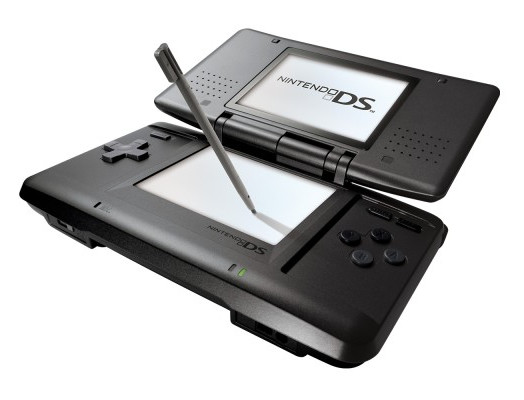
\includegraphics[width=0.4\textwidth]{archivos/nds.jpg}
  \caption{Nintendo DS}
  \textbf{Fuente:} \href{https://www.nintendo.co.uk/Nintendo-DS/Nintendo-DS-Family-Nintendo-UK-s-official-site-Nintendo-DS-Nintendo-DSi-Nintendo-DSi-XL-116380.html}{Nintendo}
  \label{fig:nds1}
\end{figure}

\vspace{0.5cm}

La consola consta de \textbf{ dos pantallas LCD} retroiluminadas con brillo ajustable, siendo una de ellas (la inferior) \textbf{ táctil}, un  \textbf{pad de direcciones},  \textbf{seis botones de acción} (A,B,X,Y, R y L) , \textbf{dos botones de control} (Start y Select) y un \textbf{micrófono}. En su interior posee \textbf{dos procesadores}, un \textbf{ARM946E-S} de 67 MHz que, en general, se encarga de la mayor parte del trabajo ejecutando los \textbf{juegos de NDS} y un \textbf{ARM7TDMI} de 33 MHz, que mueve los juegos de \textbf{GBA} y algunas funciones Wi-Fi. Profundizaremos en ambos procesadores más adelante.

\vspace{0.5cm}

Como curiosidad, las siglas DS significan \textbf{Developer's System} (Sistema de desarrolladores) ya que según la compañía, este sistema ofrece muchas herramientas para que los desarrolladores puedan innovar en sus creaciones. No obstante, también hicieron oficial que estas siglas también hacían referencia a \textbf{Dual Screen}, por su doble pantalla.

\vspace{1cm}

\section{Versiones}

Ahora que conocemos un poco más la Nintendo DS original, es importante que analicemos sus posteriores ediciones ya que nuestro juego debe funcionar en cualquiera de ellas. Debemos conocer qué diferencias significativas existen y tenerlas en cuenta a la hora de desarrollar el juego. Así pues vamos a ir revisando la familia de consolas de Nintendo DS y conociendo sus principales cambios.

\vspace{1cm}

%\subsection{Nintendo DS}

%\begin{figure}[htbp]
%\centering
  %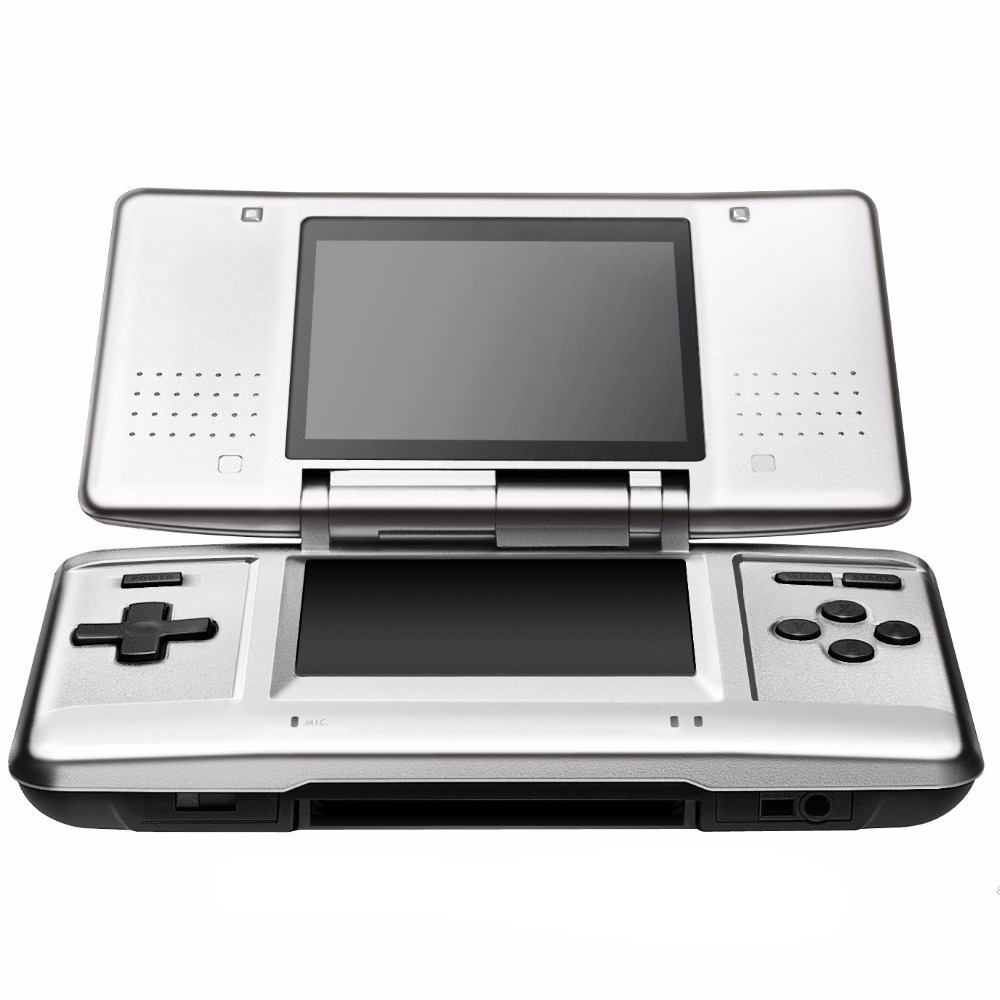
\includegraphics[width=0.3\textwidth]{archivos/nds2.jpg}
 % \caption{Nintendo DS}
  %\label{fig:nds2} %si cambio esto se irá la ref a la *??
%\end{figure}

\subsection{Nintendo DS Lite}

Fue creada en \textbf{2006} por Nintendo, es ligeramente \textbf{más pequeña} que su predecesora e incluía una \textbf{carcasa} más elegante. Algunos \textbf{botones} fueron \textbf{relocalizados} y añadía la función de poder elegir entre \textbf{4 niveles de brillo} a diferencia de la original, que solo podía ajustarse al mínimo o al máximo.

\vspace{0.5cm}

\begin{figure}[htbp]
\centering
  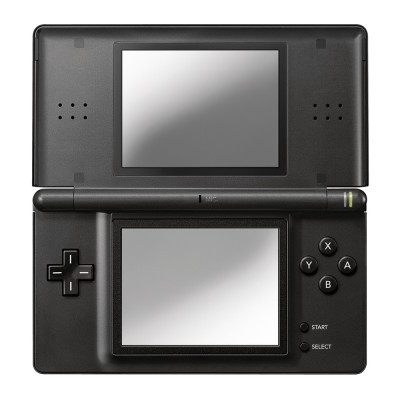
\includegraphics[width=0.3\textwidth]{archivos/ndslite.jpg}
  \caption{Nintendo DS Lite}
    \textbf{Fuente:} \href{https://www.nintendo.co.uk/Nintendo-DS/Nintendo-DS-Family-Nintendo-UK-s-official-site-Nintendo-DS-Nintendo-DSi-Nintendo-DSi-XL-116380.html}{Nintendo}
  \label{fig:ndslite}
\end{figure}

\vspace{1cm}

\subsection{Nintendo DSi}

Salió a la venta a finales de \textbf{2008 en Japón} y en \textbf{2009 en el restro del mundo} y se trata de una \textbf{revisión} del modelo de la Nintendo DS Lite. Si bien mantiene muchas características intactas, hay algunas otras que se deben destacar.

\vspace{0.5cm}

\begin{figure}[htbp]
\centering
  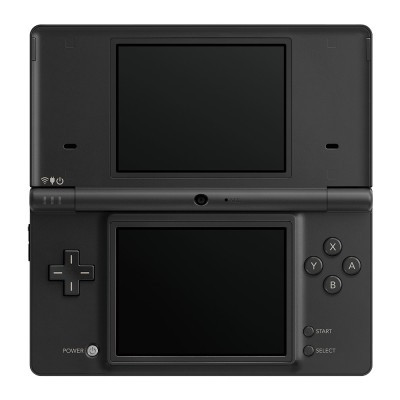
\includegraphics[width=0.3\textwidth]{archivos/ndsi.jpg}
  \caption{Nintendo DSi}
    \textbf{Fuente:} \href{https://www.nintendo.co.uk/Nintendo-DS/Nintendo-DS-Family-Nintendo-UK-s-official-site-Nintendo-DS-Nintendo-DSi-Nintendo-DSi-XL-116380.html}{Nintendo}
  \label{fig:ndsi}
\end{figure}

\vspace{0.5cm}

El primer cambio notable y que a mucha gente no le agradó fue que \textbf{dejaba de ser compatible} con los juegos de \textbf{GBA}, pues ya no poseía ranura para los cartuchos. Introdujeron una \textbf{cámara delantera} y otra \textbf{trasera}, ambas de 0.3 megapíxeles, con las que podías hacer fotos y editarlas mediante un programa llamado \textbf{Cámara DSi} que venía instalado en la consola por defecto.  Poseía también una ranura para \textbf{tarjetas SD}, en las que podías guardar las fotos de la cámara así como los programas o juegos que descargases de la \textbf{Tienda Nintendo DSi}.

\vspace{0.5cm}

Por último, otras mejoras o diferencias frente a sus modelos originales son una \textbf{mejora de la calidad del audio}, \textbf{aumento} de la \textbf{memoria interna y RAM}, el procesador principal \textbf{ARM9} pasó a ser de 133 MHz (\textbf{aumentando su velocidad}), un \textbf{aumento} ligero del \textbf{tamaño de las pantallas} y \textbf{reducción} de la \textbf{duración de la batería} a 16 horas, siendo de 18 horas y media las originales.

\vspace{0.5cm}

El \textbf{menú principal} de la consola es completamente distinto al de la DS original, pasando a ser bastante \textbf{más personalizable} y con una gran variedad de programas, los cuales algunos de ellos se mantenían desde la DS como el \textbf{Picto-Chat} o la \textbf{Descarga DS}.

\vspace{0.5cm}

\begin{figure}[htbp]
\centering
  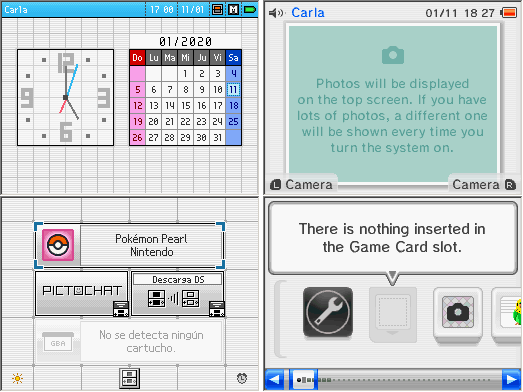
\includegraphics[width=0.6\textwidth]{archivos/nds-ndsi-menu.png}
  \caption{Menú de Nintendo DS (izquierda) frente al de Nintendo DSi (derecha)}
  \label{fig:menu-comparacion} %si cambio esto se irá la ref a la *??
\end{figure}

\vspace{0.5cm}

Fué la primera consola portátil en tener \textbf{bloqueo regional}, no permitiendo que juegos desarrollados en países extranjeros se ejecutasen en la consola si esta era originaria del mismo país.

\vspace{1cm}

\subsection{Nintendo DSi XL}

Se trata de un modelo adicional de NDSi que salió a la venta en \textbf{Japón en 2009}, donde originalmente se bautizó como Nintendo DSi LL, llegando a \textbf{España en 2010} donde pasó a llamarse Nintendo DSi XL.

\vspace{0.5cm}

\begin{figure}[htbp]
\centering
  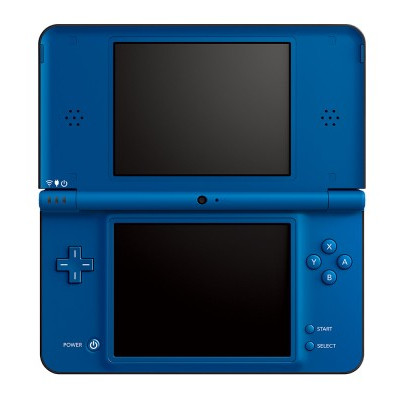
\includegraphics[width=0.3\textwidth]{archivos/ndsixl.jpg}
  \caption{Nintendo DSi XL}
    \textbf{Fuente:} \href{https://www.nintendo.co.uk/Nintendo-DS/Nintendo-DS-Family-Nintendo-UK-s-official-site-Nintendo-DS-Nintendo-DSi-Nintendo-DSi-XL-116380.html}{Nintendo}
  \label{fig:ndsixl} %si cambio esto se irá la ref a la *??
\end{figure}

\vspace{0.5cm}

El principal cambio destacable es el considerable aumento del tamaño de la consola como consecuencia del \textbf{aumento del tamaño de las pantallas} (estas tienen aproximadamente \textbf{una pulgada más} comparadas con la NDSi). En general es una consola perfecta para aquellos que tengan alguna discapacidad visual o les sea difícil o incómodo jugar con las anteriores por su tamaño.

\vspace{1cm}

\section{Especificaciones}

En esta sección vamos a conocer los detalles técnicos de la consola y profundizar en los más interesantes para poder entender qué la compone. Podemos ver a continuación una tabla a modo de resumen.

\vspace{0.5cm}

\begin{table}[htbp]

\centering

\begin{tabular}{|l|l|lll}

\cline{1-2}

\textbf{CPU}                & \begin{tabular}[c]{@{}l@{}}ARM946E-S 32bit RISC CPU\\ ARM7TDMI 32bit RISC CPU\end{tabular} &  &  &  \\ \cline{1-2}

\textbf{Velocidad de reloj} & \begin{tabular}[c]{@{}l@{}}(ARM9) 66MHz\\ (ARM7) 33MHz (16MHz en modo GBA)\end{tabular}    &  &  &  \\ \cline{1-2}

\textbf{RAM}                & 4096KB                                                                                     &  &  &  \\ \cline{1-2}

\textbf{VRAM}               & 656KB                                                                                      &  &  &  \\ \cline{1-2}

\textbf{Pantalla}           & 2 pantallas LCD (256x192 px, 3"). Una de ellas táctil.                                                           &  &  &  \\ \cline{1-2}

\textbf{Paleta de colores}  & 18-bit (262144 colores)                                                                    &  &  &  \\ \cline{1-2}

\textbf{Sonido}             & 16 canales de sonido estéreo                                                               &  &  &  \\ \cline{1-2}

\textbf{Comunicación}       & Wifi IEEE 802.11b                                                                          &  &  &  \\ \cline{1-2}

\textbf{Alimentación}       & Batería recargable de ion de litio 850mAh                                                  &  &  &  \\ \cline{1-2}

\textbf{Peso}               & 275g                                                                                       &  &  &  \\ \cline{1-2}

\textbf{Dimensiones}        & 148.7mm × 84.7mm × 28.9mm                                                                  &  &  &  \\ \cline{1-2}

\end{tabular}
\caption{Especificaciones técnicas de la NDS}
\end{table}

Para profundizar más acerca de los procesadores de la consola, su memoria de vídeo, zonas hardware específicas para gráficos, sonido y ROM, visita el \hyperref[anexo]{\textbf{Anexo I}}.

\vspace{1cm}

%%%%%%%%%%%%%%%%%%%%%%%%%%%%%%%%%%%%%%%%%%%%%%%%%%%%%%%%%%%%%%%%%%%%%%%%
%Desarrollo de un juego para Nintendo DS | Trabajo de Fin de Grado
% Escuela Politécnica Superior de la Universidad de Alicante
% Realizado por: Carla Maciá Díez
% Contacto: carlamd1997@hotmail.com / cmd23@alu.ua.es
%%%%%%%%%%%%%%%%%%%%%%%%%%%%%%%%%%%%%%%%%%%%%%%%%%%%%%%%%%%%%%%%%%%%%%%%

\chapter{Marco teórico}

\section{Nintendo DS} 

La \textbf{Nintendo DS} es una videoconsola portátil de la compañía de origen japonés \textbf{Nintendo}. Creada para suceder a la Game Boy Advance, se lanzó al mercado el \textbf{21 de noviembre de 2004 en Estados Unidos}, retrasándose su fecha de lanzamiento en \textbf{Japón al 2 de diciembre} y en\textbf{ Europa al 5 de marzo del año siguiente} con un \textbf{precio de 149.99€}. La consola original y sus versiones posteriores alcanzaron un total de \textbf{154,90 millones unidades vendidas} en todo el mundo y su videojuego más vendido fue el \textbf{New Super Mario Bros}, con un total de 30,80 millones de copias vendidas.

\vspace{0.5cm}

\begin{figure}[htbp]
\centering
  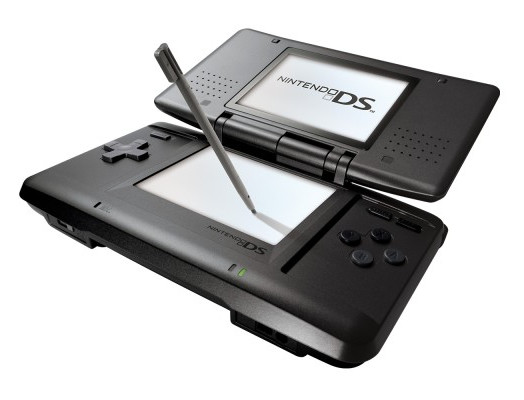
\includegraphics[width=0.4\textwidth]{archivos/nds.jpg}
  \caption{Nintendo DS}
  \textbf{Fuente:} \href{https://www.nintendo.co.uk/Nintendo-DS/Nintendo-DS-Family-Nintendo-UK-s-official-site-Nintendo-DS-Nintendo-DSi-Nintendo-DSi-XL-116380.html}{Nintendo}
  \label{fig:nds1}
\end{figure}

\vspace{0.5cm}

La consola consta de \textbf{ dos pantallas LCD} retroiluminadas con brillo ajustable, siendo una de ellas (la inferior) \textbf{ táctil}, un  \textbf{pad de direcciones},  \textbf{seis botones de acción} (A,B,X,Y, R y L) , \textbf{dos botones de control} (Start y Select) y un \textbf{micrófono}. En su interior posee \textbf{dos procesadores}, un \textbf{ARM946E-S} de 67 MHz que, en general, se encarga de la mayor parte del trabajo ejecutando los \textbf{juegos de NDS} y un \textbf{ARM7TDMI} de 33 MHz, que mueve los juegos de \textbf{GBA} y algunas funciones Wi-Fi. Profundizaremos en ambos procesadores más adelante.

\vspace{0.5cm}

Como curiosidad, las siglas DS significan \textbf{Developer's System} (Sistema de desarrolladores) ya que según la compañía, este sistema ofrece muchas herramientas para que los desarrolladores puedan innovar en sus creaciones. No obstante, también hicieron oficial que estas siglas también hacían referencia a \textbf{Dual Screen}, por su doble pantalla.

\vspace{1cm}

\subsection{Versiones}

Ahora que conocemos un poco más la Nintendo DS original, es importante que analicemos sus posteriores ediciones, ya que nuestro juego debe funcionar en cualquiera de ellas. Debemos conocer qué diferencias significativas existen y tenerlas en cuenta a la hora de desarrollar el juego. Así pues vamos a ir revisando la familia de consolas de Nintendo DS y conociendo sus principales cambios.

\vspace{1cm}

%\subsection{Nintendo DS}

%\begin{figure}[htbp]
%\centering
  %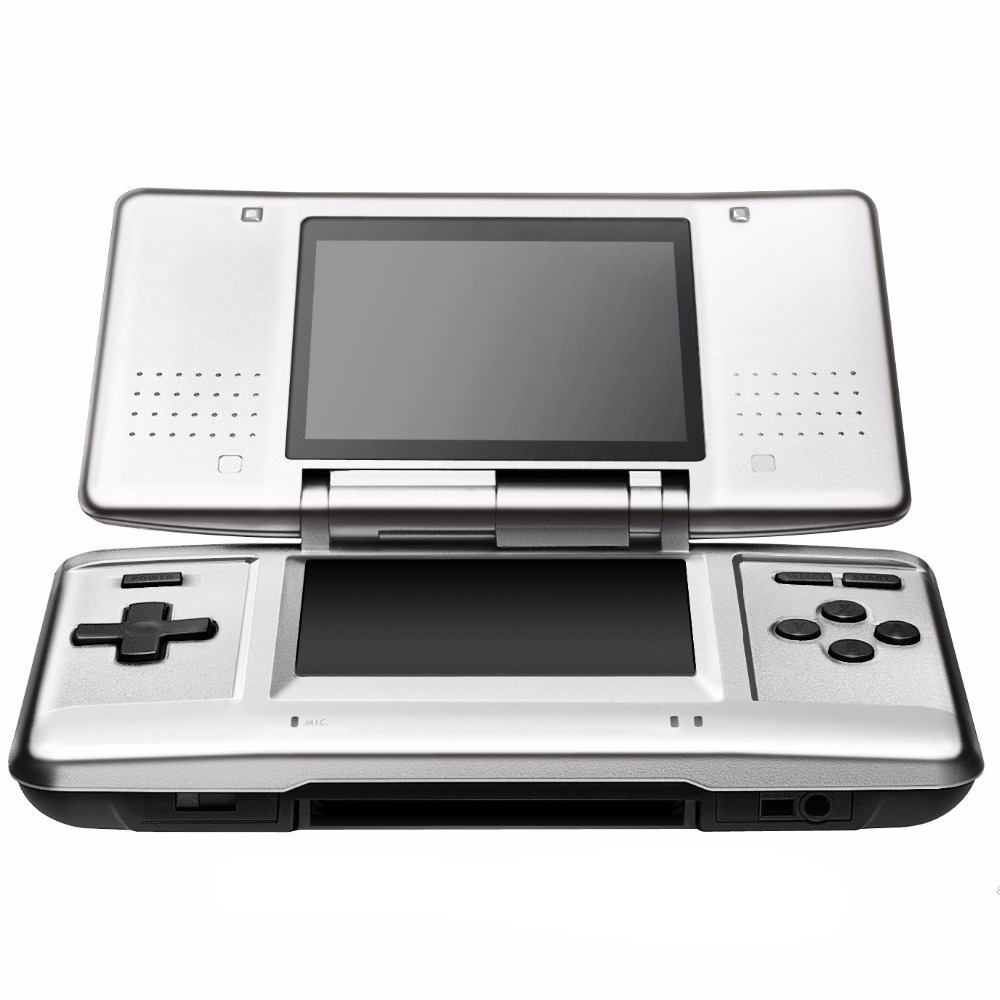
\includegraphics[width=0.3\textwidth]{archivos/nds2.jpg}
 % \caption{Nintendo DS}
  %\label{fig:nds2} %si cambio esto se irá la ref a la *??
%\end{figure}

\subsubsection{Nintendo DS Lite}

Fue creada en \textbf{2006} por Nintendo, es ligeramente \textbf{más pequeña} que su predecesora e incluía una \textbf{carcasa} más elegante. Algunos \textbf{botones} fueron \textbf{relocalizados} y añadía la función de poder elegir entre \textbf{4 niveles de brillo} a diferencia de la original, que solo podía ajustarse al mínimo o al máximo.

\vspace{0.5cm}

\begin{figure}[htbp]
\centering
  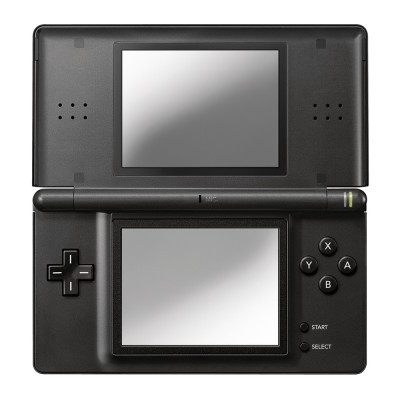
\includegraphics[width=0.3\textwidth]{archivos/ndslite.jpg}
  \caption{Nintendo DS Lite}
    \textbf{Fuente:} \href{https://www.nintendo.co.uk/Nintendo-DS/Nintendo-DS-Family-Nintendo-UK-s-official-site-Nintendo-DS-Nintendo-DSi-Nintendo-DSi-XL-116380.html}{Nintendo}
  \label{fig:ndslite}
\end{figure}

\vspace{1cm}

\subsubsection{Nintendo DSi}

Salió a la venta a finales de \textbf{2008 en Japón} y en \textbf{2009 en el restro del mundo} y se trata de una \textbf{revisión} del modelo de la Nintendo DS Lite. Si bien mantiene muchas características intactas, hay algunas otras que se deben destacar.

\vspace{0.5cm}

\begin{figure}[htbp]
\centering
  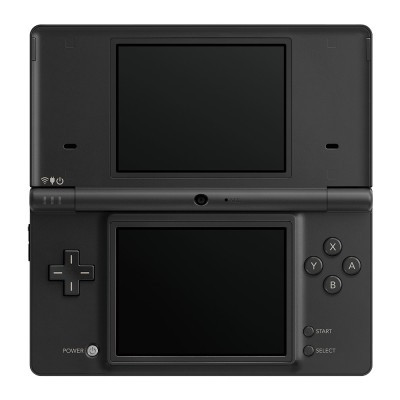
\includegraphics[width=0.3\textwidth]{archivos/ndsi.jpg}
  \caption{Nintendo DSi}
    \textbf{Fuente:} \href{https://www.nintendo.co.uk/Nintendo-DS/Nintendo-DS-Family-Nintendo-UK-s-official-site-Nintendo-DS-Nintendo-DSi-Nintendo-DSi-XL-116380.html}{Nintendo}
  \label{fig:ndsi}
\end{figure}

\vspace{0.5cm}

El primer cambio notable y que a mucha gente no le agradó, fue que \textbf{dejaba de ser compatible} con los juegos de \textbf{GBA}, pues ya no poseía ranura para los cartuchos. Introdujeron una \textbf{cámara delantera} y otra \textbf{trasera}, ambas de 0.3 megapíxeles, con las que podías hacer fotos y editarlas mediante un programa llamado \textbf{Cámara DSi} que venía instalado en la consola por defecto.  Poseía también una ranura para \textbf{tarjetas SD}, en las que podías guardar las fotos de la cámara así como los programas o juegos que descargases de la \textbf{Tienda Nintendo DSi}.

\vspace{0.5cm}

Por último, otras mejoras o diferencias frente a sus modelos originales son una \textbf{mejora de la calidad del audio}, \textbf{aumento} de la \textbf{memoria interna y RAM}, el procesador principal \textbf{ARM9} pasó a ser de 133 MHz (\textbf{aumentando su velocidad}), un \textbf{aumento} ligero del \textbf{tamaño de las pantallas} y \textbf{reducción} de la \textbf{duración de la batería} a 16 horas, siendo de 18 horas y media las originales.

\vspace{0.5cm}

El \textbf{menú principal} de la consola es completamente distinto al de la DS original, pasando a ser bastante \textbf{más personalizable} y con una gran variedad de programas, los cuales algunos de ellos se mantenían desde la DS como el \textbf{Picto-Chat} o la \textbf{Descarga DS}.

\vspace{0.5cm}

\begin{figure}[htbp]
\centering
  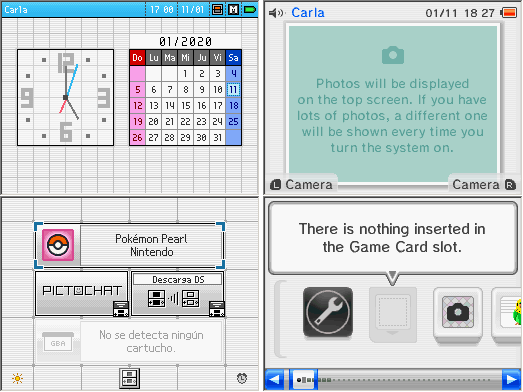
\includegraphics[width=0.6\textwidth]{archivos/nds-ndsi-menu.png}
  \caption{Menú de Nintendo DS (izquierda) frente al de Nintendo DSi (derecha)}
  \label{fig:menu-comparacion} %si cambio esto se irá la ref a la *??
\end{figure}

\vspace{0.5cm}

Fué la primera consola portátil en tener \textbf{bloqueo regional}, no permitiendo que juegos desarrollados en países extranjeros se ejecutasen en la consola si esta era originaria del mismo país.

\vspace{1cm}

\subsubsection{Nintendo DSi XL}

Se trata de un modelo adicional de NDSi que salió a la venta en \textbf{Japón en 2009}, donde originalmente se bautizó como Nintendo DSi LL, llegando a \textbf{España en 2010} donde pasó a llamarse Nintendo DSi XL.

\vspace{0.5cm}

\begin{figure}[htbp]
\centering
  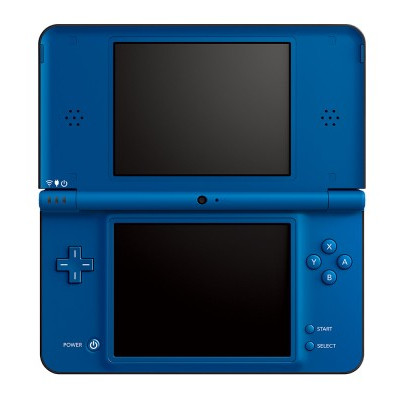
\includegraphics[width=0.3\textwidth]{archivos/ndsixl.jpg}
  \caption{Nintendo DSi XL}
    \textbf{Fuente:} \href{https://www.nintendo.co.uk/Nintendo-DS/Nintendo-DS-Family-Nintendo-UK-s-official-site-Nintendo-DS-Nintendo-DSi-Nintendo-DSi-XL-116380.html}{Nintendo}
  \label{fig:ndsixl} %si cambio esto se irá la ref a la *??
\end{figure}

\vspace{0.5cm}

El principal cambio destacable es el considerable aumento del tamaño de la consola como consecuencia del \textbf{aumento del tamaño de las pantallas} (estas tienen aproximadamente \textbf{una pulgada más} comparadas con la NDSi). En general es una consola perfecta para aquellos que tengan alguna discapacidad visual o les sea difícil o incómodo jugar con las anteriores por su tamaño.

\vspace{1cm}

\subsection{Especificaciones}

En esta sección vamos a conocer los detalles técnicos de la consola y profundizar en los más interesantes para poder entender qué la compone. Podemos ver a continuación una tabla a modo de resumen.
\clearpage

\begin{table}[htbp]

\centering

\begin{tabular}{|l|l|lll}

\cline{1-2}

\textbf{CPU}                & \begin{tabular}[c]{@{}l@{}}ARM946E-S 32bit RISC CPU\\ ARM7TDMI 32bit RISC CPU\end{tabular} &  &  &  \\ \cline{1-2}

\textbf{Velocidad de reloj} & \begin{tabular}[c]{@{}l@{}}(ARM9) 66MHz\\ (ARM7) 33MHz (16MHz en modo GBA)\end{tabular}    &  &  &  \\ \cline{1-2}

\textbf{RAM}                & 4096KB                                                                                     &  &  &  \\ \cline{1-2}

\textbf{VRAM}               & 656KB                                                                                      &  &  &  \\ \cline{1-2}

\textbf{Pantalla}           & 2 pantallas LCD (256x192 px, 3"). Una de ellas táctil.                                                           &  &  &  \\ \cline{1-2}

\textbf{Paleta de colores}  & 18-bit (262144 colores)                                                                    &  &  &  \\ \cline{1-2}

\textbf{Sonido}             & 16 canales de sonido estéreo                                                               &  &  &  \\ \cline{1-2}

\textbf{Comunicación}       & Wifi IEEE 802.11b                                                                          &  &  &  \\ \cline{1-2}

\textbf{Alimentación}       & Batería recargable de ion de litio 850mAh                                                  &  &  &  \\ \cline{1-2}

\textbf{Peso}               & 275g                                                                                       &  &  &  \\ \cline{1-2}

\textbf{Dimensiones}        & 148.7mm × 84.7mm × 28.9mm                                                                  &  &  &  \\ \cline{1-2}

\end{tabular}
\caption{Especificaciones técnicas de la NDS}
\end{table}

Para profundizar más acerca de los procesadores de la consola, su memoria de vídeo, zonas hardware específicas para gráficos, sonido y ROM, visita el \hyperref[anexo]{\textbf{Anexo I}}.

\vspace{1cm}


\section{Estudio de mercado}

Si bien la NDS fue una consola revolucionaria por su gran número de ventas así como el éxito de sus grandes títulos, hoy en día ya no se producen juegos para ésta, pues ha sido \textbf{sucedida por la 3DS}. Es por esto que el mercado a día de hoy se reduce a fanáticos que desean comprar en buen estado estos juegos y lo hacen mediante la venta de \textbf{segunda mano}.

\vspace{0.5cm}

No obstante, existe la llamada \textbf{\textit{Scene}}, conformada por los programadores e informáticos que desarrollan \textbf{aplicaciones y juegos no oficiales} para sistemas como es la NDS entre muchas otras. La existencia de este tipo de comunidades son muy buenas ya que gracias a foros o \textit{hashtags} como el de \#dsdev en Twitter puedes llegar a más público, haciendo que quizás se interesen por tu proyecto.

\vspace{1cm}

\section{Algoritmo de reconocimiento de escritura}

%LINKS: COMENTADOS

%http://cravesoft.free.fr/PAlibDocEng/html/group___reco.html#ga925cec3c4c9e826e8c07ee5a2366feb

%https://github.com/jichu4n/palm-os-sdk

%https://riunet.upv.es/bitstream/handle/10251/11576/memoria.pdf?sequence=1

%https://devkitpro.org/wiki/PAlib

%https://azydream.tistory.com/55

%https://github.com/atgreen/RTEMS/blob/master/c/src/lib/libbsp/arm/nds/touchscreen/reco.c

%https://es.wikipedia.org/wiki/Graffiti_(Palm_OS)

%http://patft.uspto.gov/netacgi/nph-Parser?Sect1=PTO1&Sect2=HITOFF&d=PALL&p=1&u=%2Fnetahtml%2FPTO%2Fsrchnum.htm&r=1&f=G&l=50&s1=5596656.PN.&OS=PN/5596656&RS=PN/5596656                  o                 https://patents.google.com/patent/US5596656

Algo esencial que necesitaremos para llevar a cabo este proyecto es un \textbf{algoritmo} que nos permita \textbf{reconocer el patrón que dibuje el usuario} en la pantalla táctil de entre unos que nosotros tengamos definidos. 

\vspace{0.5cm}

El desarrollo de un \textit{software} de estas características es sin duda algo que puede hacer que algunos desarrolladores se lleven las manos a la cabeza. Si bien es cierto que a día de hoy existen gran número de programas de pago o incluso integrados en nuestros teléfonos y ordenadores que son capaces de distinguir caracteres dibujados por usuarios, hay muy pocos de ellos de código abierto. Por suerte, tenemos un ejemplo de un \textit{software} así en el contexto que nos interesa.

\vspace{0.5cm}

Para el desarrollo en NDS existía una librería llamada \textbf{PAlib} que surgió en los primeros años de desarrollo \textit{homebrew} cuyo objetivo, al igual que \textbf{libnds}, era facilitar las tareas al programador. No obstante, a pesar de haber sido bien acogida por los usuarios por su sencillez y fácil uso, los encargados de mantener el conjunto de librerías y herramientas de \textbf{devkitPro} afirmaban que esta librería estaba \textbf{mal diseñada y provocaba serios fallos} en la consola tales como corrupciones de la tarjeta SD. Es por ello que devkitPro, del cual hablaremos más adelante, dejó de dar soporte a esta librería\footnote{https://devkitpro.org/wiki/PAlib} y ésta tras un tiempo esta cerró su página web y dejó de actualizarse. A día de hoy, parte de su documentación y código fuente siguen publicados en internet gracias a usuarios que lograron recuperarlas del archivo.

\vspace{0.5cm}

Lo que nos interesa a nosotros de esta librería es precisamente que implementó un \textbf{algoritmo de reconocimiento de escritura manuscrita} similar a otro más conocido como es \textbf{Graffiti de Palm}, pues en ambos la forma de dibujar los caracteres es la misma. Así pues, vamos a comprender a continuación cómo solucionan el problema ambos algoritmos.

\vspace{0.5cm}

\subsubsection{Graffiti de PAlib}

Como hemos comentado, este algoritmo de PAlib nos da como resultado el carácter al que más se parezca el dibujado por el usuario. Los trazos y sus respectivos carácteres son los mostrados en la siguiente figura, donde como podemos ver, no hay números ni algunos caracteres especiales como la 'ñ'. No obstante, esto es compensado con la posibilidad de poder incorporar \textbf{nuestros propios trazos}. 

\vspace{0.5cm}

\begin{figure}[htbp]
\centering
  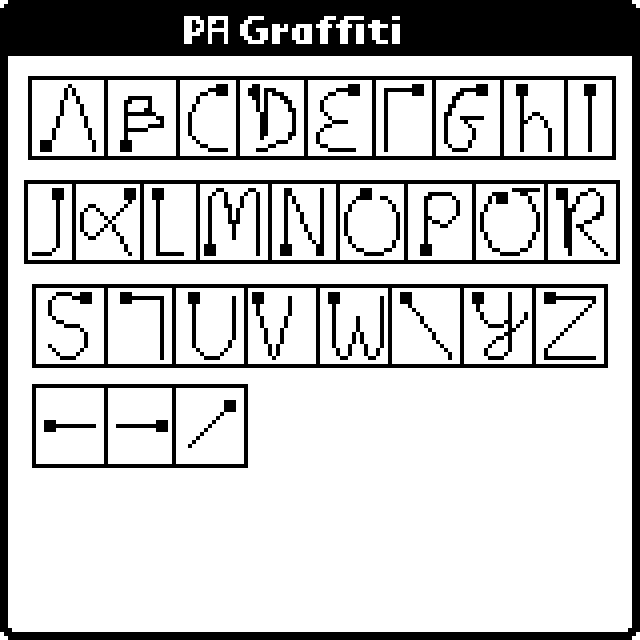
\includegraphics[width=0.3\textwidth]{archivos/pagraffiti.png}
  \caption{Caracteres y su trazo correspondiente de PA Graffiti}
  \textbf{Fuente:} \href{https://web.archive.org/web/20070708175646/http://www.palib.info/Reco/PAGraffiti.gif}{Documentación de PAlib (Recuperada del archivo)}
  \label{fig:pagraffiti}
\end{figure}

\vspace{0.5cm}

El algoritmo funciona de la siguiente manera: 

\vspace{0.5cm}

\begin{itemize}
 \item Guarda en un array cada par de coordenadas (x1,y1), ... , (xn,yn) que conforman el \textbf{trazo} introducido por el usuario.
 
 \item De toda esa lista de puntos, escoge \textbf{17} muestras para computarlas. 
 
 \item Calcula el \textbf{ángulo entre cada par de puntos} y le \textbf{asigna un carácter} dependiendo del rango en el que caiga dicho ángulo.
 
 \item \textbf{Compila todos los caracteres} de los ángulos calculados y genera una cadena de 16 caracteres que define dicho trazo.
 
 \item Busca dentro de unos trazos que ya tiene definidos, aquella \textbf{cadena de caracteres} que sea \textbf{más parecida} a la introducida por el usuario.
\end{itemize}

\vspace{0.5cm}

Como observamos, lo que básicamente hace el algoritmo es \textbf{caracterizar la línea con una cadena de caracteres} sirviendose del ángulo que forman los puntos de esta misma. Una vez calcula el ángulo que forman dos puntos, para saber qué caracter asignarle se vale de una circunferencia la cual está dividida en \textbf{32 rangos} como se ven en la siguiente figura.

\vspace{0.5cm}

\begin{figure}[htbp]
\centering
  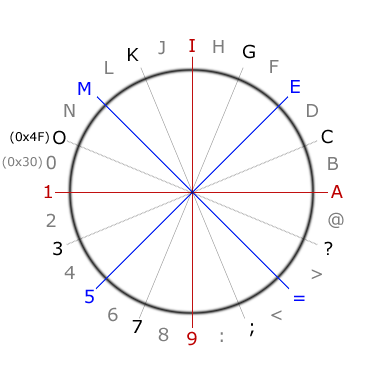
\includegraphics[width=0.5\textwidth]{archivos/recocircle.png}
  \caption{Correspondencia entre caracteres y los 32 rangos de ángulos.}
  \textbf{Fuente:} \href{https://azydream.tistory.com/55}{azyDream}
  \label{fig:recocircle}
\end{figure}

\vspace{0.5cm}

Así pues, un carácter como por ejemplo la letra 'i' equivaldría a la cadena '9999999999999999', pues al dibujarse completamente en vertical desde arriba hacia abajo todos los ángulos calculados caerían en el rango que equivale al 9.

\vspace{0.5cm}

En la figura siguiente veríamos un ejemplo de cuál sería la cadena asignada al trazo mostrado en blanco. Las líneas azules representan los 17 puntos de muestra. Como se ve, los primeros caracteres del trazo son A, pues el ángulo entre puntos es de 0 grados y conforme el trazo va descendiendo se le van asignando las letras de los rangos consecuentes.

\vspace{0.5cm}

\begin{figure}[htbp]
\centering
  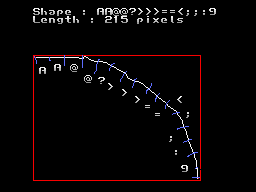
\includegraphics[width=0.5\textwidth]{archivos/recoex.png}
  \caption{Ejemplo de asignación de una cadena de caracteres a un trazo.}
  \textbf{Fuente:} \href{https://azydream.tistory.com/55}{azyDream}
  \label{fig:recoex}
\end{figure}


\vspace{0.5cm}

Esta forma de trabajar del algoritmo es lo que permite que puedas \textbf{introducir tus propios diseños de forma sencilla para el programador}, pues solo tienes que dibujar el patrón que deseas en un proyecto a parte y haciendo llamadas a las funciones de crear una forma te devolverían una cadena que identifica dicho trazo. De hecho, el algoritmo te da la posibilidad de analizar formas en base a unas que tiene predefinidas o las tuyas propias.

\vspace{0.5cm}

\subsubsection{Graffiti de Palm}

\textbf{Graffiti} es un \textit{software} de reconocimiento de escritura manuscrita desarrollado por el ingeniero informático \textbf{Jeff Hawkins} en \textbf{Palm} para las \textbf{PDAs} con sistema operativo PalmOS. Dicho \textit{software} crea una ligera modificación y simplificación de los carácteres alfabéticos, como podemos ver en la siguiente figura, para que puedan ser dibujados con un lápiz táctil sobre una pantalla y sin levantarlo hasta completar el trazo.

\clearpage


\begin{figure}[htbp]
\centering
  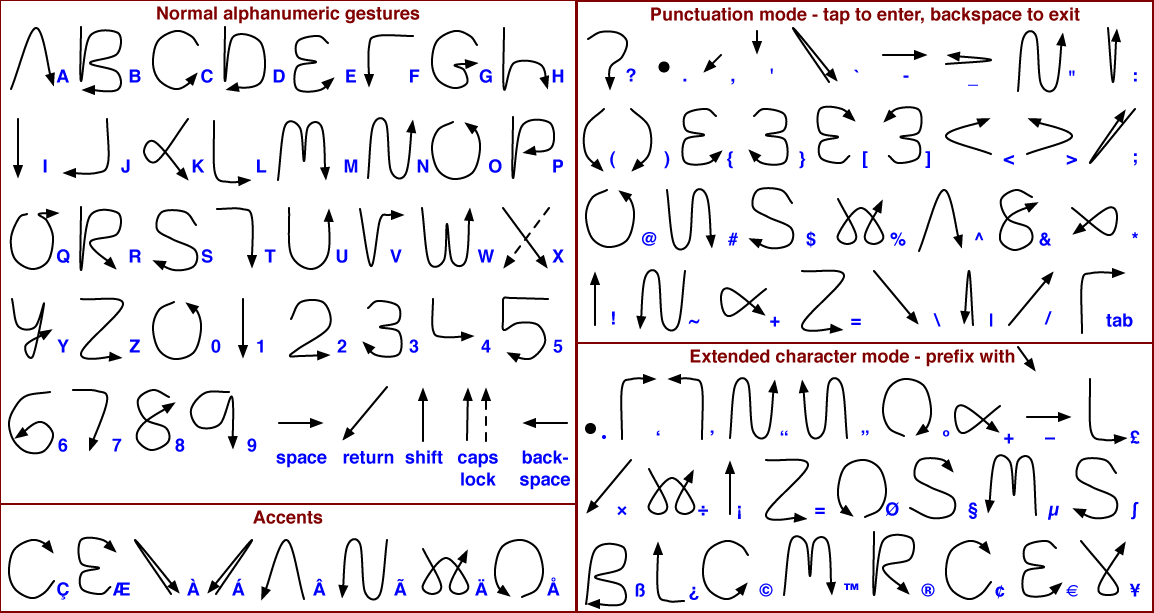
\includegraphics[width=0.6\textwidth]{archivos/palm_gestures.png}
  \caption{Gestos usados en PalmOS para definir los distintos caracteres}
\textbf{Fuente:} \href{https://es.wikipedia.org/wiki/Graffiti_(Palm_OS)#/media/Archivo:Palm_Graffiti_gestures.png}{IMewbot}
  \label{fig:palm_gestures}
\end{figure}

\vspace{0.5cm}

No obstante, Graffiti tuvo que ser \textbf{retirado y más tarde sustituido} por una nueva versión de este ya que la compañía \textbf{Xerox demandó a Palm} porque su \textit{software} de reconocimiento de escritura violaba la patente de Xerox sobre \textbf{tecnología Unistrokes}. Esto fue así porque Palm consiguió una demo de dicha tecnología antes de desarrollar su propio sistema.

\vspace{0.5cm}

Esto es importante comentarlo, pues a continuación explicaremos cómo funciona el algoritmo de la tecnología Unistrokes tal y como está reflejado en la pantente USPTO nº 5596656\footnote{https://patents.google.com/patent/US5596656}, pero debemos  tener en cuenta que la primera versión de Graffiti funciona de la misma manera.

\vspace{0.5cm}

Así pues, vamos a describir brevemente lo que hace el algoritmo para identificar el trazo:

\vspace{0.5cm}

\begin{itemize}
 \item Guardar en una lista ordenada cada par de coordenadas (x1,y1), . . . , (xn,yn) que conforman el \textbf{trazo}.
 \item \textbf{Filtrar dicha lista} para eliminar el posible ruido y suavizar así el trazo para facilitar el cálculo.
 \item Comprobar si se trata de una \textbf{línea recta} y, si es así, calcular la pendiente de esta. Usar esa pendiente para comprobar los caracteres que se generan con una línea, como por ejemplo i, 1, espaciado... Y terminar la búsqueda.
 \item Si no se trata de una línea recta, \textbf{normalizar} el trazo para que quepa en una caja cuadrada y calcular las siguientes características:
 
 \end{itemize}
 
 El \textbf{desplazamiento en el eje x} entre el origen y el final
  \begin{equation}
dx=xn-x1
\end{equation}

 El \textbf{desplazamiento en el eje y} entre el origen y el final
  \begin{equation}
dy=yn-y1
\end{equation}

El \textbf{desplazamiento entre el origen y el punto medio del trazo en el eje x}
\begin{equation}
 dx_{x1-xn/2}=x(n/2)-x1
\end{equation}

El \textbf{desplazamiento entre el origen y el punto medio del trazo en el eje y}
\begin{equation}
dy _{y1-yn/2}=y(n/2)-y1
\end{equation}

La \textbf{suma de las longitudes} de las líneas que unen cada punto con su predecesor \textbf{proyectado en el eje x}
\begin{equation}
lengthxtot = length_x(x1,x2) + length_x(x2,x3) + ... + length_x(xn-1,xn)
\end{equation}

La \textbf{suma de las longitudes} de las líneas que unen cada punto con su predecesor \textbf{proyectado en el eje y}
\begin{equation}
lengthytot = length_y(y1,y2) + length_y(y2,y3) + ... + length_y(yn-1,yn)
\end{equation}


\begin{itemize}
 \item Calculadas estas características, elegir el carácter que más se parece de una \textbf{tabla} como la siguiente:
\end{itemize}

\begin{table}[hbtp]
\centering
\begin{tabular}{c|c|c|c|c|c|c|}
\cline{2-7}
\multicolumn{1}{l|}{}           & dx        & dy        & dx(x1-xn/2) & dy(y1-yn/2) & length x tot & length y tot \\ \hline
\multicolumn{1}{|c|}{a}         & 0.0       & -1.0      & 0.0         & -0.5        & 0.0          & 1.0          \\ \hline
\multicolumn{1}{|c|}{b}         & 0.0       & 1.0       & 1.0         & 0.5         & 2.0          & 1.0          \\ \hline
\multicolumn{1}{|c|}{c}         & 0.0       & -1.0      & -1.0        & -0.5        & 2.0          & 1.0          \\ \hline
\multicolumn{1}{|c|}{d}         & 0.0       & 1.0       & -1.0        & 0.5         & 2.0          & 1.0          \\ \hline
\multicolumn{1}{|c|}{e}         & -1.0      & 0.0       & -0.5        & 0.0         & 1.0          & 0.0          \\ \hline
\multicolumn{1}{|c|}{{[}...{]}} & {[}...{]} & {[}...{]} & {[}...{]}   & {[}...{]}   & {[}...{]}    & {[}...{]}    \\ \hline
\end{tabular}
\caption{Datos de cada letra estudiados.}
\label{table:tablepalm}
\end{table}

\begin{itemize}
 \item Si el resultado es una U o una O, determinar si el trazo gira en el \textbf{sentido horario o antihorario} para afirmar si es una U o una O respectivamente.
\end{itemize}

\vspace{0.5cm}

Como podemos ver, el algoritmo calcula una serie de \textbf{valores que caracterizan la línea} y los compara con los que han estimado para los distintos caracteres que pueden dibujar. No obstante, debemos detenernos a entender dos de ellos pues son los que más confusión pueden provocar: lengthxtot y lengthytot.

\vspace{0.5cm}

Tal y como se explicaba anteriormente, este valor representa para cada eje, la suma de las longitudes de unas línea simaginarias desde un punto hasta su predecesor. Es importante no confundir este concepto con la distancia del punto inicial al final, pues si bien pueden coincidir en algunos casos, no significan lo mismo. Por ejemplo, imaginemos un trazo conformado por 3 puntos completamente colocados en vertical y separados en una unidad. En este caso, ambos valores serían iguales, 3, pero si el trazo lo modificamos para que tenga un cuarto punto inferior al tercero, ahora la longitud sería mayor a 3 y la distancia menor a tres, pues habríamos añadido un segmento más en el caso de la longitud y por el contrario, la distancia entre el punto inicial y final ahora es menor.

\vspace{0.5cm}

La siguiente figura muestra un ejemplo gráfico de cómo se representa estos valores:

\vspace{0.5cm}

\begin{figure}[htbp]
\centering
  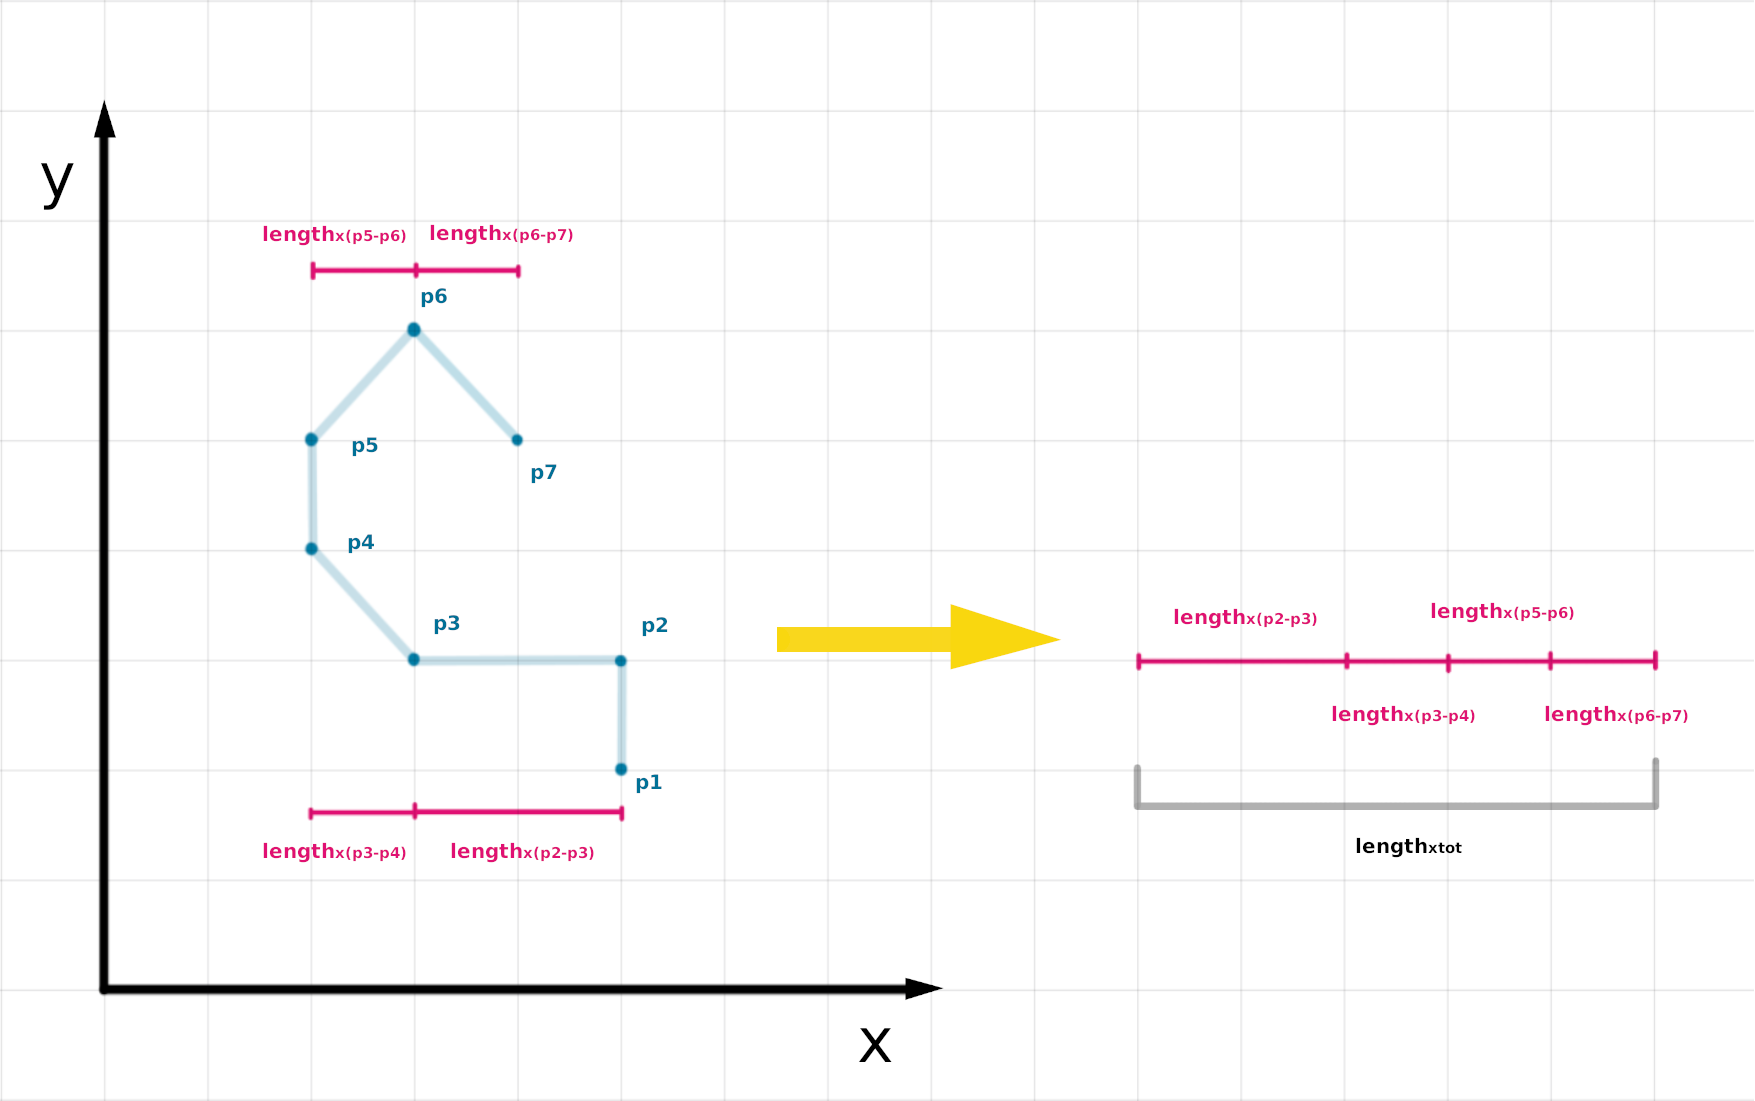
\includegraphics[width=0.8\textwidth]{archivos/vertline_x.png}
  \caption{Ejemplo gráfico del cálculo de la longitud total en el eje x}
  \label{fig:vertline_x}
\end{figure}

\clearpage

\begin{figure}[htbp]
\centering
  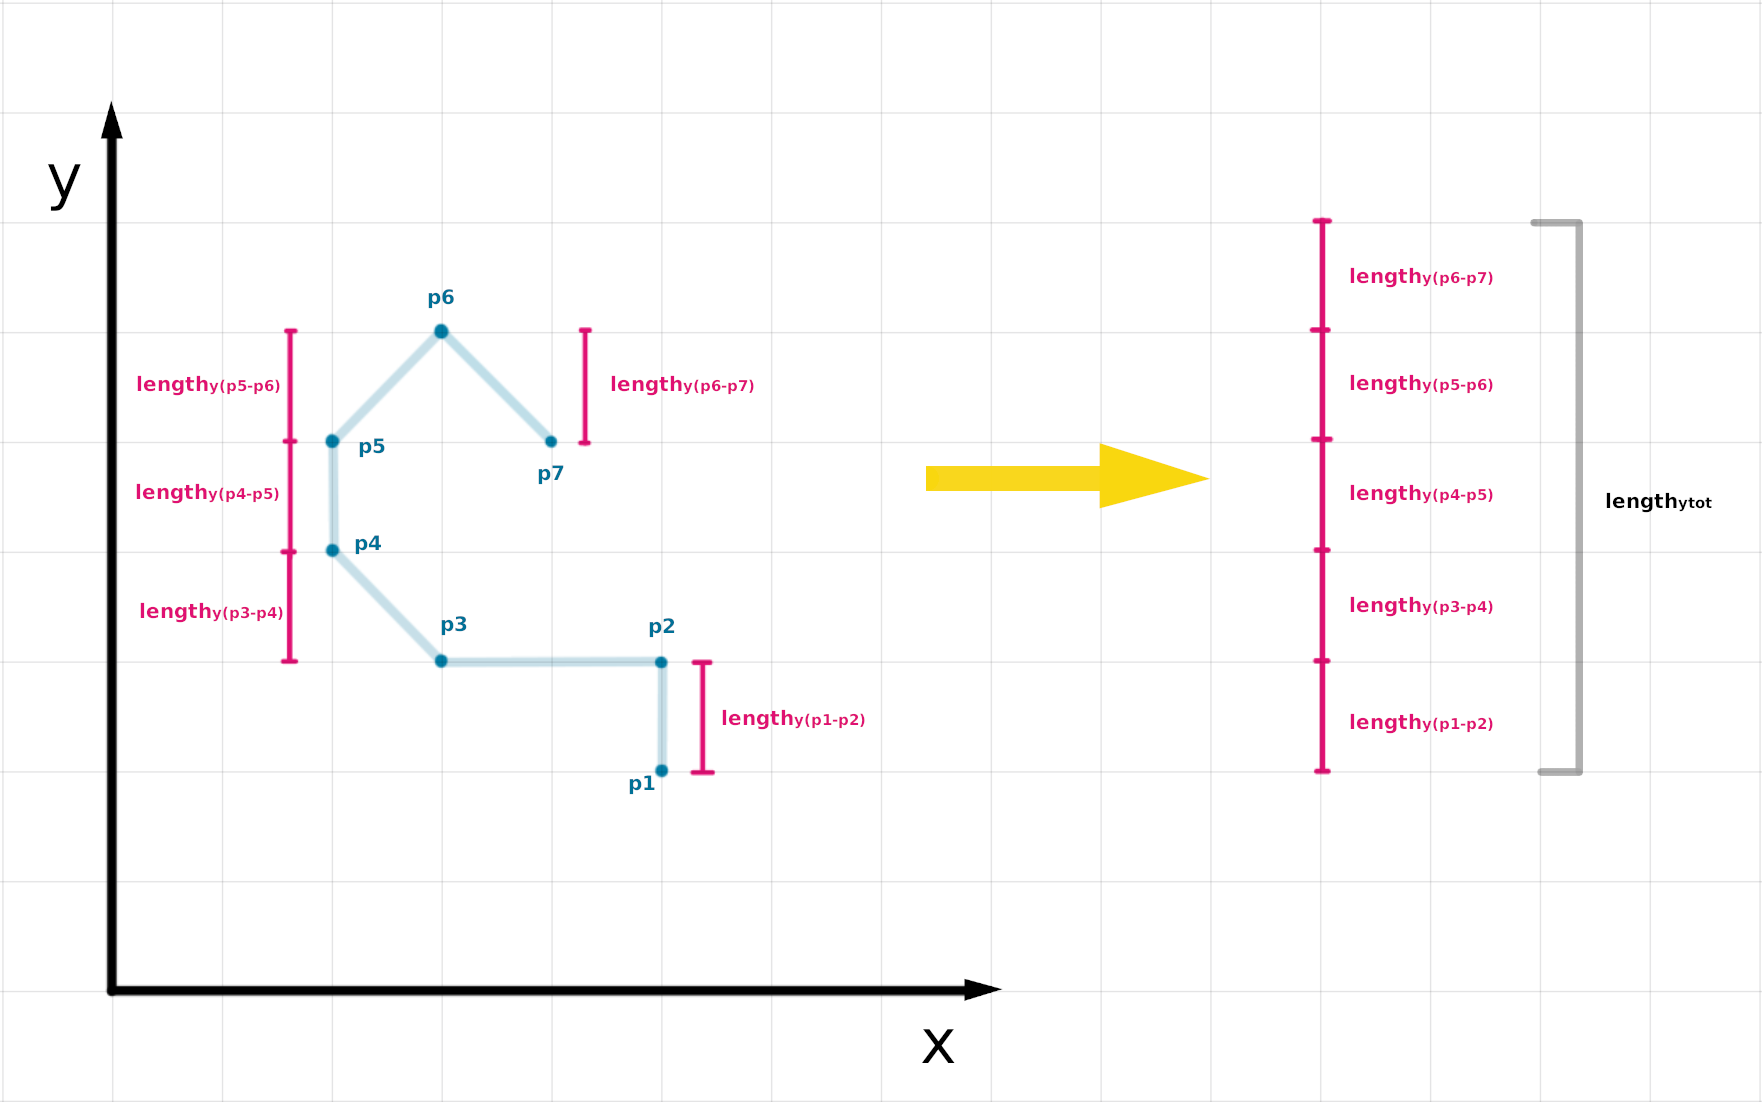
\includegraphics[width=0.8\textwidth]{archivos/vertline_y.png}
  \caption{Ejemplo gráfico del cálculo de la longitud total en el eje y}
  \label{fig:vertline_y}
\end{figure}

\vspace{0.5cm}

Una vez comprendemos estos algoritmos un poco más en detalle podemos valorar si implementarlos o crear el nuestro propio. Si bien implementarlos otorgaría más facilidades y sería más eficaz y rápido a la hora de funcionar, se ha decidido crear uno propio, con el fin de \textbf{aprender} un poco más sobre las bases \textbf{matemáticas} que hacen que todos estos algoritmos puedan funcionar. En un entorno más laboral es muy importante que no nos dediquemos a reinventar la rueda, sin enmbargo este entorno sigue siendo académico, con lo cual es más enriquecedor aprender un poco más sobre estos aspectos. No obstante, es muy importante analizar estas soluciones y tenerlas presentes ya que en el caso de no poder llegar a crear un algoritmo propio, estos podrían servir de colchón.

\vspace{0.1cm}


\section{Referentes}

En esta sección analizaremos los \textbf{juegos en los que nos hemos basado} para elaborar un diseño de nuestro juego, ya sea en las mecánicas, arte, pantallas, o incluso las formas en la que los desarrolladores implementaron las funcionalidades.

\vspace{0.5cm}

\subsection{Magic Cat Academy }

Se trata de un juego para \textbf{navegador} que fue creado como \textbf{Doodle} de Google para celebrar \textbf{Halloween} del año 2016.

\clearpage


\begin{figure}[htbp]
\centering
  
\includegraphics[width=0.6\textwidth]{archivos/doodle.png}
  \caption{Doodle Halloween 2016}
  \label{fig:doodle}
\end{figure}

\vspace{0.5cm}

En este juego seremos Momo, una gata cuyo \textbf{objetivo es recuperar el libro de hechizos mágicos} de su escuela que los espíritus han robado. Para ello, debemos enfrentarnos a ellos  \textbf{dibujando en la pantalla} con ayuda del ratón los  \textbf{símbolos} que llevan justo en la parte superior para derrotarlos, avanzar por las salas de la escuela y dar con el jefe. Si algún fantasma nos  \textbf{alcanza} perderemos una {vida} de un  \textbf{total de 5} y al quedarnos sin ellas acabará la partida. Además, cuanto más rápido y mejor realicemos los patrones de los enemigos conseguiremos acumular  \textbf{combos} que nos aumentarán la  \textbf{puntuación}.

\begin{figure}[htbp]
\centering
  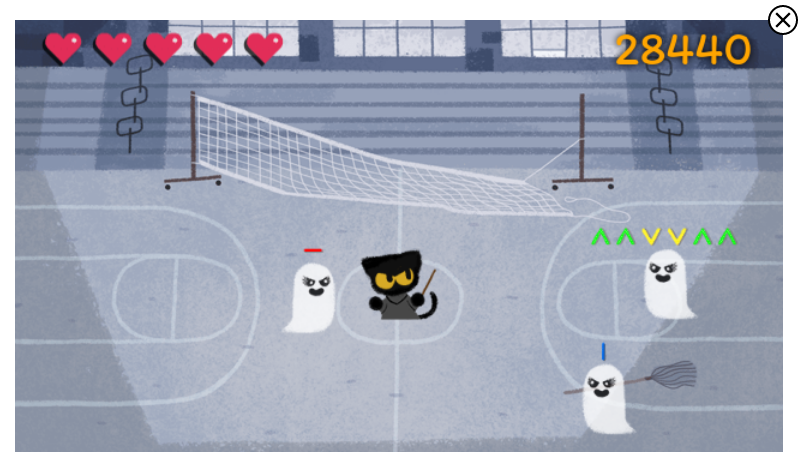
\includegraphics[width=0.6\textwidth]{archivos/juego.png}
  \caption{Cuarto nivel del juego, el gimnasio}
  \label{fig:halloweencat1}
\end{figure}

\vspace{0.5cm}

El juego consta de \textbf{5 niveles} más un nivel de \textbf{jefe final}. En cada nivel hemos de derrotar a una serie de fantasmas y a un jefe con un comportamiento \textbf{único y característico}. A medida que los niveles van avanzando la \textbf{dificultad aumenta}, pues la \textbf{velocidad} de los fantasmas es mayor y también empiezan a aparecer enemigos con \textbf{combinaciones de patrones más complejas y largas}.

\vspace{0.5cm}

Los tipos de patrones que nos podemos encontrar son:

\begin{itemize}
  \item \textbf{Línea vertical:} Por sí solo no tiene efecto diferente, puede combinarse con los demás.
  \item \textbf{Línea horizontal:} Por sí solo no tiene efecto diferente, puede combinarse con los demás.
  \item \textbf{Flecha hacia arriba ($\wedge$):} Por sí solo no tiene efecto diferente, puede combinarse con los demás.
  \item \textbf{Flecha hacia abajo ($\vee$):} Por sí solo no tiene efecto diferente, puede combinarse con los demás.
  \item \textbf{Rayo:} Este patrón es más fuerte que los anteriores, si lo dibujamos cuando hay varios enemigos en pantalla afectará a todos, quitándole un par de símbolos a cada enemigo. Puede combinarse con los demás
  \item \textbf{Corazón:} Aparece de vez en cuando siempre que no tengamos la vida a tope, si lo dibujamos conseguiremos recuperar una unidad de vida.
\end{itemize}

\vspace{0.5cm}

El \textbf{nivel del jefe final} es algo distinto a los demás ya que no sigue la estructura que estos mantenían. En este nivel deberemos derrotar primero a una serie de fantasmas y después dibujar una combinación de patrones muy larga que el jefe posee para hacerle daño antes de que nos alcance. Esto se deberá \textbf{repetir tres veces}, y por supuesto la velocidad y complejidad aumenta cuanto más cerca estemos de derrotarlo.

\begin{figure}[htbp]
\centering
  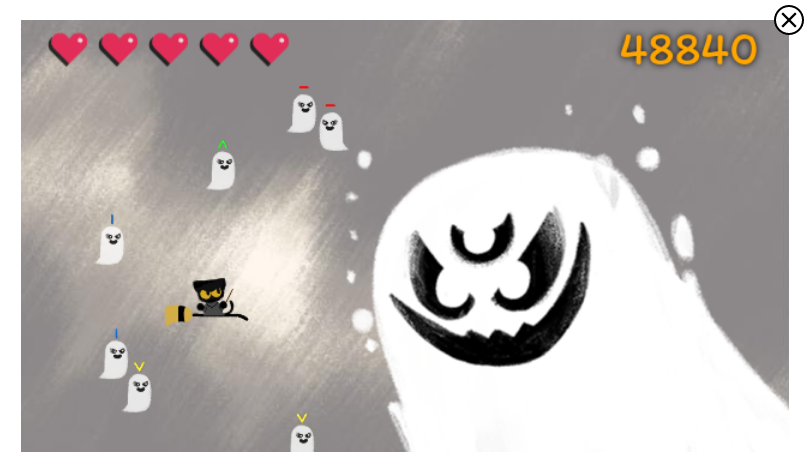
\includegraphics[width=0.6\textwidth]{archivos/jefe-horda.png}
  \caption{Primera fase del jefe donde aparecen enemigos.}
  \label{fig:jefe1}
\end{figure}

\clearpage

\begin{figure}[htbp]
\centering
  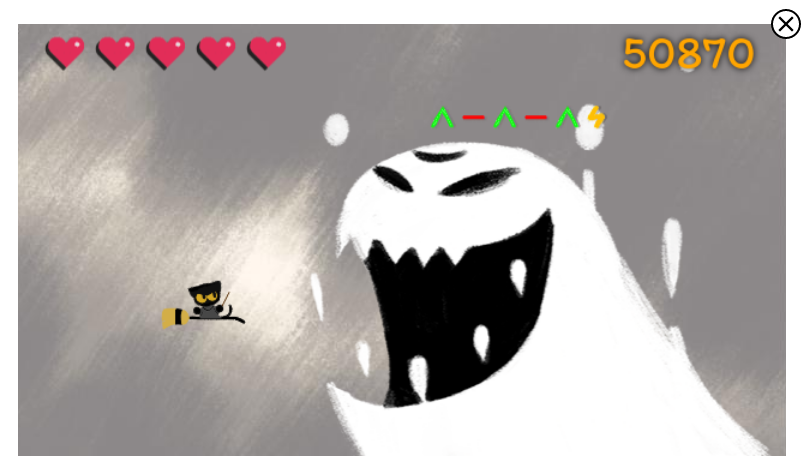
\includegraphics[width=0.6\textwidth]{archivos/jefe-ataque.png}
  \caption{Segunda fase del jefe donde le atacamos diréctamente}
  \label{fig:jefe2}
\end{figure}

\vspace{0.5cm}

Como ya se ha comentado, el jugador puede ir acumulando combos para mejorar su puntuación. Tanto si ganamos la partida como si la perdemos, podremos \textbf{compartir en las redes sociales nuestra puntuación}. Esto es una buena idea ya que permite que los usuarios compartan sus experiencias con otros y les inciten a jugar ya que aporta cierto factor de \textbf{competitividad}.

\begin{figure}[htbp]
\centering
  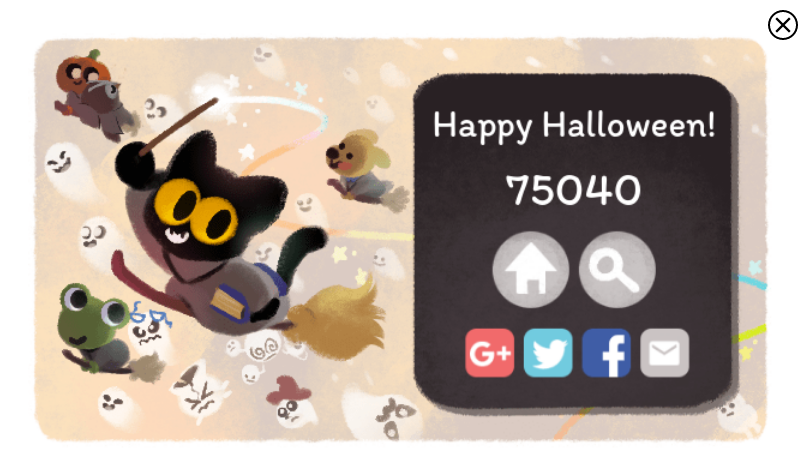
\includegraphics[width=0.6\textwidth]{archivos/pantalla-win.png}
  \caption{Pantalla que aparece al completar el juego}
  \label{fig:halloweenwin}
\end{figure}

\clearpage

\begin{figure}[htbp]
\centering
  
\includegraphics[width=0.6\textwidth]{archivos/pantalla-game-over.png}
  \caption{Pantalla que aparece al perder todas tus vidas.}
  \label{fig:halloweengo}
\end{figure}

Como curiosidad, el juego fue desarrollado por 4 grupos de aproximadamente 4 o 5 personas cada uno. Constaban de un grupo de arte, otro de producción, uno de ingenieros y uno de ``ayuda extra'' donde se realizaba la música.

\vspace{0.5cm}

Ahora bien, hemos elegido este juego como \textbf{principal referente} en cuanto a las \textbf{mecánicas}. Diseñaremos el juego de modo que la esencia y jugabilidad sean prácticamente las mismas. Creemos que un juego de estas características es algo sencillo pero que puede ser muy\textbf{ escalable}, facilitando el desarrollo por iteraciones. También es\textbf{ divertido} y un candidato perfecto para la NDS ya que parece estar hecho para jugarlo con una \textbf{pantalla táctil}.

\vspace{1cm}

\subsection{Una pausa con... Brain Training Ciencias}

Una pausa con... Brain Training o también conocido como Brain Age Express en América, se trata de una serie \textbf{tres juegos educacionales de resolver puzzles} desarrollados por Nintendo y publicados en el servicio \textbf{DSi Ware} de manera \textbf{gratuita} en 2009 en Europa.

\vspace{0.5cm}

Estos tres juegos se tratan de un \textbf{recopilatorio} de los puzzles que más les habían gustado a los jugadores de los \textbf{títulos previos} como Brain Training ¿Cuántos años tiene tu cerebro? y su secuela Más Brain Training para NDS. No obstante, le daban una vuelta de tuerca a estos puzzles haciéndolos \textbf{más desafiantes y divertidos}, incluso integraban el uso de la \textbf{cámara} al ser un proyecto para DSi.

\clearpage

\begin{figure}[htbp]
\centering
  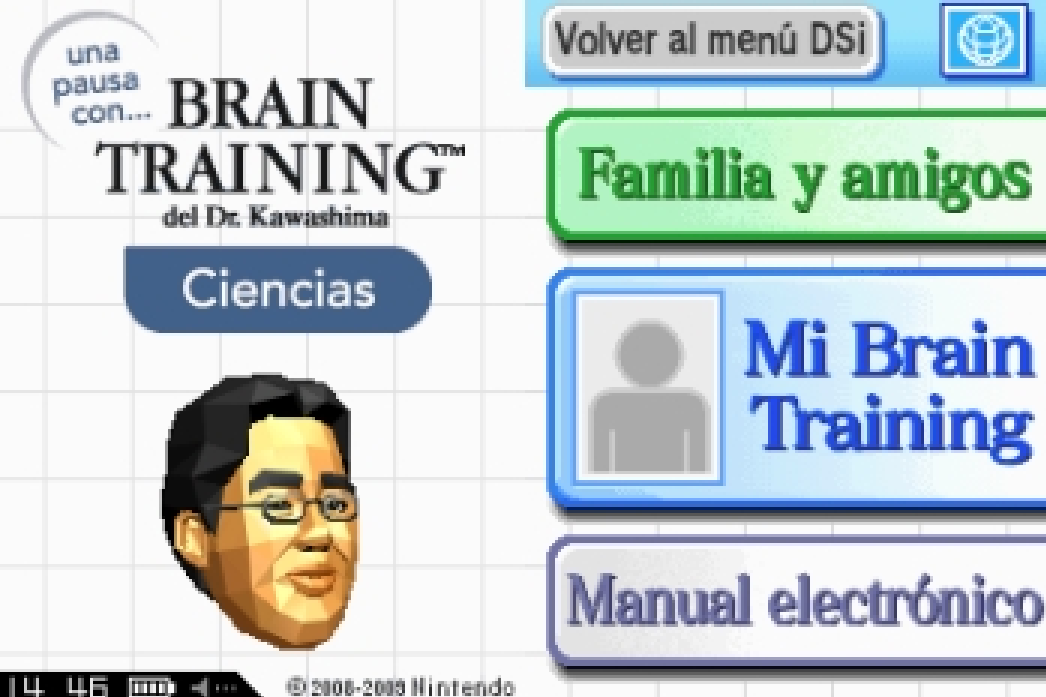
\includegraphics[width=0.6\textwidth]{archivos/brain.png}
  \caption{Menú principal de Una pausa con... Brain Training Ciencias}
  \textbf{Fuente:} \href{https://www.nintendo.es/Juegos/Nintendo-DSiWare/Una-pausa-con-Brain-Training-Ciencias-261960.html}{Nintendo}
  \label{fig:sbraintraining1}
\end{figure}

\vspace{0.5cm}

Todos los títulos de esta saga tienen un mismo \textbf{objetivo}: jugar unos minutos \textbf{diariamente} a una serie de puzzles de \textbf{cálculo}, \textbf{memorización de imágenes o datos} e incluso ejercicios de \textbf{ortografía y lectura}, con el fin de \textbf{ejercitar el cerebro}. No obstante, también proporciona la opción de jugar a dichos puzzles de manera individual e incluso tienen un \textbf{modo sudoku}.

\vspace{0.5cm}

Volviendo a nuestro referente, como hemos comentado se trata de una serie de tres juegos divididos en \textbf{categorías} de \textbf{ciencias, letras y sudoku}. Por una razón que no se hizo oficial, Nintendo quitó del servicio de DSi Ware la edición de sudokus, mientras que las otras dos se mantuvieron e incluso venían preinstaladas en las NDSi americanas. En concreto nos vamos a centrar en la edición de ciencia, pues hay un puzzle particular que tiene bastante relación con nuestro juego: el \textbf{Suma y Sigue}.

\begin{figure}[htbp]
\centering
  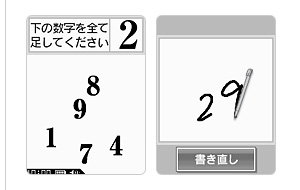
\includegraphics[width=0.6\textwidth]{archivos/brain-sumtotaled1.jpg}
  \caption{Minijuego Suma y Sigue en su modo normal}
    \textbf{Fuente:} \href{https://www.nintendo.co.jp/ds/dsiware/kndjknrj/training2/index.html}{Nintendo}
  \label{fig:sumtotaled1}
\end{figure}

\vspace{0.5cm}

En este minijuego debemos realizar la \textbf{suma} de los \textbf{números} que veremos esparcidos por la pantalla y escribir el resultado en la pantalla táctil \textbf{lo antes posible}. Posee \textbf{dos modos de juego}, uno normal que es el que acabamos de explicar y otro \textbf{arcade}, el que nos interesa. El objetivo del modo arcade es exactamente el mismo, realizar la suma de números, pero con el añadido de que los números ahora no están colocados aleatoriamente en la pantalla, si no forman el cuerpo de un \textbf{enemigo} que se va acercando hacia el jugador para quitarle vida. Este modo otorga un factor más \textbf{desafiante} al juego ya que en el primer modo si fallamos la operación obtendremos peor resultado en la prueba, mientras que en el modo arcade al tener un máximo de tres vidas y ver cómo los enemigos se acercan provoca \textbf{presión} en el jugador.

\begin{figure}[htbp]
\centering
  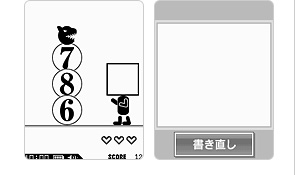
\includegraphics[width=0.6\textwidth]{archivos/brain-sumtotaled2.jpg}
  \caption{Minijuego Suma y Sigue en su modo arcade}
  \textbf{Fuente:} \href{https://www.nintendo.co.jp/ds/dsiware/kndjknrj/training2/index.html}{Nintendo}
  \label{fig:sumtotaled2}
\end{figure}

La razón por la que se ha elegido este minijuego como referente es por poseer algunas \textbf{características adicionales} que Magic Cat Academy no posee con respecto a los enemigos y que podrían aportar más diversión si se \textbf{mezclan}. Por ejemplo, los enemigos a veces se esconden haciendo que \textbf{no se puedan ver} parte de sus números, también dichos números \textbf{se mueven} alrededor del cuerpo de dicho enemigo, haciendo que sea más complicado realizar el cáclulo.

\vspace{1cm}

\subsection{Lost Magic}

Lost Magic es un juego \textbf{RPG} de \textbf{estrategia en tiempo real} desarrollado por \textbf{Taito} para NDS y publicado en 2006.

\vspace{0.5cm}

En este juego seremos el mago Isaac, cuyo padre le otorga una varita poderosa con la cual lanzar hechizos potentes. Isaac deberá avanzar en la historia \textbf{derrotando unos enemigos} en un \textbf{tiempo determinado}. Para ello, puede moverse por el mapa y al encontrarse a un enemigo mantener pulsado  el botón L, esto abrirá un menú donde puede invocar hechizos dibujándolos en la pantalla táctil, siempre y cuando antes los haya aprendido. Una vez dibujado el hechizo simplemente debe tocar  a qué enemigo desea lanzárselo y cuanto \textbf{más rápido y mejor lo dibujemos}, más \textbf{efectivo} será. Por último, para poder realizar estos hechizos necesita \textbf{poder mágico}, cada vez que realice uno este disminuirá y para que vuelva a aumentar simplemente debemos esperar unos segundos.

\begin{figure}[htbp]
\centering
  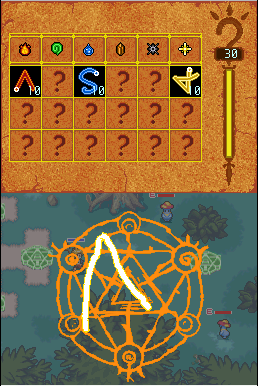
\includegraphics[width=0.4\textwidth]{archivos/lostmagic2.png}
  \caption{Principal mecánica del Lost Magic. Arriba vemos los conjuros aprendidos y abajo en la pantalla táctil podemos dibujarlos.}
  \label{fig:lostmagic1}
\end{figure}

\vspace{0.5cm}

Como muchos RPGs, el jugador también irá subiendo de nivel, mejorando sus características mágicas, y obteniendo objetos.

\clearpage

\begin{figure}[htbp]
\centering
  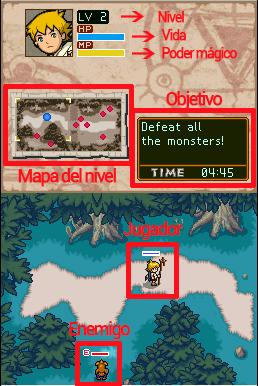
\includegraphics[width=0.4\textwidth]{archivos/lostmagic1.png}
  \caption{Elementos del juego típicos de un RPG.}
  \label{fig:lostmagic2}
\end{figure}

\vspace{0.5cm}

La razón por la que hemos elegido este juego es por estudiar cómo \textbf{implementa el dibujado en tiempo real de los patrones} de hechizos en la pantalla de la NDS y el \textbf{reconocimiento} de estos. Al tratarse de un juego para la \textbf{misma consola} para la que estamos desarrollando y estar desarrollado por una gran empresa como es Taito, podemos hacernos una idea del \textbf{resultado} que podríamos obtener y las limitaciones que existen.

\vspace{1cm}

\subsection{Wario Ware: Touched!}

Wario Ware: Touched!  es un juego basado en \textbf{minijuegos} de la saga Wario Ware que \textbf{Nintendo} desarrolló para la NDS en 2004.

\vspace{0.5cm}

En este juego tendremos distintos \textbf{niveles representados por personajes} tales como Wario, Mona, Kat y Ana, Ashley... En \textbf{cada nivel} debemos pasarnos una \textbf{serie de minijuegos muy cortos en un tiempo determinado} (unos 15 segundos) que suelen ser de dibujar algo en la pantalla táctil, soplar al micrófono, etc. Si no lo logramos, \textbf{perderemos una vida}, lo cual es muy importante pues al pasarnos una serie de minijuegos llegará el \textbf{minijuego de final de nivel} que deberemos completar para completarlo.

\clearpage


\begin{figure}[htbp]
\centering
  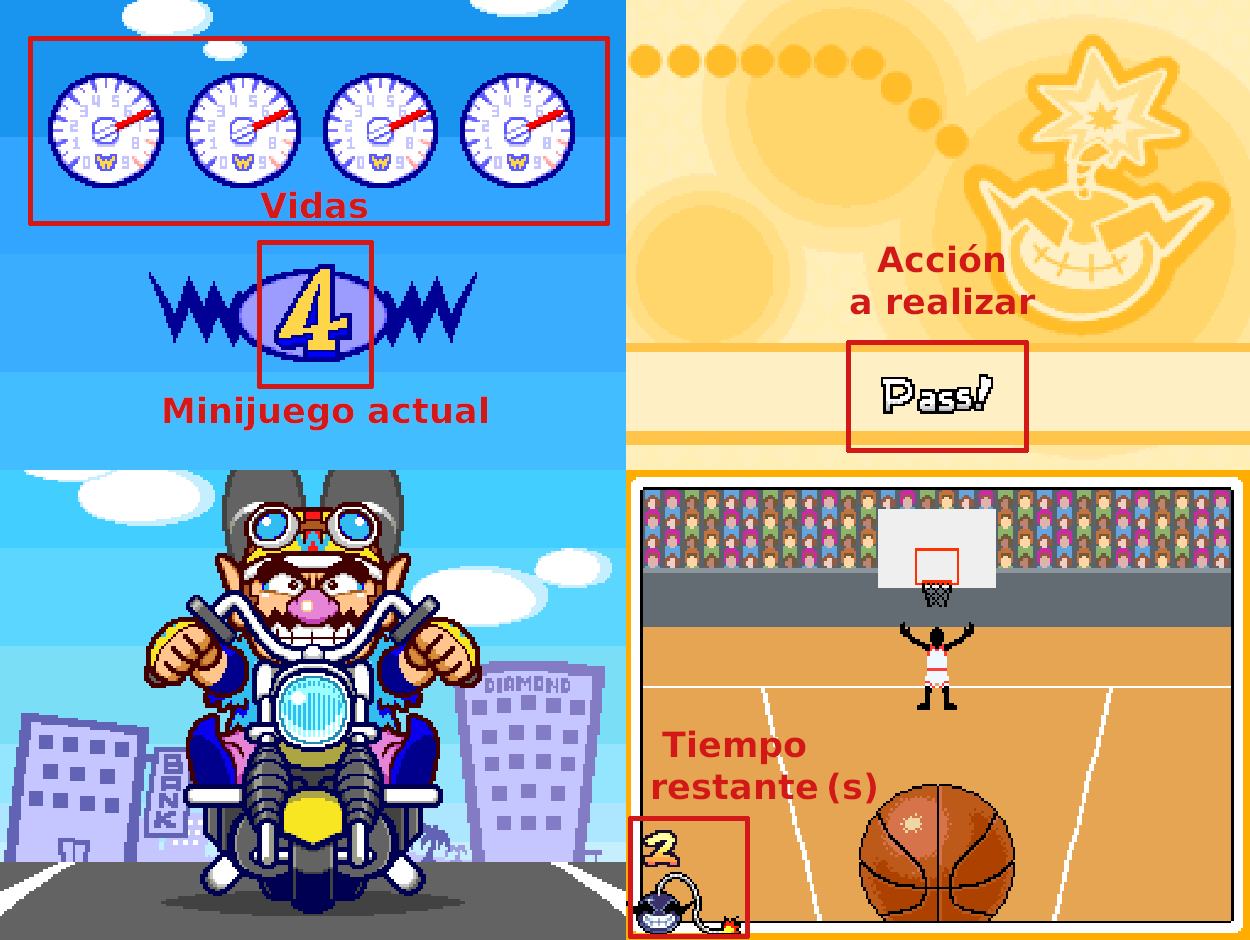
\includegraphics[width=0.6\textwidth]{archivos/wario_ware_level.png}
  \caption{Pantalla de cambio entre minujuegos y minujuego específico de Wario Ware: Touched!.}
  \label{fig:wario_ware_level}
\end{figure}

\vspace{0.5cm}

La razón de escoger este juego como referente es la misma que la de Lost Magic. Me gustaría estudiar cómo es capaz de \textbf{dibujar en tiempo real trazados del usuario} así como gran cantidad de \textit{sprites} y fondos en pantalla que aparecen y desaparecen en cuestión de segundos, \textbf{optimizando así los recursos de la consola}. También, personalmente me gusta mucho el \textbf{estilo del arte} en los \textit{sprites} y diseño de personajes ya que son bastante carismáticos y únicos, y en cierto modo me gustaría inspirarme en ello para poder crear los de este proyecto.

\vspace{1cm}

\chapter{Metodología}

La metodología que se ha usado para llevar a cabo el proyecto se basa en las \textbf{metodologías ágiles} como \textbf{Scrum}.

 \vspace{0.5cm}

Este tipo de metogologías suelen aplicarse en \textbf{proyectos que se realizan en grupo} para así separar bien las tareas, que todos los integrantes puedan trabajar desacopladamente e ir obteniendo resultados lo antes posible. No obstante, este proyecto se trata de un trabajo que se va a realizar únicamente por una persona, pero aún así sigue siendo una buena idea aplicar este tipo de metodologías ya que este es un proyecto donde queremos \textbf{tener un producto lo antes posible}, y que nos permita ir mejorándolo, añadiéndole funcionalidades o características extras que lo mejoren. 

 \vspace{0.5cm}

Así pues, se ha \textbf{adaptado} la metodología Scrum al desarrollo de este videojuego para NDS aplicando un \textbf{desarrollo iterativo}. Al principio, se planificó  una serie de iteraciones teniendo en cuenta el tiempo disponible, asignándoles los objetivos o tareas generales que se debían realizar en éstas. A pesar de que en las metodologías ágiles las iteraciones son de periodos cortos de tiempo, en este caso se decidió ampliar esos tiempos ya que el equipo de trabajo es de únicamente una persona. No obstante las iteraciones se planeó que duraran como máximo un mes.

 \vspace{0.5cm}

Por otro lado, después de cada iteración, se extraía una \textbf{conclusión} del trabajo desarrollado en ésta y se valoraba \textbf{modificar la planificación inicial} si surgía algún problema.

 \vspace{1cm}

\section{Planificación}

A continuación se detallan las iteraciones que se establecieron, con las tareas que se iban a realizar en estas:

\subsection{Iteración 0}

\begin{itemize}
 \item Documentarse sobre cómo desarrollar para NDS. 
 \item Realizar pruebas de dibujado simples que nos den una práctica y conocimiento necesarios para empezar a crear el proyecto.
 \item Analizar los referentes y realizar un diseño del juego.
\end{itemize}

\subsection{Iteración 1 - 4}

\begin{itemize}
 \item Desarrollo del juego, de sus mecánicas y algoritmos necesarios.
 \end{itemize}
 
 \subsection{Iteración 5 - 6}
 
 \begin{itemize}
 \item Mejoras visuales y de retroalimentación para el usuario. 
 \item Realización de pruebas para encontrar fallos tanto en el funcionamiento como en el diseño.

 \end{itemize}
 
  \vspace{0.5cm}
 
 Por último, para llevar un \textbf{seguimiento de la planificación} se ha utilizado la herramienta \textbf{Trello}. Se creó un tablero con la listas de tareas generales para especificar las tareas que el proyecto requería, la lista de iteración actual, para especificar qué tareas se debían realizar en esa iteración, la lista WIP\footnote{WIP: del inglés, \textit{Work In Progress}.}, que contiene las tareas en las que se están trabajando actualmente, y la lista finalizado, que contiene las que ya se han acabado. Además también tiene una lista de problemas, para ir apuntando los inconvenientes que surjan durante el desarrollo y asegurar así que no se quedaban sin resolver.
 
  \vspace{0.5cm}
 
 Se trata de una herramienta muy cómoda, pues de un simple vistazo puedes saber el estado del proyecto, y, además, es muy cómoda de utilizar.

  \vspace{0.5cm}
  
  \begin{figure}[htbp]
\centering
  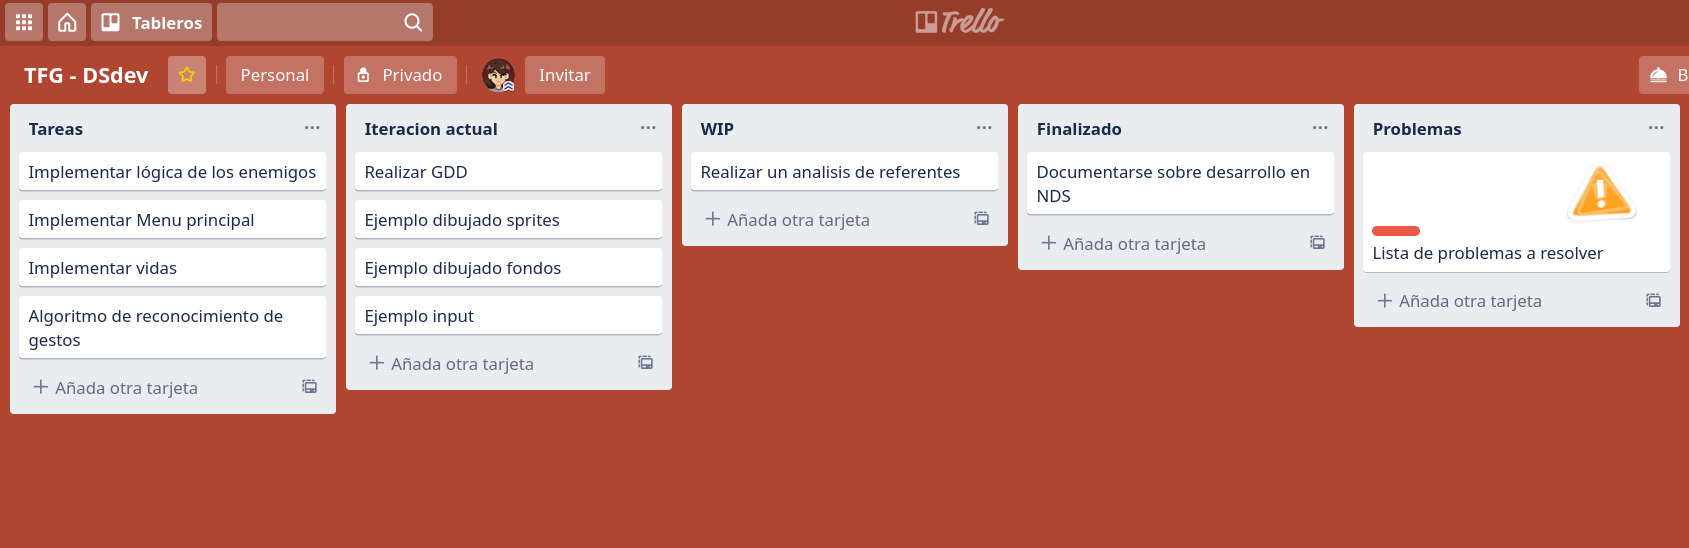
\includegraphics[width=1\textwidth]{archivos/trello.png}
  \caption{Estado del tablero de Trello durante la iteración 0.}
  \label{fig:trello}
\end{figure}

 
\section{Mínimo producto viable}

El diseño realizado en el apartado Diseño del juego está pensado para que, en el mejor de los casos se puedan implementar todas las mecánicas, tipos de enemigos, pantallas, etc. en el tiempo disponible de desarrollo, sin embargo, es poco probable que así sea.

\vspace{0.5cm}

Surgirán problemas, tanto externos como internos, de eso no cabe duda, y no queremos vernos en la situación de estar a pocas semanas de la fecha final y \textbf{solo tener un prototipo}. Es por ello que hay que estar preparado para ese problema y definir una versión simplificada, que siga funcionando como juego y sea un \textbf{producto cerrado} de principio a fin, algo que la gente pueda probar para ver si le gustan las mecánicas o no y a partir de ahí \textbf{trabajar iterativamente} sobre ello añadiéndole las funcionalidades explicadas anteriormente con un \textbf{orden de prioridad}.

\vspace{0.5cm}

Así pues, el mínimo producto que se plantea es el siguiente:

\vspace{0.5cm}

Tendrá un \textbf{único y primer nivel}, donde los enemigos que aparezcan solo tengan \textbf{un patrón} que será al azar entre \textbf{dos tipos distintos} (horizontal y vertical).

\vspace{0.5cm}

Se implementará la \textbf{muerte} del jugador, así como la \textbf{victoria}, de modo que el juego pueda \textbf{rejugarse} tantas veces como se quiera. No obstante, no sería necesario implementar aún las respectivas pantallas de fin de juego y victoria, con volver a la pantalla principal bastaría.

\vspace{0.5cm}

Por último carecería de animaciones y sonido, pues implementar las \textbf{mecánicas} es \textbf{prioritario} frente a perfeccionar lo visual. Sin embargo, sí que se implementará el dibujado del \textbf{rastro del lápiz en la pantalla táctil}, así nos servirá como \textbf{método de depurado} en caso de que el reconocimiento de gestos nos de problemas.

\vspace{0.5cm}

En la siguiente imágen se muestra un mockup de lo que sería el mínimo producto viable:

\vspace{0.5cm}

\begin{figure}[htbp]
\centering
  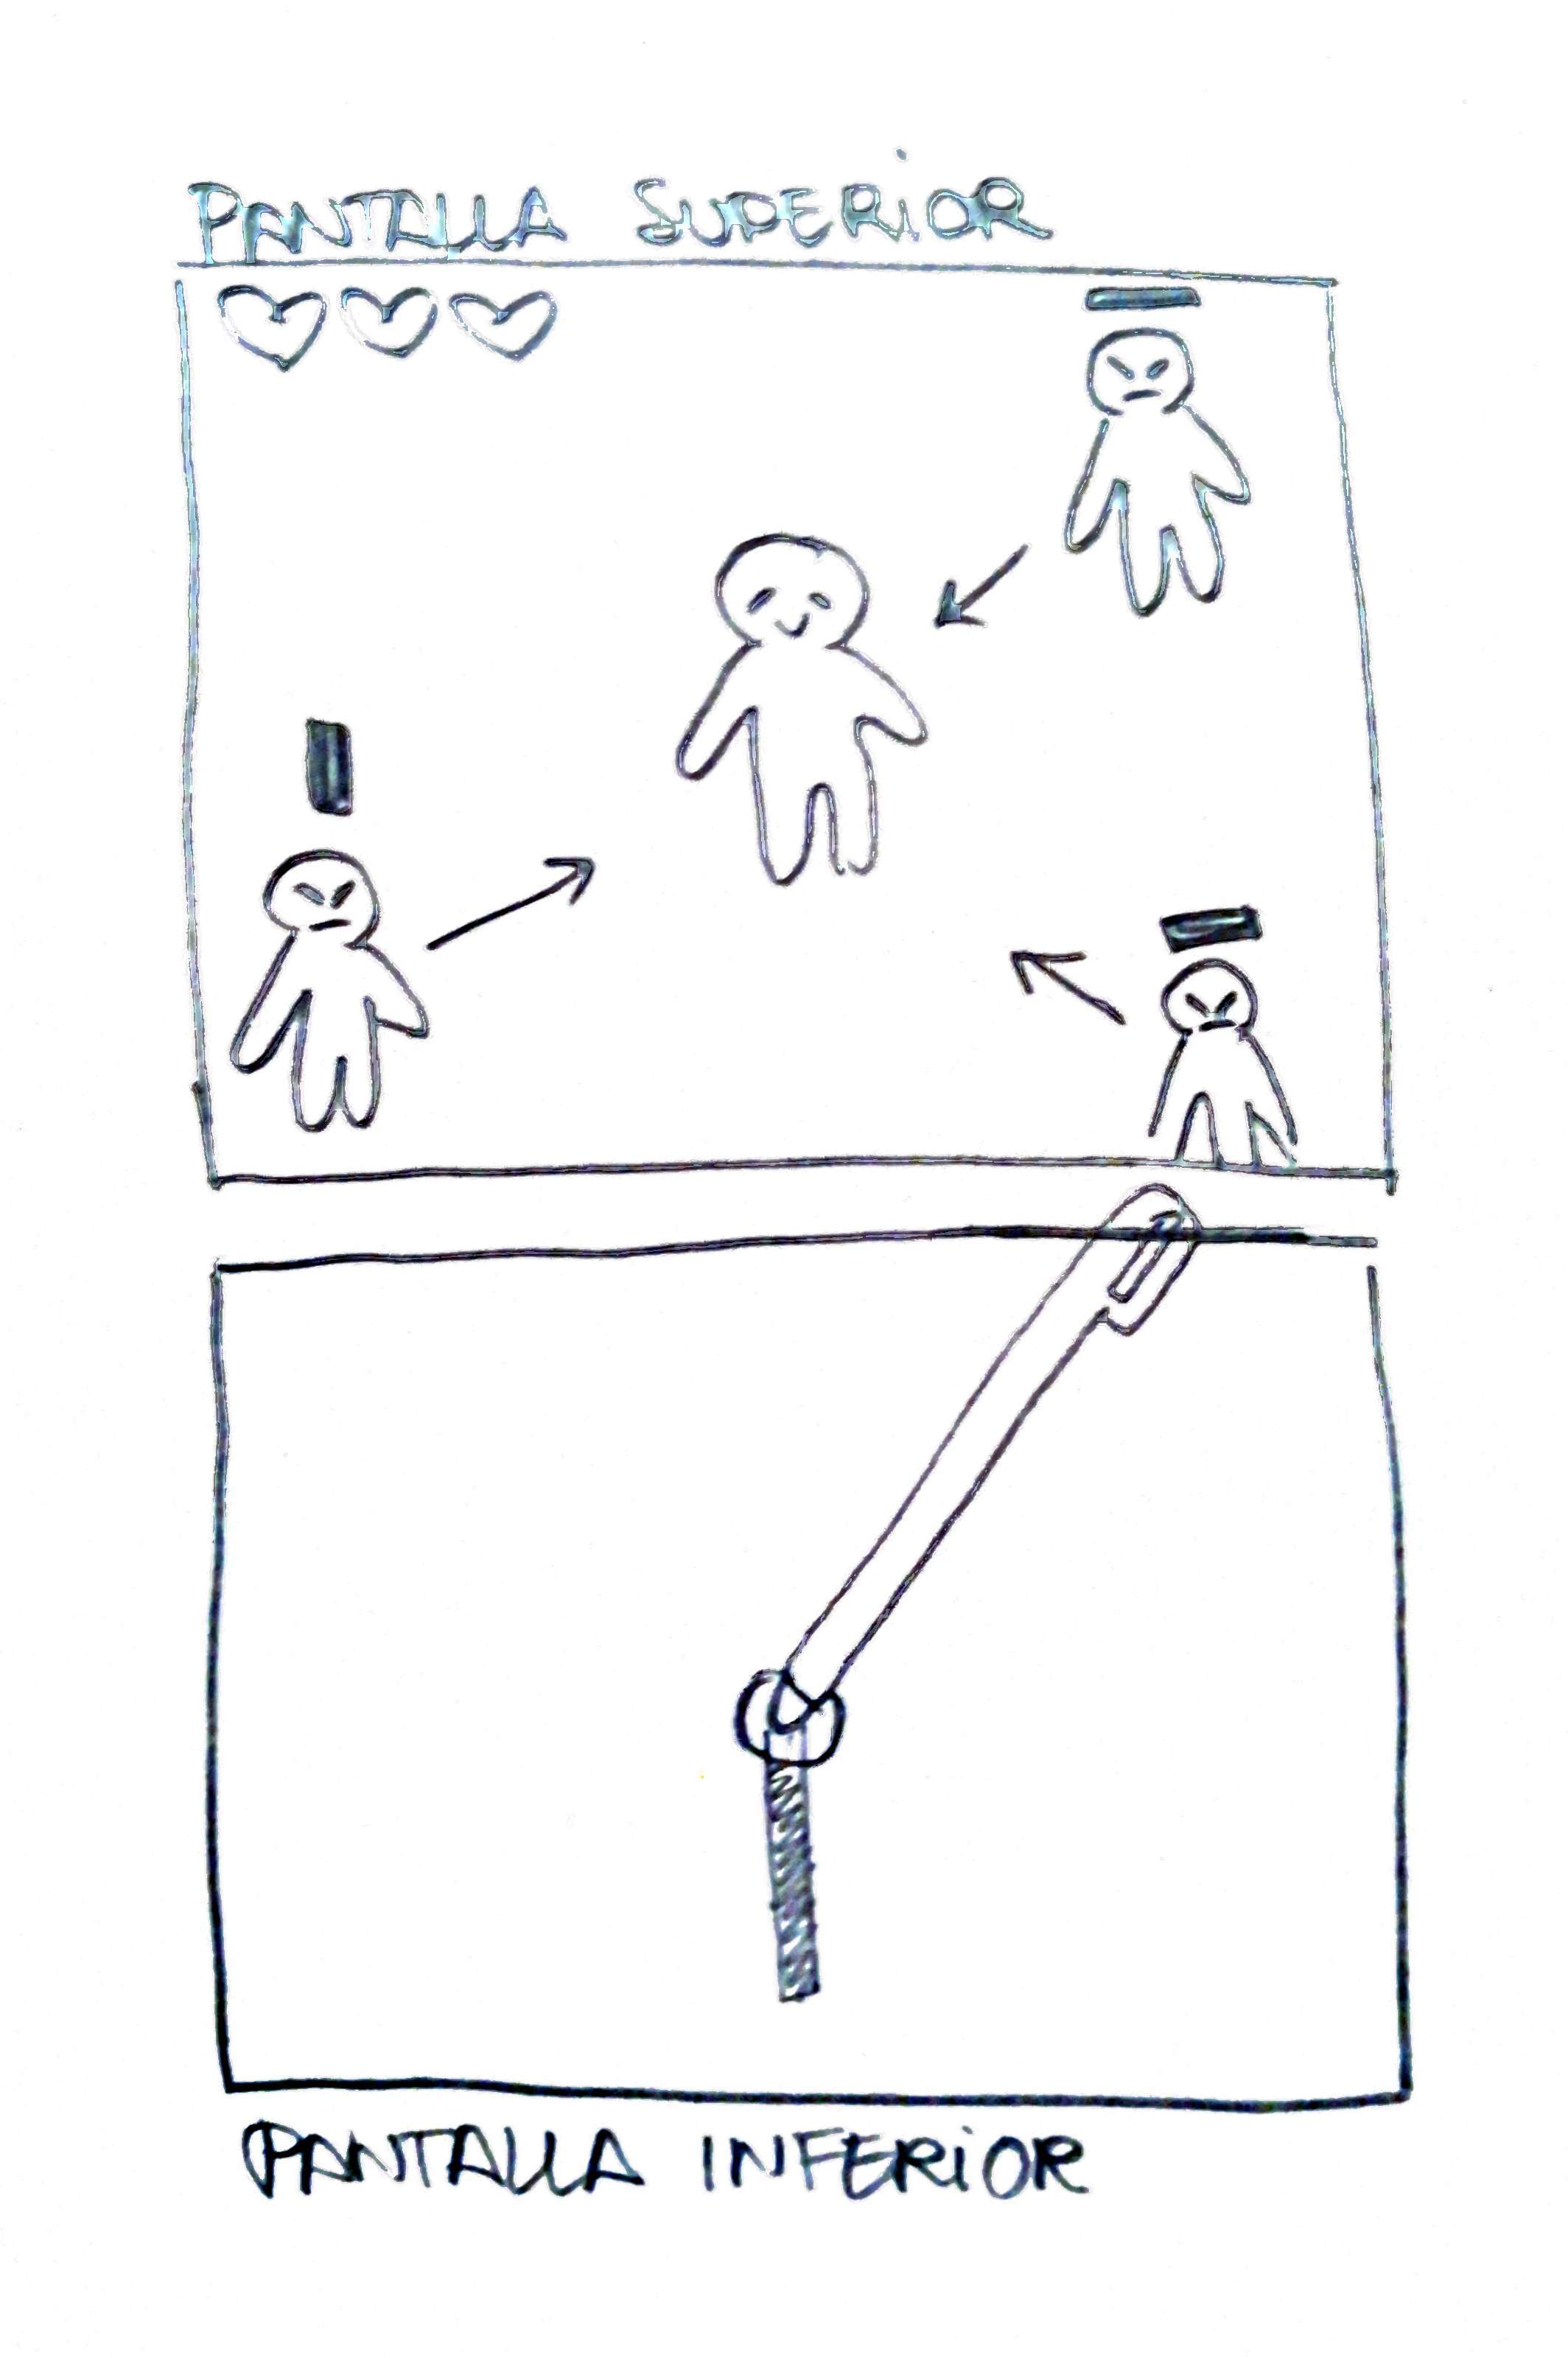
\includegraphics[width=0.4\textwidth]{archivos/minimoprod.jpg}
  \caption{Concepto del mínimo producto viable.}
  \label{fig:minimoprod}
\end{figure}

%%%%%%%%%%%%%%%%%%%%%%%%%%%%%%%%%%%%%%%%%%%%%%%%%%%%%%%%%%%%%%%%%%%%%%%%%
% Plantilla TFG/TFM
% Escuela Politécnica Superior de la Universidad de Alicante
% Realizado por: Jose Manuel Requena Plens
% Contacto: info@jmrplens.com / Telegram:@jmrplens
%%%%%%%%%%%%%%%%%%%%%%%%%%%%%%%%%%%%%%%%%%%%%%%%%%%%%%%%%%%%%%%%%%%%%%%%

\chapter{Objetivos}
\label{objetivos}

El factor común de los objetivos de este estudio es el análisis de los campos acústicos frente a la distancia y la prominencia del campo útil (0 a 50ms) sobre el campo perjudicial (50ms a $\infty$).
Se busca obtener los siguientes puntos:


\paragraph{Validación de modelos}~

Habitualmente los modelos acústicos de recintos son validados únicamente por el valor del tiempo de reverberación, comparando el calculado con el medido experimentalmente, esto aunque es válido no confirma con seguridad que el comportamiento acústico sea similar al recinto real. Por ello, se ha buscado un parámetro más para comparar el modelo con el recinto real y poder confirmar la validez de éste, en concreto se analizan los campos acústicos obteniendo un ecograma para cada receptor y dividiendo temporalmente en dos partes los valores (ver figura \ref{fig:democampos}) para obtener finalmente una pareja de curvas de niveles de presión acústica frente a la distancia a la fuente (ver figura \ref{fig:democamposmultiple}).
\begin{figure}[ht]
    \centering
    \includegraphics[width=\textwidth]{archivos/ecogramaacurva.pdf}
    \caption{Proceso para separar los campos útil y perjudicial a partir de un ecograma. Ejemplo de un receptor a 2 metros de la fuente.}
    \label{fig:democampos}
    \vspace{-0.5cm}%
\end{figure}
\FloatBarrier

\begin{figure}[ht]
    \centering
    \includegraphics[width=0.5\textwidth]{archivos/ecogramaacurvamultiple.pdf}
    \caption{Resultado al separar los campos útil y perjudicial a partir de ecogramas de múltiples receptores a diferentes distancias de la fuente.}
    \label{fig:democamposmultiple}
\end{figure}
\FloatBarrier

Dentro del capítulo de desarrollo en el apartado \textit{validación de modelos} (\ref{validaciondemodelos}) se pueden observar los detalles de esta validación y las opciones para realizarla a través de los programas CATT-Acoustic y EASE. Además de esta validación también es posible comparar parámetros como la claridad o la definición mediante las ecuaciones definidas en el apartado de inteligibilidad (\ref{desarrollointeligibilidad}).

\paragraph{Factores de corrección para el cálculo de campos acústicos}~

Una vez definida en este estudio la \textit{teoría revisada corregida} (\ref{teoriarevisadacorregida}) se tratará de obtener, por medio de medidas en recintos de diferentes tamaños y características, unos coeficientes de corrección para cada uno de ellos. Estos coeficientes se analizarán al detalle para determinar si son coherentes con lo que se espera del comportamiento de los campos acústicos (apartado \ref{comparacioncoef}) y una vez comprobado se buscará una posible relación entre los parámetros del recinto y los factores de corrección para así poder aplicar en otros recintos el cálculo de los campos acústicos sin tener que acudir a mediciones in situ o modelos acústicos.

\paragraph{Desarrollo de herramientas}~

Para la realización de los objetivos anteriores es necesario desarrollar herramientas para analizar y calcular los campos acústicos y coeficientes con el mayor control posible sobre las variables. Las herramientas desarrolladas se basan en el programa Matlab debido a la facilidad para analizar cada una de las variables, realizar regresiones multivariable y desarrollo de interfaces de usuario. Las descripciones de estas herramientas se encuentran en el anexo \ref{anexoprogramas} y se encuentran disponibles en la plataforma GitHub para su análisis y futuras mejoras.

\begin{figure}[ht]
	\centering%
     {\scalefont{0.8}%
    \input{archivos/graficastikz/diagramametodologia}%
    }
    \caption{Diagrama de la metodología aplicada para la validación de modelos.}%
     \label{diagramametodo}%
\end{figure}
\FloatBarrier

\begin{figure}[ht]
	\centering%
     {\scalefont{0.8}%
    \input{archivos/graficastikz/diagramateoria}%
    }
    \caption{Diagrama de los pasos para la obtención de coeficientes y posterior análisis.}%
     \label{diagramateoriarevisada}%
\end{figure}
\FloatBarrier
~




		
%%%%%%%%%%%%%%%%%%%%%%%%%%%%%%%%%%%%%%%%%%%%%%%%%%%%%%%%%%%%%%%%%%%%%%%%
%Desarrollo de un juego para Nintendo DS | Trabajo de Fin de Grado
% Escuela Politécnica Superior de la Universidad de Alicante
% Realizado por: Carla Maciá Díez
% Contacto: carlamd1997@hotmail.com / cmd23@alu.ua.es
%%%%%%%%%%%%%%%%%%%%%%%%%%%%%%%%%%%%%%%%%%%%%%%%%%%%%%%%%%%%%%%%%%%%%%%%

\chapter{Diseño del juego (Game Design Document)} 

\subsection{Características}

\begin{itemize}
    \item \textbf{Título:} Touch \& Brush.
    \item \textbf{Plataforma:} Familia de consolas Nintendo DS.
    \item \textbf{Genero:} Agilidad mental.
    \item \textbf{Audiencia:} Todas las edades.
    \item \textbf{Idioma:} Inglés.
\end{itemize}

\vspace{1cm}


\subsection{Historia}

Un día cualquiera en un \textbf{museo de arte tradicional} sucedió una catástrofe. Un malvado pincel robó toda la pintura de los \textbf{cuadros} de la exposición haciendo que estos se volviesen \textbf{furiosos}, se separasen de las paredes que los sostenían y empezaran a atacar a la gente.

\vspace{0.5cm}


\textbf{Cherry}, una pequeña niña que disfrutaba de una agradable excursión al museo ese día con su clase, al ver la situación de pánico decide actuar. Es entonces cuando se encuentra con otro pincel, llamado \textbf{Celio}, que le asegura a la chica que la única manera de devolver los cuadros a la normalidad es pintarles lo que ellos quieran. Así pues, Cherry y Celio deciden trabajar juntos para salvar el museo.

\vspace{1cm}


\subsection{Ambientación y estilo}

Al tratarse de un juego 2D para la consola Nintendo DS, el estilo que adoptarán los escenarios y personajes de Touch \& Brush será \textbf{pixelart\footnote{Estilo de arte digital que trabaja con las imágenes a nivel de pixel.} y  cartoon\footnote{Estilo de dibujo y estilización de personajes de personajes con proporciones irreales de tal manera que llega incluso a tener un carácter humorístico y simpático.}}, ya que el tamaño de nuestra pantalla y sprites es reducido.

\vspace{0.5cm}

El juego se desarrolla en el espacio cerrado de un museo de arte, así que el fondo principal donde se desarrolla el gameplay se trata de una de sus salas. Esta misma poseerá las características más típicas de un museo de arte, como puede ser un reluciente parqué, una ténue iluminación con puntos de luz hacia la pared donde deberían ir los cuadros y un fondo azul oscuro para que los sprites y elementos por encima de éste resalten sin problema.

\vspace{0.5cm}

\begin{figure}[htbp]
\centering
  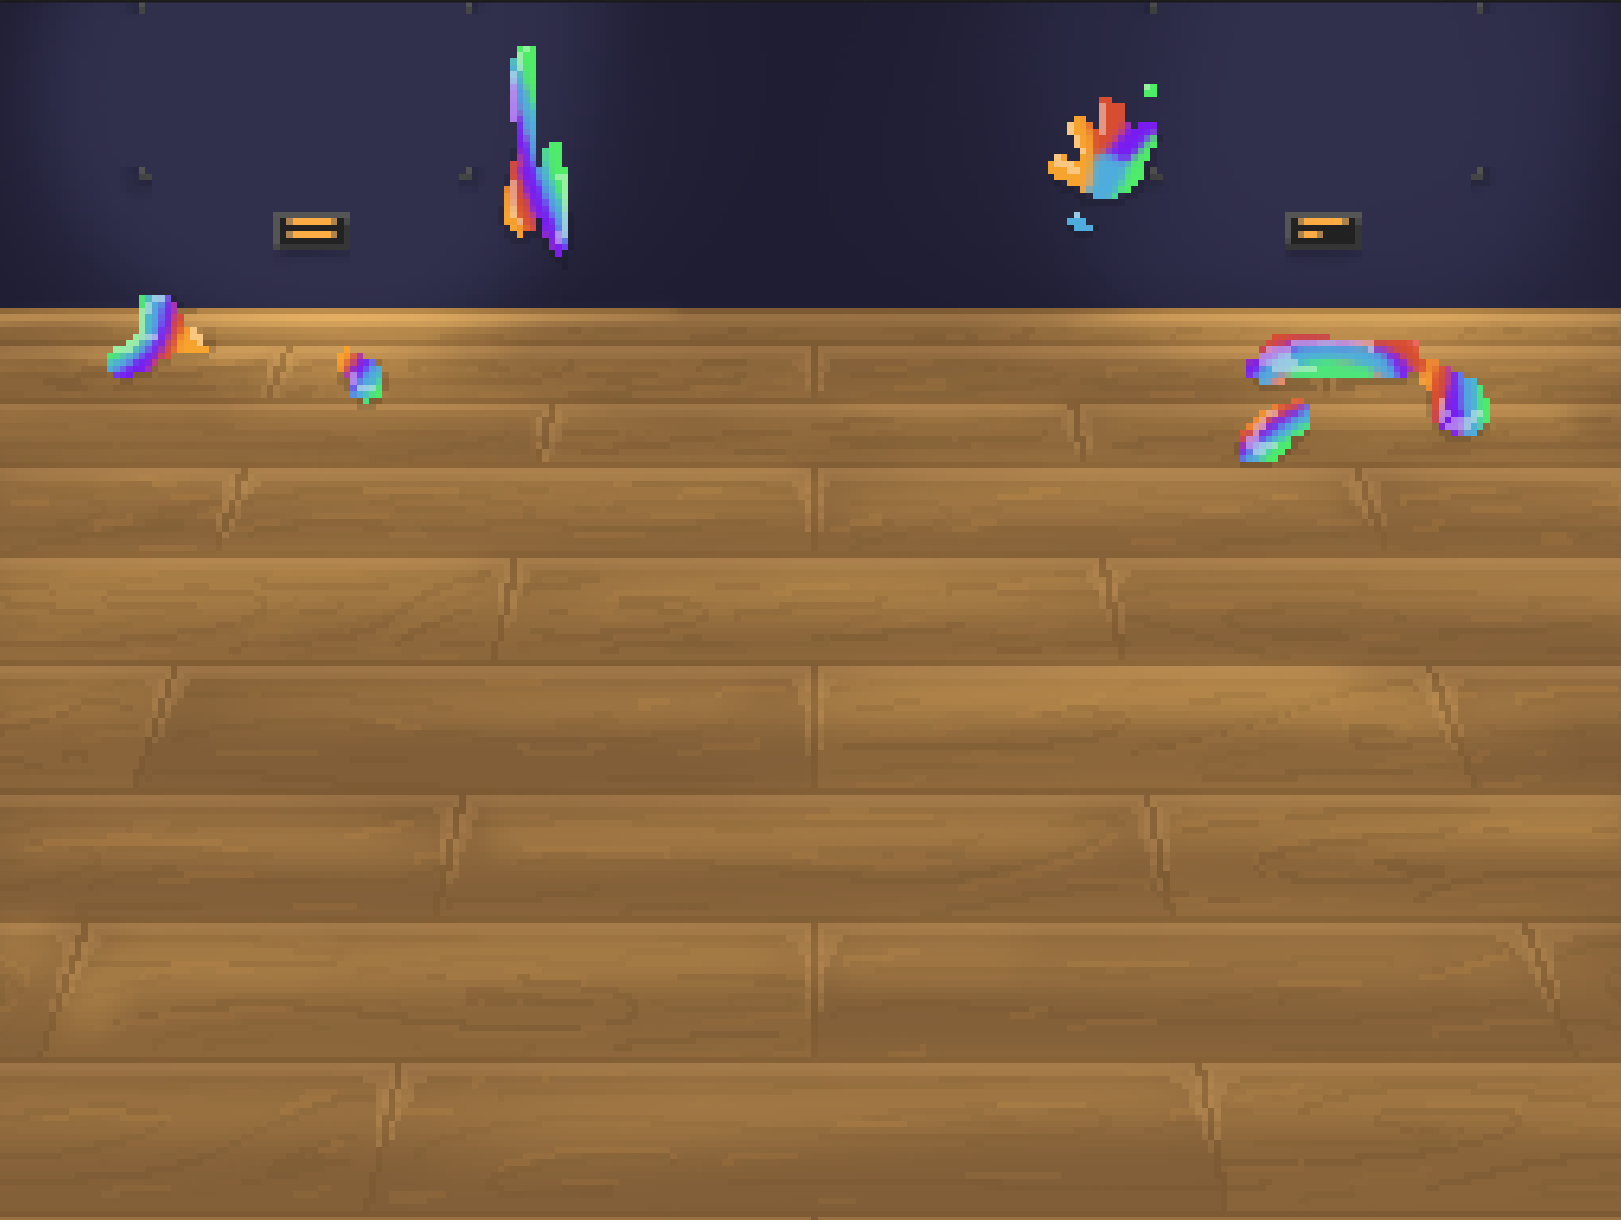
\includegraphics[width=0.5\textwidth]{archivos/bg.png}
  \caption{Fondo de la pantalla de juego que representa la sala de un museo vacía y destrozada.}
  \label{fig:bg_museum}
\end{figure}

\vspace{0.5cm}

Tanto la protagonista como los enemigos tendrán características desproporcionadas tales como gran cabeza, ojos y extremidades, típicas de la estética cartoon. Además, al tratarse de una historia de fantasía y magia, los sprites del juego poseerán \textbf{gran variedad de colores} y bastante saturados, para destacar sobre el fondo y llamar la atención del jugador.



\begin{figure}[htbp]
\centering
  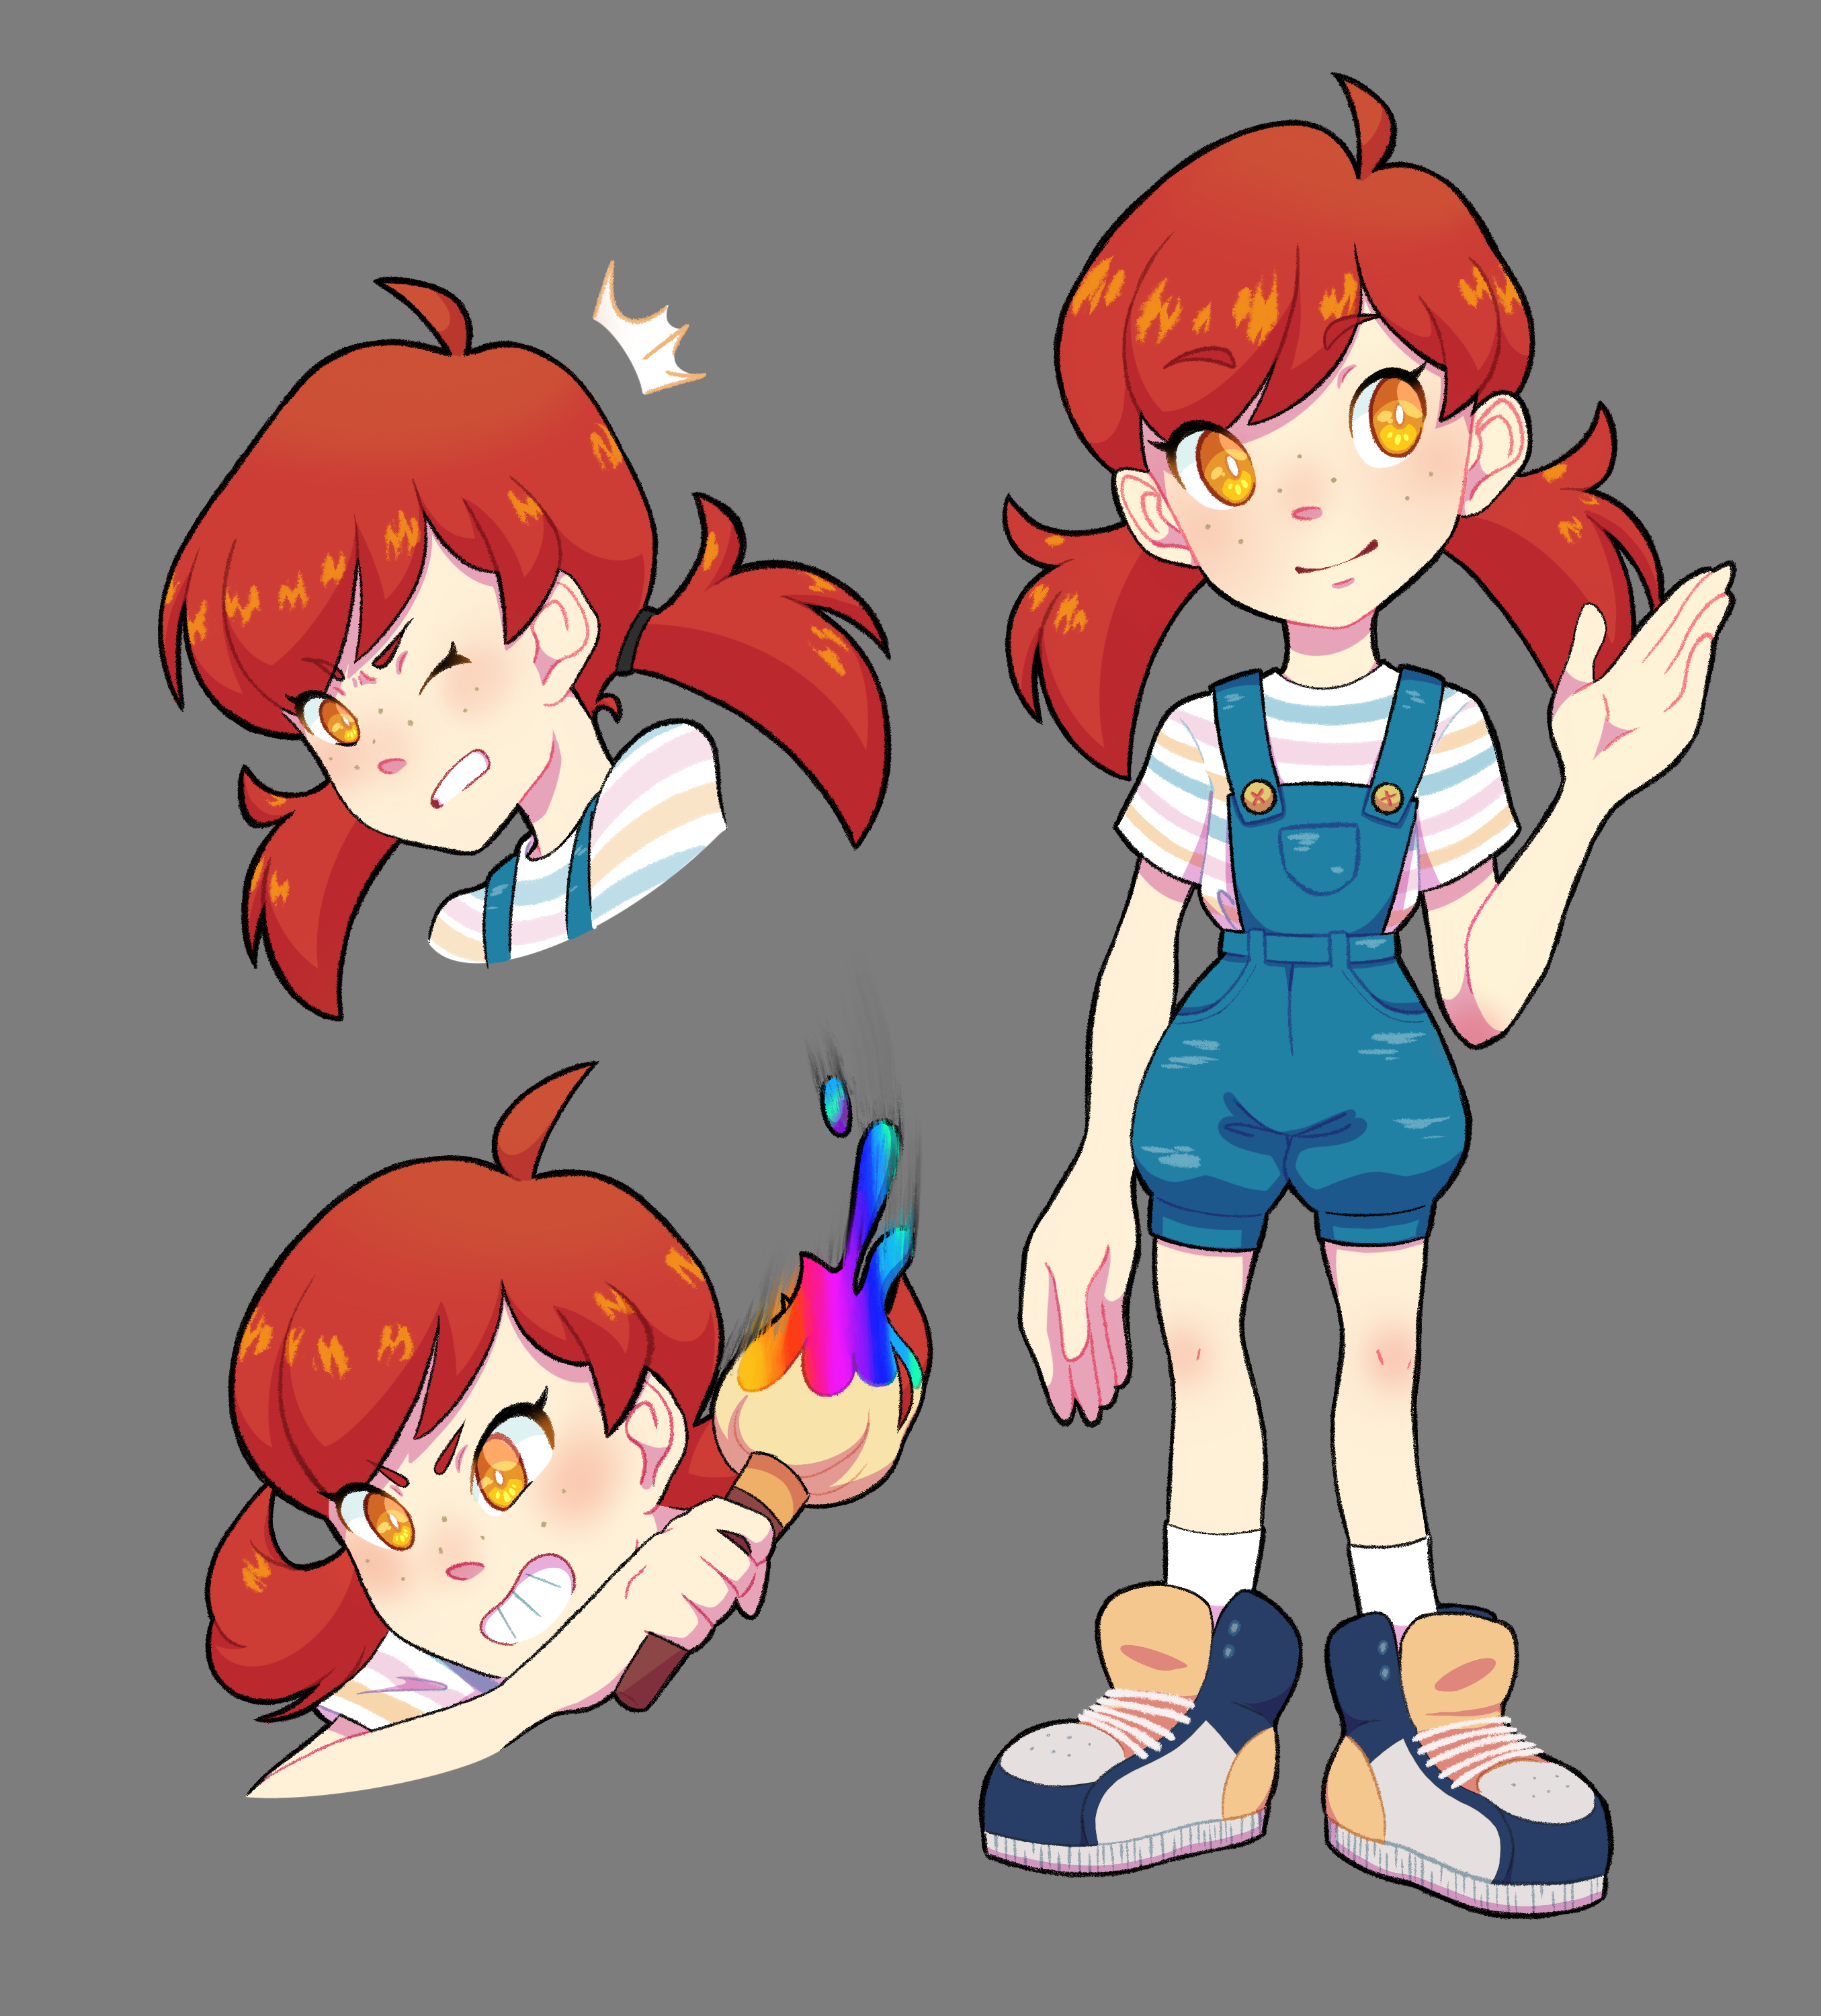
\includegraphics[width=0.45\textwidth]{archivos/cherry.png}
  \caption{Concept art de Cherry, la protagonista del juego, los cuadros.}
  \label{fig:cherry}
\end{figure}

\vspace{0.5cm}

Un toque que posee la ambientación Touch \& Brush y que ayuda a \textbf{unificar el estilo visual} de todo el producto es el uso de \textbf{manchas de pintura de color arcoiris} tratando de simular una pintura mágica. El uso de este recurso se utiliza en diversas ocasiones como por ejemplo, en el pincel Celio, en el logo del juego, en el texto de la pantalla del título y en la mecánica de dibujar en la pantalla táctil y en el propio fondo del museo. Por último, a pesar de que para los gráficos no usaremos una paleta de colores específica, sino más bien todos los que nos permita el hardware, lo que sí haremos será usar el mismo tono lila para hacer las sombras de sprites y fondos. Esto ayudará a cohesionar todos los gráficos y dotar al juego de una consistencia visual.

\vspace{0.5cm}

\begin{figure}[htbp]
\centering
  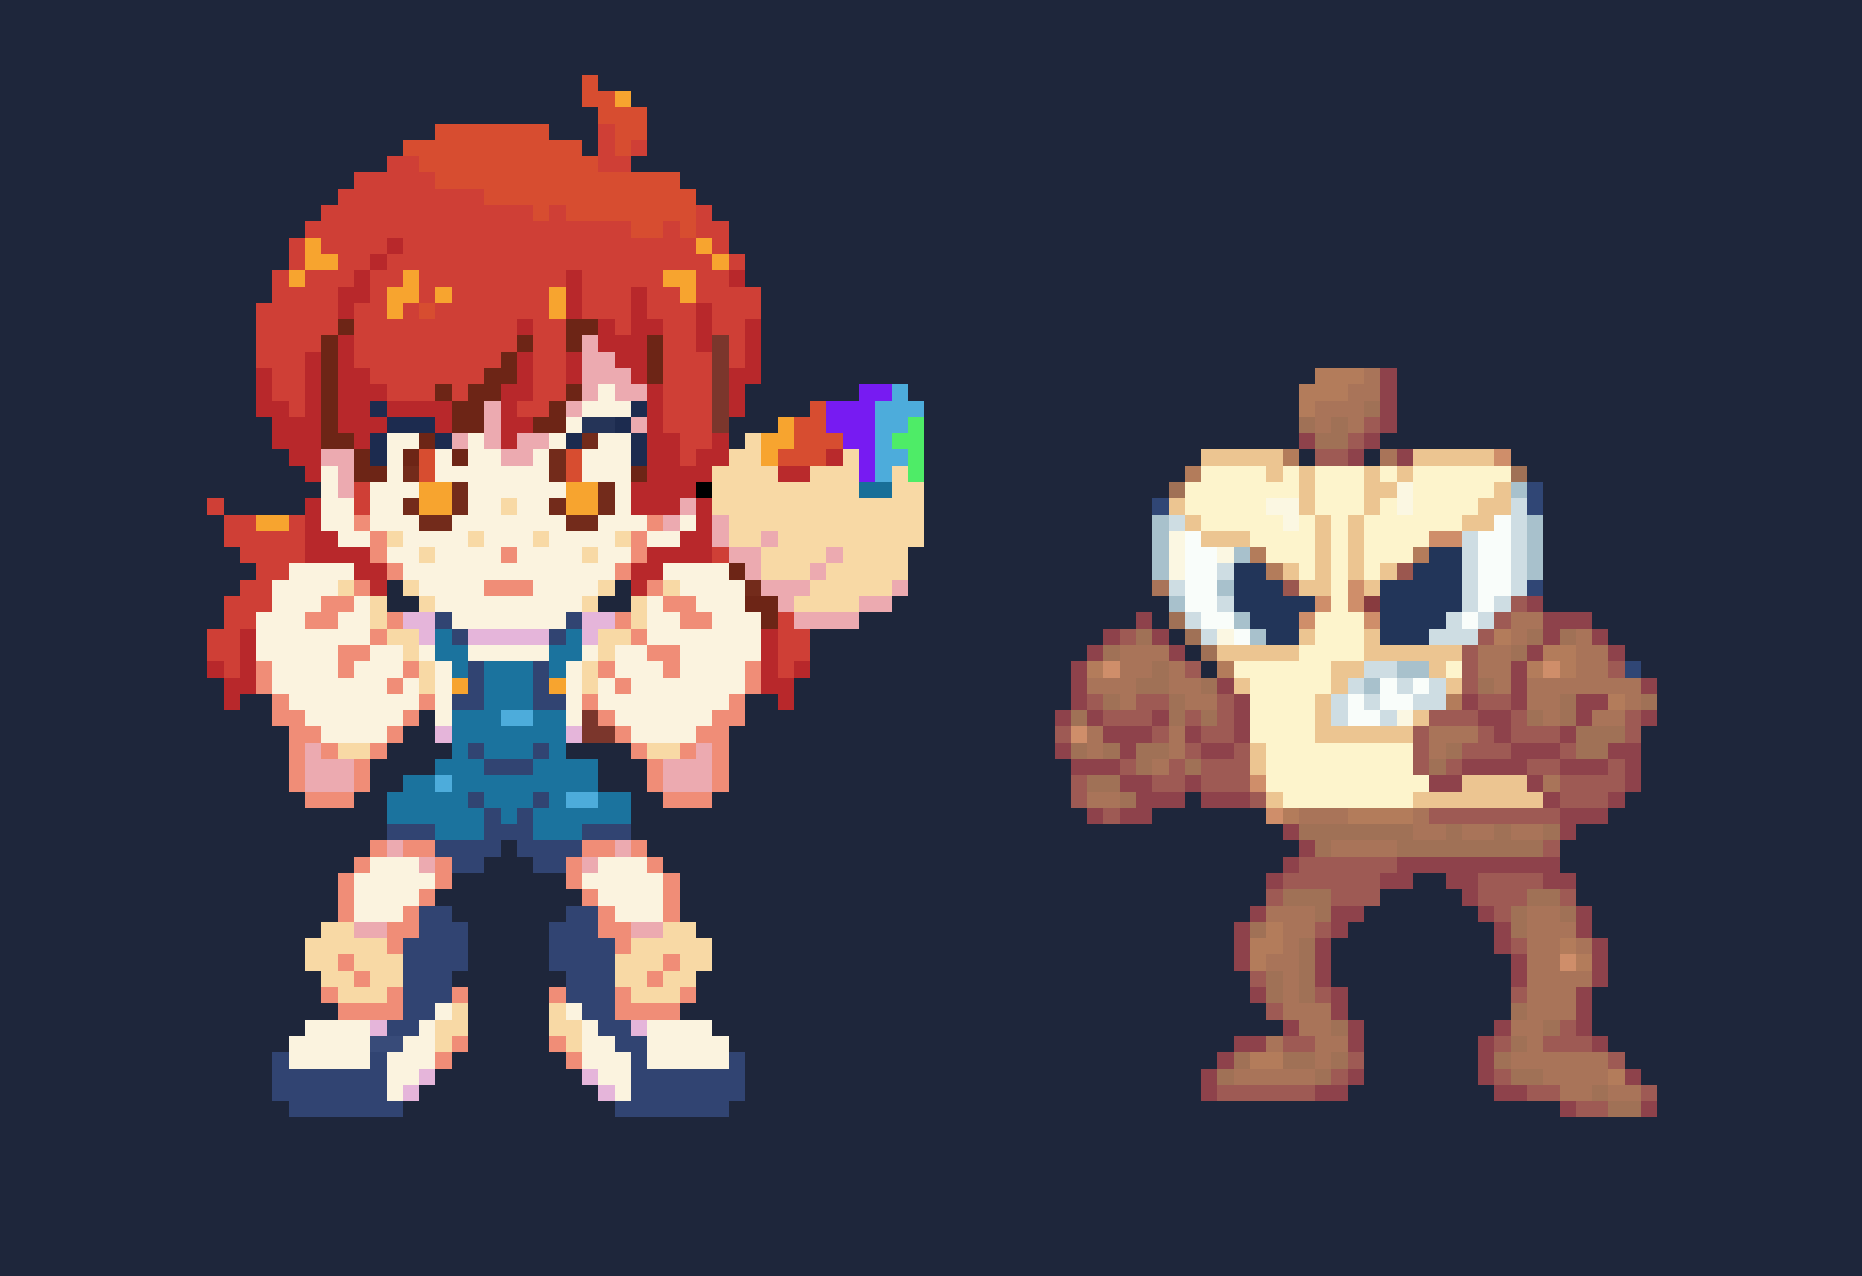
\includegraphics[width=0.5\textwidth]{archivos/sprites.png}
  \caption{Sprites de Cherry y los principales enemigos.}
  \label{fig:sprites_gdd}
\end{figure}

\vspace{1cm}


\subsection{Jugabilidad y mecánicas}

Para \textbf{progresar} en los niveles de Touch \& Brush, el jugador deberá ir \textbf{dibujando el patrón} o conjunto de patrones que los \textbf{enemigos} poseen encima de ellos antes de que éstos lleguen hasta él. El jugador se encontrará en el \textbf{centro superior de la pantalla} y los enemigos aparecerán por los bordes y, al \textbf{alcanzarle}, le \textbf{quitarán una vida}. Este mismo poseerá \textbf{6 vidas} que podrá consultar en todo momento ya que se visualizarán en un \textbf{contador de vidas} en la parte superior izquierda de la pantalla.

\vspace{0.5cm}

Como \textbf{algunos enemigos se moverán más lento que otros}, el reto del jugador es poder \textbf{decidir rápidamente qué patrones dibujar y en qué orden} para avanzar al siguiente nivel con el mayor número de vidas posibles. Además, si somos capaces de \textbf{concatenar varios patrones correctos seguidos} aumentará nuestra \textbf{puntuación}, también visible en cualquier momento en la parte superior derecha de la pantalla.

\vspace{0.5cm}

Por otro lado, si nos encontramos en un nivel de una dificultad superior y hemos perdido más de la mitad de nuestra vida, aparecerá un \textbf{aliado} con un \textbf{patrón de corazón}. Si lo dibujamos correctamente nos aumentará la vida en una unidad.

\vspace{0.5cm}

Al llegar al último nivel encontraremos al \textbf{jefe final}, que debemos derrotar de manera similar a los enemigos normales pero con una serie de fases. Su comportamiento se explicará detalladamente en el apartado de Enemigos.

\vspace{1cm}

\subsection{NPCs}

Dentro del juego distinguiremos tres tipos de NPCs, siendo dos de estos enemigos y uno de ellos un aliado. A continuación se detalla cada uno en profundidad.

\subsubsection{Enemigos comunes}

Como hemos comentado, los enemigos comunes del juego se tratan de los cuadros del museo, que al haberles sido arrebatada su pintura han cobrado vida y se han vuelto furiosos.

\vspace{0.5cm}

Este es el único tipo de enemigo que habrá en los niveles normales del juego y su comportamiento siempre será el mismo: \textbf{ir hacia el jugador} y al alcanzarle le quitará vida. Sin embargo, entre varios enemigos existirán diferencias como por ejemplo la \textbf{velocidad} a la que se mueven, el \textbf{tipo de patrón} que debe dibujar el jugador para matarlos y la\textbf{ posición} desde la que aparecen. Estas características se comentarán más adelante en el apartado de niveles.

\vspace{0.5cm}

Los enemigos podrán aparecer con un patrón de entre \textbf{tres} posibles, los cuales se muestran en la siguiente figura. Se tratan de una l\textbf{ínea horizontal, una línea vertical y un triángulo}. Estos patrones además están representados con \textbf{distintos colores} cada uno para que al usuario, a la hora de visualizarlos en el juego, le sea más fácil distinguirlos.

\vspace{0.5cm}

\begin{figure}[htbp]
\centering
  
\includegraphics[width=0.5\textwidth]{archivos/patterns.png}
  \caption{Tipos de patrones con los que pueden aparecer los enemigos.}
  \label{fig:patterns_enemies}
\end{figure}

\vspace{0.5cm}

\subsubsection{Aliado}

Este NPC tiene la misma apariencia que un enemigo normal, pues también se trata de un cuadro del museo. Sin embargo, \textbf{no es agresivo}, de hecho es beneficioso para el jugador. Su patrón será un dibujo con forma de corazón y si el usuario consigue dibujarlo cuando este aparezca en un nivel, \textbf{aumentará su vida} en una unidad.

\vspace{0.5cm}

Ahora bien, tanto su aparición como su comportamiento no serán igual que los enemigos normales. Este aliado solo aparecerá \textbf{una vez por nivel}, siempre a partir del nivel 3 y siempre que nuestra vida sea igual o inferior a la mitad. Además, no correrá hacia el jugador, sino que aparecerá desde el borde izquierdo de la pantalla y \textbf{avanzará en línea recta hasta la mitad de la pantalla}, donde se detendrá.

\vspace{0.5cm}

\begin{figure}[htbp]
\centering
  
\includegraphics[width=0.3\textwidth]{archivos/heart.png}
  \caption{Tipos de patrones con los que pueden aparecer los enemigos.}
  \label{fig:patterns_heart}
\end{figure}

\vspace{0.5cm}

\subsubsection{Jefe}

Este enemigo se trata del jefe final del juego, el cual representa al \textbf{cuadro más prestigioso} y valorado del museo. En cuanto a su apariencia, es igual que los enemigos normales pero de mayor tamaño, ojos rojizos y porta una corona de rey.

\vspace{0.5cm}

Se podrá encontrar después de haber superado el último nivel y su comportamiento será distinto. En primer lugar, se encontrará en la parte derecha de la pantalla, avanzando hacia la izquierda donde se encuentra el jugador. También, su daño será mayor, quitando de un solo golpe 2 corazones. 

\vspace{0.5cm}

La forma en la que debemos matarlo también será diferente a los demás enemigos. Su comportamiento estará dividido en \textbf{3 fases}, y en cada una de ellas generará una \textbf{secuencia de 5 patrones} que el jugador deberá dibujar \textbf{en orden} mientras dicho jefe se va moviendo a una velocidad concreta hacia este. Si el jugador lo logra, el jefe volverá a su posición inicial, pasando a la siguiente fase, donde aumentará su velocidad y la secuencia de patrones volverá a generarse.

\vspace{0.5cm}

\begin{figure}[htbp]
\centering
  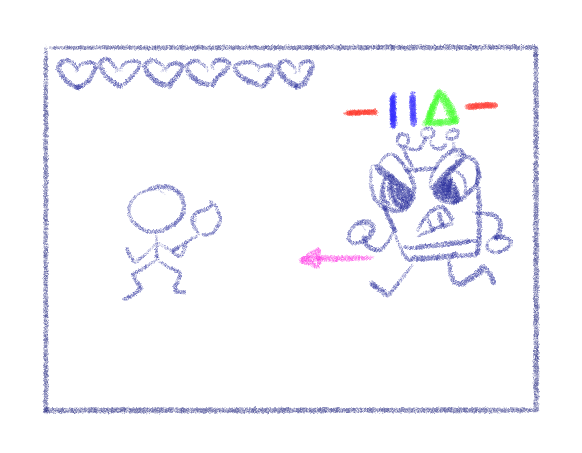
\includegraphics[width=0.5\textwidth]{archivos/mockup_boss.png}
  \caption{Mockup del enfrentamiento con el jefe.}
  \label{fig:mockup_boss}
\end{figure}

\vspace{1cm}

\subsection{Niveles}

El juego constará de \textbf{4 niveles normales} y \textbf{un nivel de jefe final}.

\vspace{0.5cm}

En cuanto a los niveles normales, visualmente no serán muy distintos entre sí, pero sí que hay \textbf{5 parámetros} que podemos ajustar para dotar a los niveles de Touch \& Brush de una curva de complejidad y aprendizaje interesantes.

\vspace{0.5cm}

En primer lugar, tenemos el \textbf{tiempo} que transcurre entre la aparición de enemigos. A medida que avancemos en los niveles, este tiempo se irá reduciendo para que aparezcan enemigos con más frecuencia y el jugador deba dibujar los patrones más rápido.

\vspace{0.5cm}

Después, tenemos la \textbf{posición} desde la que aparecen los enemigos y la \textbf{velocidad} a la que se mueven. Al encontrarse el jugador en el centro de la pantalla, los enemigos podrán salir desde 6 posiciones distintas y dirigirse hacia él. Estas posiciones son: esquinas superiores derecha e izquierda, centro derecha e izquierda y esquinas inferiores derecha e izquierda. En cuanto a la velocidad, es interesante que algunos enemigos sean capaces de moverse más rápido que otros para despistar al jugador. Por ejemplo, si sale un enemigo desde un lado a una velocidad lenta el jugador se fijará en ese e intentará derrotarlo, pero entonces es cuando aparece un enemigo que se mueve más rápido, le alcanza antes de que pueda darse cuenta o reaccionar y le quita una vida.

\clearpage

\begin{figure}[htbp]
\centering
  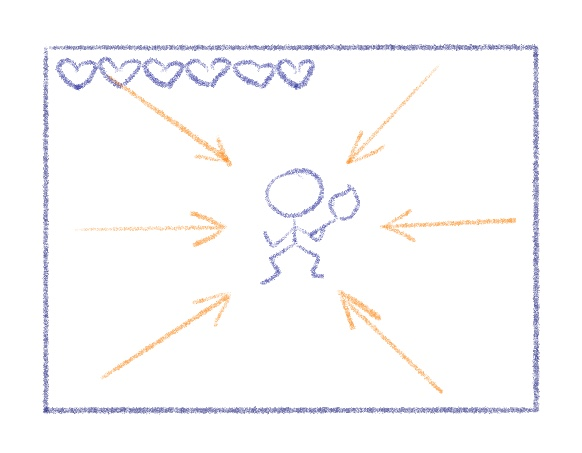
\includegraphics[width=0.4\textwidth]{archivos/pos_enemies.jpg}
  \caption{Posiciones iniciales desde las que pueden aparecer enemigos.}
  \label{fig:pos_enemies}
\end{figure}

Por otro lado tenemos el \textbf{número de enemigos que debemos derrotar} para pasar al siguiente nivel, que irá aumentando según avancemos. Y por último, tenemos la \textbf{complejidad de los patrones} de los enemigos. Es bastante más fácil de dibujar una línea recta que un triángulo, así que los primeros niveles comenzarán con esos patrones más simples y a medida que avancemos se incorporarán los más complejos.

\vspace{0.5cm}

Así pues, una vez explicado esto, los 4 niveles de Touch \& Brush tendrían las siguientes características:

\begin{itemize}
  \item \textbf{Nivel 1:} Enemigos lentos que únicamente aparecen por los laterales centrales de la pantalla, moviendose lento y sus patrones serán la línea horizontal y vertical. Será necesario derrotar aun total de 6 enemigos para pasar al siguiente nivel y la frecuencia con la que estos aparecen será la más baja.
  
    \item \textbf{Nivel 2:} En este nivel se incorporan los enemigos que salen desde las esquinas superiores e inferiores, llevando estos una velocidad mayor. Además, el número de enemigos a derrotar aumenta a 10 así como aumenta también la frecuencia con la que éstos aparecen.
    
    
    \item \textbf{Nivel 3:} Se mantienen las mismas posiciones y velocidades de los enemigos, así como sus patrones. Aumenta el número de enemigos que derrotar a 13 y también lo hace la frecuencia con la que éstos aparecen. Se incorpora el aliado que te permite recuperar vida.
    
    
    \item \textbf{Nivel 4:} Nuevamente, aumenta el número de enemigs que derrotar a 16 y la frecuencia con la que aparecen. Además también aparecen los enemigos con patrón de triángulo.
    
\end{itemize}

\subsection{Controles}

En cuanto a los controles, al tratarse de un juego para una consola con pantalla táctil la gran mayoría de interacciones tanto para el \textbf{gameplay principal} como la \textbf{selección de opciones en los menús} se harán mediante esta. No obstante, cabe destacar que para \textbf{abrir el menú de pausa} se pulsará el botón \textbf{START}.

\subsection{Estados del juego}
 Aquí veremos un resumen de todos los estados del juego, así como el flujo entre ellos para que a la hora de desarrollar tengamos en cuenta desde qué estados se puede llegar a uno en concreto. 
 
 \vspace{0.5cm}
 
 En la siguiente imágen se puede observar dicho resumen, y más adelante veremos las pantallas que se corresponden con cada estado.
 
  \vspace{0.5cm}
 
 \begin{figure}[htbp]
\centering
  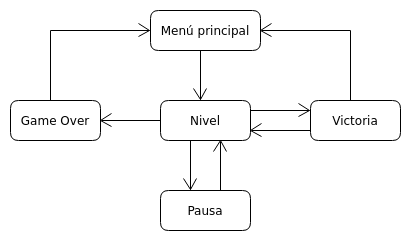
\includegraphics[width=0.5\textwidth]{archivos/diagramaflujo.png}
  \caption{Diagrama de flujo entre estados}
  \label{fig:diagflujo}
\end{figure}

 \vspace{0.5cm}

Al inciar el juego se cargará el \textbf{menú principal}, que nos dará la opción de empezar a jugar desde el primer nivel ya que no habrá guardado de partida. Si completamos un nivel, pasaremos al estado de \textbf{victoria}, que nos mostrará un mensaje de que hemos completado el nivel y nos dará la opción tanto de volver a jugar ese nivel, continuar al siguiente o volver al menú principal.

 \vspace{0.5cm}

Por otro lado, si mientras jugamos perdemos, independientemente del nivel en el que nos encontrasemos pasaremos al estado de \textbf{fin de partida}, que nos mostrará un mensaje de que hemos muerto, la puntuación obtenida y únicamente nos permitirá volver al menú principal.

 \vspace{0.5cm}

Por último, mientras estemos jugando a cualquier nivel podremos cambiar al \textbf{estado de pausa} si deseamos dejar en espera nuestro juego y así mismo desde este menú de pausa podremos volver al estado donde dejamos la partida.

 \vspace{0.5cm}

\subsection{Pantallas}

A continuación se muestran una serie de \textbf{bocetos de pantallas} asociadas a los distintos estados del juego, así como también los elementos visuales que estos poseen, qué información nos dan y si son interactuables.

 \vspace{0.5cm}
 
 En primer lugar, la pantalla del menú principal. En ella no habrán muchos elementos, teniendo en la pantalla superior el logo del juego y, en la inferior un mensaje que nos indicará que debemos tocar la pantalla para comenzar a jugar. Además, en esta misma pantalla también se mostrará el nombre del autor del juego.
 
  \begin{figure}[htbp]
\centering
  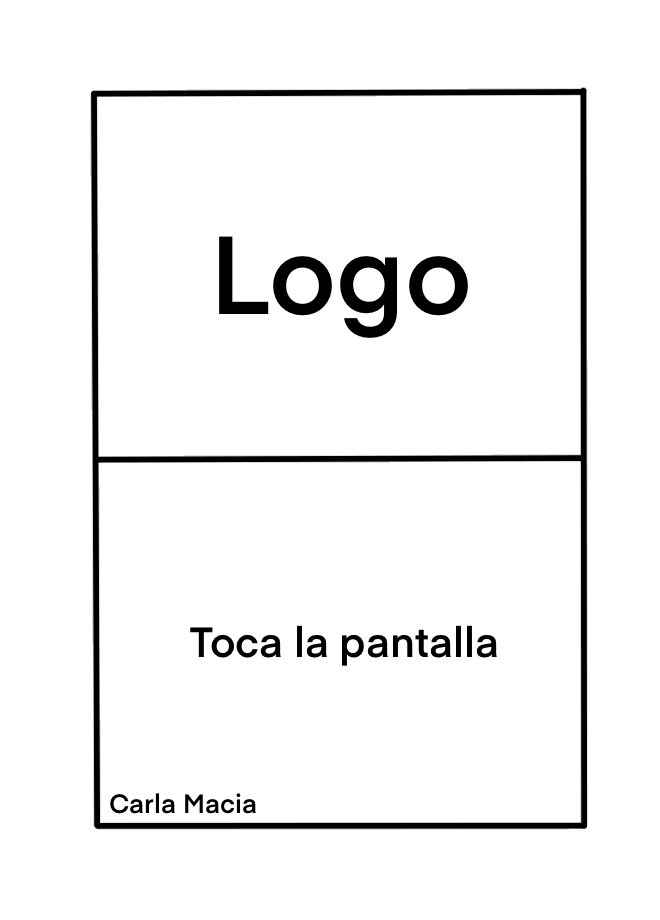
\includegraphics[width=0.3\textwidth]{archivos/mockup_title.png}
  \caption{Mockup de la pantalla de título}
  \label{fig:mockup_title}
\end{figure}

 \vspace{0.5cm}
 
 Por otro lado tenemos la pantalla de nivel, siendo esta donde el jugador más tiempo pasará y más información le aportará. En la pantalla superior, haciendo uso de sprites se podrán visualizar los enemigos moviendose por la pantalla, el jugador y la vida de éste mismo. Además, en la parte derecha superior tendremos un contador que nos indicará nuestra puntuación y se irá actualizando mientras jugamos.
 
 \vspace{0.5cm}
 
 En la pantalla inferior es donde el jugador irá dibujando los patrones, por ello mediante un fondo simularemos una especie de lienzo y cuando el jugador esté tocando la pantalla táctil iremos dibujando el trazo que éste realiza.
 
 \clearpage
 
   \begin{figure}[htbp]
\centering
  \includegraphics[width=0.3\textwidth]{archivos/mockup_game.png}
  \caption{Mockup del juego}
  \label{fig:mockup_game}
\end{figure}
 
Después, en cuanto al los estados de victoria o final de partida, ambos son muy similares. En la pantalla superior ambos mostrarán un mensaje indicando si han ganado o perdido, y después un texto con la puntuación obtenida. En la pantalla inferior, habrá un botón común en ambos para volver al menú principal y otro en el caso de la pantalla de victoria que nos llevará al siguiente nivel. Estos botones serán interactuables tocando sobre ellos en la pantalla táctil. Cabe destacar también, que en caso de habernos pasado el juego entero el botón de pasar al siguiente nivel no estará disponible.

\clearpage
 
    \begin{figure}[htbp]
\centering
  \includegraphics[width=0.3\textwidth]{archivos/mockup_gameover.png}
  \caption{Mockup de la pantalla de fin de partida}
  \label{fig:mockup_gameover}
\end{figure}

   \begin{figure}[htbp]
\centering
  \includegraphics[width=0.3\textwidth]{archivos/mockup_win.png}
  \caption{Mockup de la pantalla de victoria}
  \label{fig:mockup_win}
\end{figure}

Por último, la pantalla de pausa como ya hemos comentado no aportará gran información al usuario. Esta simplemente le mostrará en la pantalla superior un texto de que ha pausado la partida y en la pantalla inferior un botón para reanudarla.

  \begin{figure}[htbp]
\centering
  \includegraphics[width=0.3\textwidth]{archivos/mockup_pause.png}
  \caption{Mockup de la pantalla de pausa}
  \label{fig:mockup_pause}
\end{figure}

\begin{comment}
\subsection{Mínimo producto viable}

Todo este diseño está pensado para que, en el mejor de los casos se puedan implementar todas las mecánicas, tipos de enemigos, pantallas, etc. en el tiempo disponible de desarrollo pero tristemente es poco probable que así sea.

\vspace{0.5cm}

Surgirán problemas, tanto externos como internos, de eso no cabe duda, y no queremos vernos en la situación de estar a pocas semanas de la fecha final y \textbf{solo tener un prototipo}. Es por ello que hay que estar preparado para eso y definir una versión simplificada, que siga funcionando como juego y sea un \textbf{producto cerrado} de principio a fin, algo que la gente pueda probar para ver si le gustan las mecánicas o no y a partir de ahí \textbf{trabajar iterativamente} sobre ello añadiéndole las funcionalidades explicadas anteriormente con un \textbf{orden de prioridad}.

\vspace{0.5cm}

Así pues, el mínimo producto que se plantea es el siguiente:

\vspace{0.5cm}

Tendrá un \textbf{único y primer nivel}, donde los enemigos que aparezcan solo tengan \textbf{un patrón} que será al azar entre \textbf{dos tipos distintos} (horizontal y vertical).

\vspace{0.5cm}

Se implementará la \textbf{muerte} del jugador, así como la \textbf{victoria}, de modo que el juego pueda \textbf{rejugarse} tantas veces como se quiera. No obstante, no sería necesario implementar aún las respectivas pantallas de fin de juego y victoria, con volver a la pantalla principal bastaría.

\vspace{0.5cm}

Por último carecería de animaciones y sonido, pues implementar las \textbf{mecánicas} es \textbf{prioritario} frente a perfeccionar lo visual. Sin embargo, sí que se implementará el dibujado del \textbf{rastro del lápiz en la pantalla táctil}, así nos servirá como \textbf{método de depurado} en caso de que el reconocimiento de gestos nos de problemas.

\vspace{0.5cm}

En la siguiente imágen se muestra un mockup de lo que sería el mínimo producto viable:

\vspace{0.5cm}

\begin{figure}[htbp]
\centering
  \includegraphics[width=0.4\textwidth]{archivos/minimoprod.jpg}
  \caption{Concepto del mínimo producto viable.}
  \label{fig:minimoprod}
\end{figure}
\end{comment}

%%%%%%%%%%%%%%%%%%%%%%%%%%%%%%%%%%%%%%%%%%%%%%%%%%%%%%%%%%%%%%%%%%%%%%%%
%Desarrollo de un juego para Nintendo DS | Trabajo de Fin de Grado
% Escuela Politécnica Superior de la Universidad de Alicante
% Realizado por: Carla Maciá Díez
% Contacto: carlamd1997@hotmail.com / cmd23@alu.ua.es
%%%%%%%%%%%%%%%%%%%%%%%%%%%%%%%%%%%%%%%%%%%%%%%%%%%%%%%%%%%%%%%%%%%%%%%%

\chapter{Desarrollo} 

En este capítulo se describirá detalladamente el proceso realizado para conseguir el juego que se ha diseñado previamente. Se explicará desde todas las herramientas que se necesitan hasta el producto final, pasando por unas primeras demos básicas de manejo de la consola y su hardware, mínimo producto viable e iteraciones y problemas del mismo, de esta manera conseguimos que cualquier persona que busque información sobre desarrollo en NDS le sea lo más útil posible y sea capaz de buscar las partes que más le interesan.

\section{Herramientas}

\subsection{Entorno de desarrollo}

El lenguaje de programación que vamos a utilizar es \textbf{C++} debido a varios motivos, entre ellos que la librería es para dicho lenguaje y además es el perfecto candidato para dejarnos aprovechar la máquina en su totalidad.

\vspace{0.5cm}

Por último, para programar necesitaremos un editor de texto. En mi caso he utilizado \textbf{Sublime Text 3} por comodidad, pero cualquiera es completamente válido.

\subsection{Emuladores}

Para probar el juego que vamos a desarrollar es indispensable disponer de programas que \textbf{emulen virtualmente la consola} en nuestro ordenador de trabajo. Esto no solo nos \textbf{ahorra el tiempo} que cuesta en probarlo en una máquina real, también nos proporciona un \textbf{entorno seguro} donde no importa si metemos demasiado la pata haciendo nuestras pruebas, ya que no hay riesgo alguno de romper una máquina real.

\vspace{0.5cm}

Existen gran cantidad de emuladores de Nintendo DS, pero nos vamos a centrar en dos de ellos.

\vspace{0.5cm}

El primero de ellos es \textbf{Desmume}. Este es bastante \textbf{cómodo} ya que se encuentra disponible tanto para Windows, Mac y Linux, y también nos permite cambiar los controles y unos pequeños ajustes que nos pueden servir para depurar nuestros programas. Es una muy buena opción si lo que queremos es probar nuestros programas de una manera \textbf{rápida} o incluso ejecutar los ejemplos que nos proporciona la librería, de la cual hablaremos más adelante.

\clearpage

\begin{figure}[htbp]
\centering
  \includegraphics[width=0.3\textwidth]{archivos/desmume.png}
  \caption{Desmume emulando WarioWare: Touched!}
  \label{fig:desmume}
\end{figure}

\vspace{0.5cm}

Por otro lado tenemos \textbf{no\$gba}, una excelente opción y sin duda la que más vamos a \textbf{necesitar} usar. Permite ejecutar tanto ROMs de GBA como de NDS y además tiene disponible una \textbf{versión \textit{debug}} con muchísimas más opciones que Desmume. Entre ellas un visualizador de toda la memoria de la consola así como herramientas de \textbf{depurado visual} para \textbf{fondos, sprites y paletas}.

\clearpage
\begin{figure}[htbp]
\centering
  \includegraphics[width=0.5\textwidth]{archivos/nogba.png}
  \caption{Versión debug de no\$gba emulando WarioWare: Touched!}
  \label{fig:nogba}
\end{figure}

\begin{figure}[htbp]
\centering
  \includegraphics[width=0.7\textwidth]{archivos/nogba1.png}
  \caption{Herramienta de depurado para fondos (izquierda) y sprites (derecha) de no\$gba}
  \label{fig:nogba1}
\end{figure}

\vspace{0.5cm}

Como única pega es que \textbf{solo} está \textbf{disponible} para el sistema operativo \textbf{Windows}, pero sin mucho problema podemos hacer que funcione en Linux gracias al uso de la herramienta \textbf{Wine}.

\vspace{0.5cm}

%Para conocer más acerca de cómo descargar y probar estos emuladores continúa en el Anexo...

\vspace{1cm}

\subsection{Cartuchos Flash}

Aunque dispongamos de los emuladores para la gran mayoría del trabajo, es imprescindible probar los resultados de vez en cuando en una \textbf{máquina real}. Para ello evidentemente deberemos disponer de la consola en sí, pero también necesitaremos un \textbf{cartucho} al cual introduciremos \textbf{nuestro programa} y éste será ejecutado por la consola. Estos son los \textbf{cartuchos flash}. 

\vspace{0.5cm}

Se denominan de esa forma ya que poseen una memoria flash, que permite \textbf{simultáneas lecturas y escrituras} en una misma operación. Esta tecnología se emplea en las unidades de \textbf{almacenamiento externos} (USB) o \textbf{discos sólidos} (SSD)

A continuación vamos a centrarnos en una marca de cartucho flash concreta, ya que es la que poseemos para desarrollar el proyecto.

\subsubsection{R4}

\textbf{Revolution for NDS} o \textbf{R4 DS} nació principalmente para la \textbf{piratería} de juegos de NDS o para ejecutar aplicaciones ilegales en ella. Se trata de un cartucho similar a los originales de los juegos de NDS con una \textbf{ranura} para una tarjeta \textbf{MicroSD}, a la cual nosotros copiaríamos nuestro fichero binario con extensión nds y eso bastaría para probar el juego. Posee también una \textbf{interfaz agradable}, permitiendo también la \textbf{reproducción de contenidos multimedia} en una sección de esta.

\vspace{0.5cm}

\begin{figure}[htbp]
\centering
  \includegraphics[width=0.6\textwidth]{archivos/r4.jpg}
  \caption{Cartucho R4}
  \label{fig:r4}
\end{figure}

\vspace{1cm}

\subsection{DevkitPro}

\textbf{DevkitPro} es una \textbf{colección} de gran cantidad de \textbf{herramientas} de ayuda para \textbf{desarrollar} en sistemas como NDS, GBA, GameCube, Wii, Nintento Switch... Digamos que es como Adobe. Nosotros no usamos Adobe para editar imágenes digitales, en su lugar usamos Photoshop, desarrollado por este. En nuestro caso, nosotros usaremos una herramienta de devkitPro para poder \textbf{compilar} nuestro programa y \textbf{generar los binarios} adecuados para ejecutarlos en los procesadores ARM de la consola, esta herramienta es \textbf{devkitARM}.

\vspace{0.5cm}

%Para saber cómo instalar y conocer más a fondo devkitARM continuar en el Anexo...

\subsection{Libnds}

La librería que utilizaremos es\textbf{ libnds}. Inicialmente fue desarrollada por Michael Noland (alias joat) y Jason Rogers (alias rovoto), pero después de unos meses pasó a manos de Dave Murphy (alias WinterMute), quien a día de hoy es la principal persona que la mantiene.

\vspace{0.5cm}

Libnds empezó siendo un simple \textbf{conjunto de macros y definiciones} de zonas de memoria de \textbf{recurrente acceso} para \textbf{facilitar} el uso y legibilidad del código a los \textbf{programadores}. Por ejemplo, es lo mismo escribir SPRITE\_GFX que 0x6400000, ambas hacen referencia al lugar en memoria donde comienza el almacenamiento de datos referente a los sprites, pero la primera es sin duda \textbf{más limpia y fácil de entender}, y sobre todo le quita peso al programador ya que no le obliga a conocerse todas estas posiciones con exactitud.

\vspace{0.5cm}

Más tarde y según los desarrolladores homebrew comenzaban a usar libnds, se le empezaron a \textbf{añadir elementos} de gran utilidad, como por ejemplo \textbf{estructuras de datos} o incluso \textbf{APIs para crear sprites} y alocarlos en memoria, simplificando el trabajo del programador a simplemente llamar a un par de \textbf{funciones}. A día de hoy cubre gran cantidad de aspectos como gráficos, sonido, pulsaciones de botones y pantalla táctil, operaciones matemáticas complejas... y es usada por el 90\%  de la comunidad.

\vspace{1cm}

\subsection{Grit}

\textbf{GBA Raster Image Transmogrifier} o Grit para los amigos, es una herramienta de \textbf{conversión de mapas de bits para el desarrollo en GBA y NDS}. Es decir, es una herramienta que nos aydará a \textbf{convertir nuestras imágenes} de fondos, sprites o tiles en algo que la \textbf{máquina} pueda \textbf{entender}.

\vspace{0.5cm}

Acepta muchos tipos de \textbf{formatos} de imágenes como BMP, PNG, GIF, JPG... y también nos permite \textbf{trabajar con ellas} para cambiar la profundidad de bit, separar nuestros fondos en tiles de manera rápida, soporte para transparencias y mucho más. 

\vspace{0.5cm}

Lo que más nos va a interesar a parte de que nos convierta las imágenes en binarios que la NDS entienda, es que además nos proporciona un \textbf{archivo de cabecera} con definiciones que podemos \textbf{usar en nuestro programa} como el tamaño de la imágen en bytes, anchura y altura y e información relativa a su paleta. Esto ya lo veremos más adelante en el desarrollo, pero ya adelanto que es una herramienta muy útil y nos va a ahorrar muchos problemas.

\vspace{0.5cm}

 Aunque grit compila en todas las plataformas, para sistemas que no se traten de Windows debemos \textbf{crearnos nuestro propio makefile}. Esto no será mucho problema, pues en los \textbf{ejemplos de libnds} ya vienen makefiles que incluyen el uso de esta herramienta. En \textbf{Windows} disponemos de la versión \textbf{Wingrit} con una interfaz que nos permitirá trabajar con la imágen de manera más sencilla y visual. Para el resto de sistemas operativos tenemos la \textbf{versión por comandos}, que es la que utilizaremos nosotros la mayor parte del tiempo. Una vez instalado grit en nuestro sistema (Linux Manjaro en este caso), podemos abrir una terminal y ejecutar el comando "grit" para leer una pequeña \textbf{descripción de todos los comandos} que se encuentran disponibles.
 
 \begin{figure}[htbp]
\centering
  \includegraphics[width=0.5\textwidth]{archivos/wingrit.png}
  \caption{Wingrit, versión GUI para Windows de Grit}
\textbf{Fuente:} \href{https://www.coranac.com/man/grit/html/wingrit.htm}{Coranac}
  \label{fig:wingrit}
\end{figure}

\clearpage

\begin{figure}[htbp]
\centering
  \includegraphics[width=0.6\textwidth]{archivos/gritcomand.png}
  \caption{Grit versión comandos}
  \label{fig:grit}
\end{figure}

 
 \vspace{0.5cm}

 Además, se trata de un proyecto \textit{open-source}, por lo que si poseemos del conocimiento  adecuado podemos añadir nuestro propio código para personalizar el uso.

 \vspace{1cm}

\section{Iteraciones}

\subsection{Iteración 0 - Investigación previa y primeros pasos en NDS}

Esta primera iteración se dedicó a documentarse sobre el desarrollo en NDS, la consola y su hardware, así como conocer todas las herramientas necesarias para comenzar a trabajar en el proyecto. También se realizaron una serie de pruebas para aprender cómo pintar gráficos en pantalla. A esta iteración se le dedicó especialmente más tiempo ya que era la que quería conocer con mayor detalle, pues luego se quería plasmar bien en esta memoria esos pasos de modo que se pudiese entender de la forma más clara posible.

\subsubsection{Fondos}
\vspace{0.5cm}

Una vez ya tenemos todas las herramientas necesarias podemos ponernos manos a la obra a programar. Sin embargo, antes de ponernos a programar nuestros juegos vamos a realizar una serie de pruebas y así ir conociendo el hardware de la NDS. En concreto, en esta sección vamos a aprender a \textbf{dibujar fondos en ambas pantallas}.

\vspace{0.5cm}

Primero que todo vamos a crear la carpeta del proyecto. Esta carpeta se llamará "Fondos", y dentro contendrá una serie de carpetas dedicadas a distintos ficheros. En una carpeta "gfx" almacenaremos todas las imágenes del juego. En una carpeta "include", introduciremos los archivos de cabecera y, en una carpeta "source" todos los archivos .cpp del proyecto. Esto lo haremos así ya que vamos a usar el Makefile que viene en los ejemplos de devkitPro para compilar nuestro proyecto y que nos genere un archivo ejecutable. Este sería el aspecto de la carpeta:

\vspace{0.5cm}

\begin{figure}[htbp]
\centering
  \includegraphics[width=0.6\textwidth]{archivos/carpetas.png}
  \caption{Carpeta del proyecto}
  \label{fig:carpetas}
\end{figure}

\vspace{0.5cm}

Una vez lo tenemos, creamos el archivo main.cpp, que contendrá el bucle principal del juego. Necesitamos mantener la consola este ya que de otro modo nuestro programa llegará a su fin, la consola se reiniciará y no nos dará tiempo a ver los resultados de nuestras pruebas. Nuestro main contendrá el siguiente código código:

\begin{lstlisting}[caption={Bucle principal del juego}, label={code:gameloop}]

#include <nds.h>

int main(void){
    while(1){ //bucle infinito
        //actualizamos el juego
    }
}
\end{lstlisting}

\vspace{0.5cm}

Como se puede ver en el \hyperref[anexo]{\textbf{Anexo I}}., el hardware de esta consola posee \textbf{dos motores gráficos}, uno para \textbf{cada pantalla}. Por lo general, libnds asigna el primer motor (al que llamaremos \textbf{motor A}) a la \textbf{pantalla superior} y el segundo (\textbf{motor B}) a la \textbf{pantalla táctil}, pero nosotros podemos cambiarlo si así lo deseamos.

\vspace{0.5cm}

De entre  todos los modos en los que puede operar cada motor, el que más nos interesa es el \textbf{modo 5}. Este modo permite que dos de los cuatro fondos disponibles en cada pantalla sean del tipo \textit{"Extended Rotation Background''}. Esto quiere decir que tienen la capacidad de ser \textbf{rotados, escalados o trasladados} mediante una \textbf{matriz afín} de transformaciones, que veremos más adelante. 

\vspace{0.5cm}

Vamos a comenzar preparando ambos motores para usarlos, para ello libnds nos lo pone muy simple ofreciendonos la función powerOn(), que "enciende'' un hardware específico. En este caso bastaría con símplemente enviarle como parámetro POWER\_ALL\_2D.

\vspace{0.5cm}

Después debemos realizar el mapeo de la memoria de video para que la consola sepa en qué zonas debe copiar los datos de los fondos. Como ya se ha comentado anteriormente, la NDS posee 9 bancos de VRAM, en este caso vamos a mapear el banco A como almacenamiento de fondos para la pantalla superior y el banco C para la inferior, pero podemos asignarlos a nuestro gusto. Para ello, usaremos las funciones vramSetBank de libnds.

\vspace{0.5cm}

\begin{lstlisting}[caption={Mapeo de memoria de video}, label={code:setbanks}]
vramSetBankA(VRAM_A_MAIN_BG_0x06000000);
vramSetBankC(VRAM_C_SUB_BG_0x06000000);
\end{lstlisting}

\vspace{0.5cm}

Una vez hecho esto debemos establecer a ambos motores el modo de vídeo deseado, así como especificarles las capas de fondos que van a estar activas. Esto lo haremos con las funciones videoSetMode y videoSetModeSub.

\vspace{0.5cm}

\begin{lstlisting}[caption={Bucle principal del juego}, label={code:gameloop}]
videoSetMode(MODE_5_2D | DISPLAY_BG3_ACTIVE);
videoSetModeSub(MODE_5_2D | DISPLAY_BG3_ACTIVE);
\end{lstlisting}

\vspace{0.5cm}

Casi hemos terminado preparando los fondos para dibujar, pero aún debemos dar valor a una serie de regístros de control específicos de cada fondo para indicarle qué datos le vamos a copiar, dónde y cómo los posiciona en pantalla.

\vspace{0.5cm}

\begin{lstlisting}[caption={Bucle principal del juego}, label={code:gameloop}]
REG_BG3CNT = BG_BMP16_256x256 | BG_BMP_BASE(0) | BG_PRIORITY(3);
\end{lstlisting}

\vspace{0.5cm}

En concreto, en esta última línea le hemos porporcionado la siguiente información:

\vspace{0.5cm}

\begin{itemize}
 \item \textbf{BG\_BMP16\_256x256: } El fondo sera un bitmap de 16 bits de profundidad y de 256 píxeles de ancho y alto como máximo.
  \item \textbf{BG\_BMP\_BASE(0):} Lugar en memoria donde se localizará el fondo.
   \item \textbf{BG\_PRIORITY(3)}: Le asigna el nivel 3 de prioridad. La prioridad en los fondos va de 0 (encima) a 3 (debajo) y se usa para decidir qué fondos se visualizan por encima de los demás.

\end{itemize}

\vspace{0.5cm}

Ahora volvemos al tema que habíamos dejado antes, la matriz afín. Los registros que vienen a continuación sirven para modificar esa matriz y aplicar así transformaciones a los fondos. Como de momento no queremos aplicarle transformación alguna, lo ideal es que la dejemos como una matriz identidad.

\vspace{0.5cm}

\begin{figure}[htbp]
\centering
  \includegraphics[width=0.2\textwidth]{archivos/matrizid.png}
  \caption{Matriz identidad}
  \label{fig:idmatr}
\end{figure}

\vspace{0.5cm}

\begin{lstlisting}[caption={Registros de control para la matriz afín de los fondos}, label={code:gameloop}]
REG_BG3_PA = 1 << 8;
REG_BG3_PB = 0;
REG_BG3_PC = 0;
REG_BG3_PD = 1 << 8;
\end{lstlisting}

\vspace{0.5cm}

Como podemos ver, en los registros donde van los unos a continuación aparece ``<<``. Este es el operador desplazamiento, sirve para desplazar los bits en el sentido al que apuntan tanto como indique el valor de la derecha. En ese caso, el 0000000000000001 (en binario) que asignabamos a los registros pasa a ser 0000000100000000. Pero, ¿para qué queremos eso?

\vspace{0.5cm}

Esto tiene que ver con cómo interpreta la NDS los bits. En el sistema binario hay varias formas de representar un número, como la coma fija. Esta nos permite representar números fraccionarios, lo cual nos interesa al para poder expresar senos o cosenos que nos servirán para rotar la imágen.

\vspace{0.5cm}

\begin{figure}[htbp]
\centering
  \includegraphics[width=0.7\textwidth]{archivos/comafija.png}
  \caption{Diferencias entre la representación normal binaria y la coma fija}
  \label{fig:}
\end{figure}

\vspace{0.5cm}

Lo último que faltaría para ver nuestros fondos en la consola sería copiar los bytes de las imágenes a la zona de memoria que corresponde. Aquí es donde entra Grit para facilitarnos el trabajo. En la carpeta gfx copiaremos nuestra imágen, así como también incluiremos un archivo con extensión .grit que contendrá lo siguiente:

\vspace{0.5cm}

\begin{lstlisting}[caption={Comandos de grit por archivo}, label={code:gritarchive}]
#Nombre del símbolo. Indica el nombre dentro de nuestro programa
-s ground

# Warning/log level. [1-3] Muestra todos los mensajes de error o warnings. Nos interesa tenerlos activados para depurar.
-W3

# Indica si el fondo tiene transparencia. Si no tiene -> !.  Si tiene indicar el valor en hexadecimal del color transparente.
-gT!

# Bitmap image. Indica si es un mapa de bits o tiles, en este caso de bits
-gb

# Bit depth. Indica la profundidad de bit
-gB16
\end{lstlisting}

\vspace{0.5cm}

Así pues, al compilar grit realizará la conversión de todas las imágenes que se encuentren en la carpeta gfx de nuestro proyecto. Esta conversión se hará utilizando las reglas que se establecen el el archivo anterior, pero si no existe uno se aplicarán las de por defecto. Por último creará una cabecera con datos de nuestra imágen.

\vspace{0.5cm}

Con esto ya solo nos faltaría copiar los bytes de la imágen a la memoria de video de la consola. Esto lo haremos usando la función de C++ memcpy.

\vspace{0.5cm}

\begin{lstlisting}[caption={Copia de la imágen en la memoria de video}, label={code:vramcopy}]
memcpy((uint16*)BG_BMP_RAM(0), groundBitmap, groundBitmapLen);
                                //destino                               //origen                    //tamanyo a copiar                                  
\end{lstlisting}

\vspace{0.5cm}

BG\_BMP\_RAM(BASE) es una macro que dado un valor en  BASE calcula una dirección de memoria. Por ejemplo, para BASE igual a 2, calculará 2 * 4000 y el resultado se lo sumará a 6000000 (todas las operaciones en base 16, es decir, hexadecimal). Como nosotros queremos copiar nuestro fondo en 0x06000000 como valor a BASE tenemos que pasarle un 0. Sin embargo, si en lugar del banco A hubíesemos elegido el banco B (0x06020000) debería valer 8 (8 * 4000 + 6000000 = 0x06020000).

\vspace{0.5cm}

Ya podemos compilar nuestro programa y, si todo ha salido bien deberíamos tener un resultado como el siguiente:

\vspace{0.5cm}

\begin{figure}[htbp]
\centering
  \includegraphics[width=0.4\textwidth]{archivos/fondos.png}
  \caption{Resultado en el emulador Desmume}
  \label{fig:fondo}
\end{figure}

\vspace{0.5cm}

\subsubsection{Sprites}

A la hora de dibujar sprites debemos realizar una serie de tareas adcionales, pues vamos a trabajar con la OAM.

\vspace{0.5cm}

Lo primero es, como anteriormente, mapear un banco de memoria de vídeo a memoria para sprites. Esto se puede hacer con la funcion vramSetBankE() y la macro VRAM\_E\_MAIN\_SPRITE. Además, debemos especificar también en el modo de vídeo que se visualicen los sprites y que su forma de guardarlos en memoria va a ser lineal (DISPLAY\_SPR\_1D).

\vspace{0.5cm}

\begin{lstlisting}[caption={Mapeo del banco E a memoria de sprites}, label={code:vrame}]
	vramSetBankE(VRAM_E_MAIN_SPRITE);
	[...]
	videoSetMode(MODE_5_2D |  DISPLAY_SPR_ACTIVE | DISPLAY_SPR_1D);
\end{lstlisting}

\vspace{0.5cm}

Una vez hecho esto, debemos copiar la información del sprite a memoria, tal y como hacíamos con los fondos, con el añadido de que ahora sí necesitamos copiar también la paleta. Grit también nos proporciona la paleta del sprite, siempre que le pasemos el parámetro -p. En el archivo de cabecera del sprite tenemos las variables spritePalLen como el tamaño que ocupa la paleta y spritePal, un puntero a dónde comienza esta.

\vspace{0.5cm}

\begin{lstlisting}[caption={Copia de la información de sprites a memoria de video}, label={code:spritememcpy}]
memcpy(&SPRITE_GFX[0], spriteTiles, spriteTilesLen);
memcpy(&SPRITE_PALETTE[0], spritePal, eyes_1PalLen);
\end{lstlisting}

\vspace{0.5cm}

Una vez hemos hecho esto, ya podemos trabajar con la OAM para crear nuestros sprites.

\vspace{0.5cm}

La OAM está formada objetos de tipo SpriteEntry y SpriteRotation. El primero de ellos guarda información relativa al sprite en sí, como su posición en pantalla, tamaño en pixeles, modo de color, etc. Por otro lado, el segundo de ellos guarda información relativa a las transformaciones afines que se aplican a ese sprite en concreto, tal y como hacíamos con los fondos.

\vspace{0.5cm}

Ahora bien, durante la ejecución normal de un juego, lo típico es que tengamos varios sprites, y en un mismo ciclo cambiemos algo de casi todos ellos, por ejemplo si tenemos muchos enemigos a cada uno le tendremos que cambiar su posición o lo tendremos que animar. Es por ello que trabajar diréctamente sobre la OAM puede no ser la mejor idea, pues acceder a memoria supone un coste elevado. En su lugar, podemos crearnos una copia de la OAM que nosotros guardaremos en caché y, una vez por ciclo, volcar toda esa copia en la memoria real. Pero es muy importante que no pasemos por alto inicializar dicha copia.

\vspace{0.5cm}

Esto podemos llevarlo a cabo gracias a la estructura OAMTable de libnds, que contiene tanto los objetos de tipo SpriteEntry como SpriteRotation.

\vspace{0.5cm}


\begin{lstlisting}[caption={Declaración de la copia de la OAM y}, label={oamupdate}]
OAMTable* oam; //Nuestra copia de la OAM

[...]

//Inicializamos la copia de la OAM poniendo todos sus atributos a 0
void Graphics::initOAM(){

   	SpriteEntry* se;
	SpriteRotation* sr;

	for(int i = 0; i < SPRITE_COUNT; i++){
		se = &oam->oamBuffer[i];
		se->attribute[0] = ATTR0_DISABLED;
		se->attribute[1] = 0;
		se->attribute[2] = 0;
	}

	for(int j = 0; j < MATRIX_COUNT; j++){
		sr = &oam->matrixBuffer[j];
		sr->hdx = 1 << 8;
		sr->hdy = 0;
		sr->vdx = 0;
		sr->vdy = 1 << 8;
	}
}


[...]

//volcamos la copia de la OAM en la OAM real
void Graphics::updateOAM(){
	memcpy(OAM,oam->oamBuffer,SPRITE_COUNT * sizeof (SpriteEntry));
}

\end{lstlisting}

\vspace{0.5cm}

Por último, solo quedaría crear un sprite y ver si se dibuja en pantalla. Esto lo haremos creando un objeto de tipo SpriteEntry, inicializar sus valores a los deseados y seguidamente actualizar la OAM.

\begin{lstlisting}[caption={Declaración de la copia de la OAM y}, label={oamupdate}]

int Graphics::createSprite(int x, int y){

    //creamos el objeto
    SpriteEntry* sprite = &oam->oamBuffer[0];

    //inicializamos sus valores
    sprite->y = y;
    sprite->x = x;
    sprite->gfxIndex = 0;
    sprite->palette = 0;
    sprite->size = OBJSIZE_64;
    sprite->priority = OBJPRIORITY_0;
    sprite->shape = OBJSHAPE_SQUARE;
    sprite->isRotateScale = false;
    sprite->isSizeDouble = false;
    sprite->blendMode = OBJMODE_NORMAL;
    sprite->isMosaic = false;
    sprite->colorMode = OBJCOLOR_16;
    
    //y actualizamos la OAM
    updateOAM();
    
}
\end{lstlisting}

\vspace{0.5cm}

Como vemos, SpriteEntry tiene gran cantidad de variables y vamos a detenerlas a explicar las más importantes que afectan en que nuestro sprite se vea correctamente.

\vspace{0.5cm}

\begin{itemize}
 \item \textbf{x, y:} Coordenadas en pantalla del sprite.
\item \textbf{gfxIndex:} Coordenadas en pantalla del sprite.
\item \textbf{palette:} Paleta que le corresponde (0-15).
\item \textbf{size:} Tamaño del sprite. Los tamaños admitidos son 16x16, 32x32 y 64x64, aunque no tienen por qué ser cuadrados, pero la dimensión más grande debe ser de uno de estos valores.
\item \textbf{priority:} Prioridad en pantalla (0 alta prioridad, se ve por encima-3 baja prioridad).
\item \textbf{shape:} La forma del sprite, si es cuadrado, rectangular o de una forma más compleja.
 \item \textbf{colorMode:} Modo de color del sprite, si usa una paleta de 16 colores o 256.
 \item \textbf{isRotateScale:} Especifica si es un sprite al que se le pueden aplicar transformaciones afines. Es muy importante que tengamos en mente que aún si establecemos la transformación afín en el objeto SpriteRotation pero este valor está a false, no veremos el resultado de aplicar dicha transformación.
\end{itemize}

\vspace{0.5cm}

Por último, solo quedaría un aspecto relevante a la imágen de los sprites. Hemos especificado que el sprite ha de ser de una paleta de 16 colores, así que debemos generarla usando GIMP. Para ello, abrimos nuestro sprite en GIMP y seleccionamos Imagen > Modo > Indexado, y seleccionamos la opción Generar paleta óptima de 16 colores. Para establecer el color que será el transparente, grit escoje el primero de la paleta a no ser que le especifiquemos otro. Para el orden de los colores de la paleta, podemos ir a Colores > Mapa > Reordenar el mapa de colores, y en este caso especificar el color fucsia como transparente.

\vspace{0.5cm}

\begin{figure}[htbp]
\centering
  \includegraphics[width=0.6\textwidth]{archivos/paleta_map.png}
  \caption{Reordenar paleta de colores desde GIMP.}
  \label{fig:paleta_map}
\end{figure}

\vspace{0.5cm}

Por último, si compilamos el juego y lo ejecutamos, deberíamos tener algo como lo siguiente:

\clearpage

\begin{figure}[htbp]
\centering
  \includegraphics[width=0.3\textwidth]{archivos/sprite_prue.png}
  \caption{Prueba de dibujado de sprites.}
  \label{fig:sprite_prue}
\end{figure}

\subsubsection{Input}

Vamos a ver ahora cómo conocer y \textbf{gestionar la entrada del usuario}. Esta tarea es bastante más sencilla que lo anterior que hemos estado viendo gracias a libnds, que nos facilita el trabajo. Para gestionar todo esto haremos una función \textbf{handleInput} que deberá ser llamada una vez en cada iteración del programa.

\vspace{0.5cm}

En esta función llamaremos a la función \textbf{scanKeys()} de libnds. Esto hará que se \textbf{actualice el estado de todos los botones de la consola}, pantalla táctil incluída. Después, podemos llamar a la función de evento que queramos de entre tres: \textbf{keysHeld}, si queremos comprobar las teclas que están siendo presionadas continuamente, \textbf{keysDown}, las que se acaban de pulsar, y \textbf{keysUp}, las que se acaban de soltar.

\vspace{0.5cm}

Lo único que nos faltaría es especificar qué tecla queremos comprobar exactamente para ese evento. Para ello usaremos las máscaras de libnds.

\begin{lstlisting}[caption={Función para comprobar si el jugado mantiene pulsado el pad de direcciónes hacia abajo}, label={code:gameinput}]
void handleInput(){
	scanKeys();

	if (keysHeld() & KEY_DOWN){
        //ha pulsado la tecla
	}
\end{lstlisting}

\vspace{0.5cm}

\begin{table}[hbtp]
\centering
\begin{tabular}{|l|l|l|}
\hline
            & \textbf{Máscara de bit}            & \textbf{Botón de la consola}               \\ \hline
KEY\_A      & 1 \textless{}\textless 0  & A                                 \\ \hline
KEY\_B      & 1 \textless{}\textless 1  & B                                 \\ \hline
KEY\_SELECT & 1 \textless{}\textless 2  & Select                            \\ \hline
KEY\_START  & 1 \textless{}\textless 3  & Start                             \\ \hline
KEY\_RIGHT  & 1 \textless{}\textless 4  & Derecha (Pad de direcciones)      \\ \hline
KEY\_LEFT   & 1 \textless{}\textless 5  & Izquierda (Pad de direcciones)    \\ \hline
KEY\_UP     & 1 \textless{}\textless 6  & Arriba (Pad de direcciones)       \\ \hline
KEY\_DOWN   & 1 \textless{}\textless 7  & Abajo (Pad de direcciones)        \\ \hline
KEY\_R      & 1 \textless{}\textless 8  & R                                 \\ \hline
KEY\_L      & 1 \textless{}\textless 9  & L                                 \\ \hline
KEY\_X      & 1 \textless{}\textless 10 & X                                 \\ \hline
KEY\_Y      & 1 \textless{}\textless 11 & Y                                 \\ \hline
KEY\_TOUCH  & 1 \textless{}\textless 12 & Pantalla táctil (sin coordenadas) \\ \hline
KEY\_LID    & 1 \textless{}\textless 13 & Consola plegada                   \\ \hline
\end{tabular}
\caption{Máscaras de teclas.}
\label{table:gameinput}
\end{table}

\subsection{Iteración 1 - Pantallas del juego y lógica de los enemigos}

Una vez ya adquiridos los conocimientos y la práctica necesarios para programar los gráficos en la NDS, comencé a desarrollar el producto. 

\vspace{0.5cm}

Lo primero que quise implementar fueron las pantallas de juego, es decir, que de un menú principal pulsase una tecla y cargase un nivel. Para ello, primero hice un diagrama de clases que reflejan los distintos estados que tendría el juego.

\clearpage

\begin{figure}[htbp]
\centering
  \includegraphics[width=0.6\textwidth]{archivos/state.png}
  \caption{Diagrama de los estados del juego y sus clases.}
  \label{fig:borrar}
\end{figure}


\vspace{0.5cm}

Como vemos en la anterior imágen, nuestra clase principal sería Game, que tendría un objeto de tipo State. Este sería el estado actual de juego, el cual al comienzo se inicializaría con el estado Menu. Menu y Level son dos clases que heredan de State, y ésta es una interfaz cuyos métodos virtuales son los típicos de un estado: handleInput() y update(). Así, todos los estados tendrán esos métodos pero los implementarán de forma distinta, por ejemplo, el handleInput() de Menu simplemente debe comprobar que se pulse una única tecla para comenzar el juego, mientras que el Level requiere de otros inputs y es más complejo. Toda esta implementación de estados cumple el patrón state de programación orientada a objetos.

\vspace{0.5cm}

Por otro lado, para que los estados fuesen accesibles desde muchos contextos (por ejemplo, desde la futura clase player cuando muera querrá llamar a que se cambie al estado GameOver) estos debían ser únicos. Para ello, todos los estados tendrían un método Instance(), que devuelve un puntero al objeto de ese tipo de estado. Pero ¿cómo asegurarnos de que solo existe un único objeto de cada estado? Esto lo haremos mediante una variable estática.

\vspace{0.5cm}

\begin{lstlisting}[caption={Implementación del patrón Singleton}, label={code:singleton}]

Level* Level::Instance(){
	static Level pinstance;
	return &pinstance;
}

\end{lstlisting}

\vspace{0.5cm}

Como podemos ver en el anterior código, en cada método Instance() de cada estado habrá una variable estática del tipo del estado. Una variable estática se crea al principio del programa y su vida es toda la ejecución de éste hasta que acaba. Es decir, que la variable pinstance se inicializará la primera vez que nosotros llamemos a ese método, creando así un objeto del tipo del estado, pero cuando volvamos a llamarla ésta ya estará creada así que simplemente nos la devuelve sin volver a crear una nueva. Esto en cuanto a diseño, es conocido como patrón Singleton.

\vspace{0.5cm}

También creé una clase Graphics, que se encargaría de realizar todas las tareas gráficas. Esto es para abstraer de la lógica del juego todas las funciones de libnds y hacer así un código más límpio. Esto en cuanto a diseño, es conocido como patrón Facade, pues la clase Graphics serviría a modo de fachada entre libnds y nuestro juego. Así, si en un futuro deseamos cambiar la librería es mucho más sencillo de hacer.

\vspace{0.5cm}

Por último, lo que hice durante esta iteración fue la gestión de un array de enemigos. Estos enemigos se crean al principio para evitar reservar memoria durante el juego, pero están inactivos. Para que fuesen saliendo uno a uno, creé un reloj que, al llegar a 0, recorre dicho array de enemigos buscando el siguiente inactivo para activarlo. Una vez están activos, estos enemigos se empiezan a mover hacia la derecha hasta el centro de pantalla.

\vspace{0.5cm}

\begin{figure}[htbp]
\centering
  \includegraphics[width=0.6\textwidth]{archivos/borrar.png}
  \caption{Resultado de la ejecucion y elementos gráficos vistos desde el OAM Viewer de no\$gba}
  \label{fig:borrar}
\end{figure}

\subsection{Iteración 2 - Mecánicas y primera versión del algoritmo de reconocimiento de gestos}

En esta segunda iteración, me centré en el jugador y en el algoritmo de reconocimiento de gestos.

\vspace{0.5cm}

En cuanto al jugador, creé una clase Player que tiene variables como la vida, posición, etc. Para la vida, hice que los enemigos cada vez que colisionasen con el jugador redujesen la vida de este. También creé la vida del jugador, de la siguiente manera:

\vspace{0.5cm}

\begin{lstlisting}[caption={Implementación del patrón Singleton}, label={code:singleton}]

//create the life sprites
for(int i=0; i < MAX_LIFES; i++){
		p->setHeartSpriteId(i,g->createLifeSprites(0+(i*16),0));
}
\end{lstlisting}

\vspace{0.5cm}

Como podemos ver, el jugador tiene un número máximo de vidas (6). Este trozo de código lo que hace es ir creando los sprites de corazones para que la vida sea visible, pero al tener distinta posición en x, cada vez que crea uno se va aumentando. Esto hará que se creen corazones pegados uno al lado del otro.

\vspace{0.5cm}

Otra cosa a la que le dediqué tiempo fue a una primera versión del algoritmo de reconocimiento de gestos. Al principio solo quería distinguir entre una línea horizontal y otra vertical, así que lo que se me ocurrió fue guardarme la primera vez que toca la pantalla y la última. Para comprobar si esta era una línea horizontal restaba sus valores en X y si estos eran mayores de un umbral significaba que era una línea horizontal, y lo mismo para la vertical. Sin embargo, esto no funcionaba del todo correcto, pues las líneas inclinadas cumplían ambas condiciones.

\vspace{0.5cm}

Dejé esto de lado de momento e hice que los enemigos tuviesen un patron, así, al dibujar una línea se comprobaría si esa línea corresponde con el patrón del enemigo y, si es así, lo mataría.

\vspace{0.5cm}

Por último, lo que se realizó durante esta iteración fueron los sprites finales tanto de los enemigos como el jugador. Realicé el boceto en Procreate y el pixelart en GIMP.

\vspace{0.5cm}

\begin{figure}[htbp]
\centering
  \includegraphics[width=0.6\textwidth]{archivos/sprite_player.png}
  \caption{Boceto y acabado del sprite del jugador}
  \label{fig:sprite_player}
\end{figure}

\vspace{0.5cm}

\begin{figure}[htbp]
\centering
  \includegraphics[width=0.6\textwidth]{archivos/sprite_enemy.png}
  \caption{Boceto y acabado del sprite del enemigo}
  \label{fig:sprite_enemy}
\end{figure}

\subsection{Iteración 3 - Algoritmo de reconocimiento de gestos}

En esta iteración quería centrarme en el desarrollo de un algoritmo de reconocimiento de gestos, pues era algo vital para la jugabilidad del proyecto.

\vspace{0.5cm}

Así pues, lo primero que hice fue pensar en qué necesitaría para poder comparar dos trazos, uno ideal y otro que fuese el que el usuario ha dibujado. Basándome en el algoritmo Graffiti, decidí que lo que debía hacer era guardar cada par de coordenadas que el usuario pulsaba mientras dibujaba un trazo en una estructura del tipo array. Para ello, primero pensé en crear una estructura llamada Vector2D, que almacena en ella dos enteros, la coordenada x y la y. Después, decidí usar como array std::vector, por varias razones. La primera es que para poder guardar una colección de pares de números que el usuario va introduciendo en tiempo de ejecución necesitaremos una estructura dinámica, pues algunos usuarios dibujan el trazo más lento, lo que implica más muestras y viceversa. Por otro lado, esta herramienta nos ofrece datos y funciones mu cómodas para trabajar con ella (funciones para insertar números, acceso a su tamaño y capacidad actuales, redimensionado...).

\vspace{0.5cm}

Empecé entonces por desarrollar la entrada del usuario. Para ello, me creé un proyecto aparte con el fin de probar este algoritmo en una pantalla con salida de texto para depurar, a diferencia de nuestro proyecto que ya tenía las pantallas con sus fondos ya cargados y cambiarlo supondría mucho trabajo.

\vspace{0.5cm}

\begin{lstlisting}[caption={Función consoleInit con los parámetros adecuados para crear un fondo que nos sirva para depurar}, label={code:consoleinit}]

    [...]
    
    /*Parámetros: 
    0: Puntero a la terminal que usa
    0: Capa de fondo que usa
    BgType_Text4bpp:	Tipo de fondo
    BgSize_T_256x256: tamanyo del fondo
    31: Comienzo en memoria
    0: 
    false: Usa el motor de la pantalla inferior (si es verdadero usa la superior)
    true:	Carga la fuente por defecto para ser usada*/

	consoleInit(0, 0,BgType_Text4bpp, BgSize_T_256x256, 31,0, false, true);
	
	[...]
	
	//17: Fila donde comenzar a escribir
	//5H: Columna donde comenzar a escribir
	printf("\x1b[17;5H Linea Vertical \n");
	
	[...]

\end{lstlisting}

\vspace{0.5cm}

El código anterior muestra cómo preparé la consola para poder mostrar mensajes por pantalla que me sirviesen de sistema de depuración.

\vspace{0.5cm}

Para insertar los valores del usuario, como ya vimos anteriormente en el apartado de Input en nuestra función handleInput() llamaremos primero a scanKeys() y touchread() par que nos actualice el estado actual de todos los botones incluyendo la pantalla táctil. Después, si el usuario está pulsando la pantalla deberemos distinguir dos casos: si es la primera ves que pulsa o no. Para ello, comprobaremos el tamaño del vector. Si este es menor de 1 significa que es la primera vez que pulsa y si no, ya lleva manteniendo pulsado un rato. Esto lo hago para poder ahorrarme introducir un par de valores nuevos en el array si estos son iguales al anterior.

\vspace{0.5cm}

\begin{lstlisting}[caption={Inserción de valores que conforman el trazo}, label={code:push_back}]

	[...]
	
	if(keysHeld() & KEY_TOUCH){
		
		//Guardamos el punto en el array
		if(pattern.size()>1){ //si lleva un rato pulsando

			auto* v = pattern[pattern.size()-1]; //nos guardamos el punto anterior (el ultimo)

			if(v->getX() != stylus.px || v->getY() != stylus.py){ //y lo comprobamos para que no sea igual al que vamos a introducir
				Vector2D* pos = new Vector2D(stylus.px, stylus.py);
				pattern.push_back(pos);
				pos = nullptr;
			}

			v = nullptr;

		}else{ //si es la primera vez que pulsa
			Vector2D* pos = new Vector2D(stylus.px, stylus.py);
			pattern.push_back(pos);
			pos = nullptr;
		}
		
	}
	
	[...]

\end{lstlisting}

\vspace{0.5cm}

Una vez hecho esto, cuando detectemos que el jugador deja de pulsar con la funcion keysUp() y la macro KEY\_TOUCH, tendríamos todas las coordenadas almacenadas y listas para trabajar con ellas.

\vspace{0.5cm}

Ahora bien, ¿cómo podemos comparar los dos trazos (ideal y del usuario) para saber si son parecidos? Matemáticamente podemos usar la desviación estándar, ya que tenemos un conjunto de valores y queremos ver su dispersión frente a los ideales. Esta desviación, a la que llamaremos $\sigma$ , se calcula con la media cuadrática de los valores o RMS (del inglés root mean square), de la siguiente forma:

\vspace{0.5cm}

\begin{equation}
x_{RMS} = \sqrt{\frac{1}{N}\sum_{i = 1}^{N} x_{i}^{2}}=\sqrt{\frac{x_{1}^{2} + x_{2}^{2} + x_{3}^{2} + ... + x_{N}^{2}}{N}}
\end{equation}

\vspace{0.5cm}

Así pues, cuanto menor sea $\sigma$, más se parecerán ambos trazos pues su desviación entre los puntos es menor.

\vspace{0.5cm}

Durante la ejecución del algoritmo lo que haremos será ir punto por punto calculando dicha desviación del punto ideal con el del usuario, acumulando todas las desviaciones para tener finalmente una desviación total que indicará cuánto se asemejan ambos patrones. Debemos tener en cuenta que estos cálculos los haremos independientemente por cada eje, así pues computaremos las coordenadas x por una parte, dandonos una desviación en dicho eje, y lo mismo con el eje y, sumando finalmente dichas desviaciones. Así pues, los cálculos que haremos por cada punto son los siguientes:

\vspace{0.5cm}

Para el eje X:
\begin{equation}
\sigma _{xn_{ideal}\rightarrow xn_{usuario}} = \sqrt{\frac{xn_{ideal}^{2} + xn_{usuario}^{2}}{2}}
\end{equation}

\vspace{0.5cm}

Para el eje Y:
\begin{equation}
\sigma _{xn_{ideal}\rightarrow xn_{usuario}} = \sqrt{\frac{xn_{ideal}^{2} + xn_{usuario}^{2}}{2}}
\end{equation}

\vspace{0.5cm}

Ahora bien, si bien calculando esto nos puede dar unos valores bastante fiables, hay un aspecto que tenemos que tener en cuenta primero.

\vspace{0.5cm}

El usuario, aunque por lo general dibujará el patrón lo más centrado que pueda, pero es posible que a veces al hacerlo rápido lo dibuje con tendencia a uno de los bordes de la pantalla. Por eso, si un patrón dibujado está muy desplazado con respecto al que debería ser al hacer el cálculo de la desviación esta puede aumentar, habiendo el riesgo de que entonces el algoritmo no te de el resultado correcto. Para solventar esto, he elegido como punto de referencia el inicio del trazo, tal y como hace Graffiti, y he añadido que por cada punto le reste la distancia tanto en x como en y para desplazar todo el trazo. Esto se muesra mejor en la siguiente figura:

\vspace{0.5cm}

\begin{figure}[htbp]
\centering
  \includegraphics[width=0.6\textwidth]{archivos/shape_not_displaced.png}
  \caption{Visualización del trazo ideal y del usuario sin aplicar el desplazamiento}
  \label{fig:shape_not_displaced}
\end{figure}

\clearpage

\begin{figure}[htbp]
\centering
  \includegraphics[width=0.6\textwidth]{archivos/shape_displaced.png}
  \caption{Visualización del trazo ideal y del usuario con el desplazamiento aplicado}
  \label{fig:shape_displaced}
\end{figure}

\vspace{0.5cm}

Las fórmulas entonces de estos desplazamientos serían las siguientes:

\vspace{0.5cm}

\begin{equation}
dx =x1_{ideal} - x1_{usuario}
\end{equation}

\vspace{0.5cm}

\begin{equation}
dy =y1_{ideal} - y1_{usuario}
\end{equation}

\vspace{0.5cm}

Y esto es todo lo que deberíamos tener en cuenta, así que el algoritmo sería el siguiente:

\vspace{0.5cm}

\begin{lstlisting}[caption={Algoritmo de reconocimiento de gestos}, label={code:checkpattern}]
float checkPattern(const Vector2D shape[]){

	//calcule displacement in both axis
	//of the user pattern from the ideal pattern
	int dx,dy;

	Vector2D s = shape[0];
	Vector2D* u = pattern[0];

	dx = s.getX() - u->getX();
	dy = s.getY() - u->getY();


	//user pattern iterator
	float inc = (pattern.size()-1)/(ANCHOR_POINTS-1);
	float j = 0.0;


	//total deviation 
	float o_tot = 0.0;

	for(int i=0;i<ANCHOR_POINTS;i++){

		u = pattern[j];
		s = shape[i];

		//displace point
		int x_ = u->getX() + dx;
		int y_ = u->getY() + dy;


		//Calculate RMS and deviation for x and y
		float rms_x, rms_y, aux;
		aux = 0.0;

		//x coordinate
		aux = pow(s.getX(),2) + pow(x_,2);            // x1² + x2²
		aux = aux/2.0;								                      // ---------
                                                                                        //     2
		rms_x = sqrt(aux);

		o_tot = o_tot + abs(s.getX() - rms_x);
		

		//y coordinate
		aux = pow(s.getY(),2) + pow(y_,2);             // y1² + y2²
		aux = aux/2.0;								                        // ---------
                                                                                          //     2   
		rms_y = sqrt(aux);

		o_tot = o_tot + abs(s.getY() - rms_y);


		if(i == ANCHOR_POINTS-1){
			j = pattern.size();
		}else{
			j = j + inc;
		}

	}

	return o_tot;

}
\end{lstlisting}

\vspace{0.5cm}

La variable ANCHOR\_POINTS se trata de una macro que establece cuántos puntos de muestra se usan para trabajar con el algoritmo, al igual que hace el algoritmo de PAlib. Esto hace que la velocidad del algoritmo sea mayor, aunque también aumenta el error.

\vspace{0.5cm}

Por último, una vez introducidos los datos de los patrones ideales, el algoritmo funcionaba correctamente como se ve en la siguiente imágen:

\vspace{0.5cm}

\begin{figure}[htbp]
\centering
  \includegraphics[width=0.8\textwidth]{archivos/pattern_test_1.png}
  \caption{Resultado de la prueba del algoritmo desarrollado probando}
  \label{fig:pattern_test_1}
\end{figure}

\clearpage

\begin{figure}[htbp]
\centering
  \includegraphics[width=0.8\textwidth]{archivos/pattern_test_2.png}
  \caption{Resultado de la prueba del algoritmo desarrollado probando}
  \label{fig:pattern_test_2}
\end{figure}

\vspace{0.5cm}

\subsection{Iteración 4 - Jugabilidad y ajustes de aparición de enemigos}

Durante esta iteración me centré en avanzar en la parte jugable del juego, es decir en las mecánicas y niveles.

\vspace{0.5cm}

Lo primero en lo que me centré fue en el dibujado en la pantalla táctil para que el usuario pudiese ver de una manera agradable lo que estaba pintando. Así pues, quise conseguir un efecto similar al que tiene el juego Wario Ware: Touched! en su pantalla de inicio.

\vspace{0.5cm}

En esta pantalla, aparecen un montón de elementos casi aleatoriamente y, de vez en cuando, aparece una pelota que el usuario puede arrastrar y al moverse crea un rastro verde que desaparece con el tiempo.

\clearpage
\begin{figure}[htbp]
\centering
  \includegraphics[width=0.4\textwidth]{archivos/wario_ware_draw.png}
  \caption{Pantalla de inicio de Wario Ware: Touched!}
  \label{fig:warioware_main_creen}
\end{figure}

\vspace{0.5cm}

Mi idea era parecida a esto, solo que quería que el rastro fuese permanente hasta que el usuario dibujase el patrón por completo y quería además que dicho rastro fuese con muchos colores, como si se tratase de un arcoíris para dar la sensación de que estuvieses dibujando con un pincel mágico.

\vspace{0.5cm}

Para implementar esto rápidamente se me ocurrió una idea, pues como ya he comentado, por cada pantalla somos capaces de dibujar hasta 4 fondos y estos pueden tener un color de transparencia. Así pues, mi idea era dibujar un fondo con degradado de arcoíris, encima de este otro simulando un lienzo y, por cada pixel que el usuario tocase en la pantalla táctil, pintar el color transparente en el fondo superior para que dejase ver el inferior.

\vspace{0.5cm}

Así pues, comencé por dibujar los dos fondos en la pantalla táctil, lo cual ya me causó problemas. Para mapear la memoria de vídeo como memoria de fondos, asigné el banco C usando la instrucción vramSetBankC(VRAM\_C\_SUB\_BG\_0x06200000). De este modo tenemos 128 kilobytes disponibles para memoria de fondos, lo cual es suficiente para lo que necesitamos.

\vspace{0.5cm}

Para dibujar los fondos, como ya he comentado anteriormente primero incialicé los registros controladores de los fondos.

\vspace{0.5cm}

\begin{lstlisting}[caption={Configuración de los registros controladores de los fondos de la pantalla inferior}, label={code:subbgconfig}]

    //set control registrers for canvas background on the sub screen
    //                                           Size of the bg  |   Initial position in memory  | priority (higher so appears on top)
    REG_BG3CNT_SUB = BG_BMP16_256x256 | BG_BMP_BASE(0) | BG_PRIORITY(2);

    //affine matrix of the background
    REG_BG3PA_SUB = 1 << 8;  REG_BG3PC_SUB = 0;
    REG_BG3PB_SUB = 0;       REG_BG3PD_SUB = 1 << 8;

    //position of the background
    REG_BG3X_SUB = 0;
    REG_BG3Y_SUB = 0;

    //set control registrers for the rainbow background on the sub screen
    REG_BG2CNT_SUB = BG_BMP8_256x256 | BG_BMP_BASE(8) | BG_PRIORITY(3);

    //affine matrix of the background
    REG_BG2PA_SUB = 1 << 8;  REG_BG2PC_SUB = 0;
    REG_BG2PB_SUB = 0;       REG_BG2PD_SUB = 1 << 8;

    //position of the background
    REG_BG2X_SUB = 0;
    REG_BG2Y_SUB = 0;

\end{lstlisting}

\vspace{0.5cm}

Sin embargo, al ejecutar el juego no conseguía ver el fondo superior. Pasé un rato analizando qué estaba ocurriendo, pues a pesar de que estaba copiando donde esperaba el fondo, no se visualizaba ni en el juego, ni en las ventanas de depuración de no\$gba. Al final, opté por usar una herramienta que me ayudaría a verificar si lo que estaba intentando hacer tenía o no sentido.

\vspace{0.5cm}

Dicha herramienta es un visualizador de conflictos de asignación de VRAM para fondos en un navegador\footnote{https:\/\/mtheall.com\/vram.html\#}. En ella puedes introducir las configuraciones de tus fondos (tamaño, profundidad y posicion inicial en memoria), la pantalla en la cual vas a dibujar los fondos y te proporciona si se van a producir conflictos e incluso qué bancos deberías usar. Pues bien, introducidos los datos de mi configuración dió el resultado de la figura 5.22.

\vspace{0.5cm}

\begin{figure}[htbp]
\centering
  \includegraphics[width=0.9\textwidth]{archivos/vram_allocator.png}
  \caption{Resultado de la consulta con la mala configuración de fondos}
  \label{fig:vram_allocator_problem}
\end{figure}

\vspace{0.5cm}

Fué ahí entonces cuando entendí lo que estaba pasando. Con la configuración actual, un solo fondo ocupaba todo el espacio disponible (los 128KB) de memoria de vídeo, y el siguiente se quedaba fuera del banco, con lo cual no se iba a ver nunca. Para solucionar esto, cambié los fondos para que tuviesen una profundidad de 8 bits por pixel, en lugar de 16 y así ambos cabrían en el espacio de memoria sin problemas, como muestra la siguiente figura.

\vspace{0.5cm}

\begin{figure}[htbp]
\centering
  \includegraphics[width=0.9\textwidth]{archivos/vram_allocator_2.png}
  \caption{Resultado de la consulta con una buena configuración de fondos}
  \label{fig:vram_allocator_good}
\end{figure}

\vspace{0.5cm}

Los cambios que tuve que realizar para solucionar esto no supusieron gran complicación, simplemente cambiando los registros controladores de fondos de 16 a 8 bpp usando la macro BG\_BMP8\_256x256, también en los archivos de configuración de grit de cada fondo, especifiqué también la profundidad de pixel con el parámetro -gB8 y por último, como ambos fondos debían usar la misma paleta de X colores, abrí ambos fondos en GIMP y los exporté para que usaran la misma paleta de colores. Esto puede hacerse sencillamente abriendo ambos fondos en el mismo archivo de gimp, cambiando el modo de color a indexado y en el menú emergente seleccionar la opción de ''Generar paleta óptima" con 16 colores, como ya hemos comentado en otras ocasiones.

\vspace{0.5cm}

\begin{figure}[htbp]
\centering
  \includegraphics[width=0.4\textwidth]{archivos/gimp_indexed.png}
  \caption{Cambio de imágen a modo indexado y selección de paleta}
  \label{fig:gimp_indexed}
\end{figure}


\vspace{0.5cm}

También, otra cosa que tuve que tener en cuenta fué especificar dónde comenzaba el segundo fondo en memoria. Antes, usaba la macro BG\_BMP\_BASE(8) para indicar que el segundo fondo comenzaba en la dirección 0x06020000, lo cual ya hemos visto que se nos quedaba fuera del rango disponible. Sin embargo, ahora el primer fondo ocupa la mitad de espacio, acabando en la posición 0x0600FFFF, con lo cual podía copiar el segundo a partir de la posición 0x06010000. Para representar esto con dicha macro basta con pasarle por parámetro el número 4, pues indica que, de los 8 bloques (numerados del 0 al 7) de 16KB cada uno  en los que están divididos los 128KB de la memoria, el fondo comenzaría en el cuarto. Esto se puede ver gráficamente  en la figura anterior, fijándonos en la columna BMP Map.

\vspace{0.5cm}

Una vez hecho esto, ya conseguí que se viesen ambos fondos, no obstante, aún había un pequeño problema. Como se ve en la siguiente figura, en la esquina superior izquierda del fondo se ven unos colores grises que no deberían aparecer, pues en su lugar era un tono de rojo. Esto me hizo pensar que quizás había algún problema con las paletas, así que usé las herramientas de depuración de no\$gba para ver qué ocurría.

\clearpage

\begin{figure}[htbp]
\centering
  \includegraphics[width=0.4\textwidth]{archivos/background_gray.png}
  \caption{Fondo dibujado con un problema en la paleta}
  \label{fig:background_gray}
\end{figure}

\vspace{0.5cm}

Así pues, como se ve en la figura 5.26 vi que habían unos 48 colores en escala de grises que no parecían pertenecer a la paleta de los fondos, era como si se hubiesen copiado por encima de ésta. Sospeché que el problema venía de la zona de memoria donde se copian las paletas de los sprites, pues la zona de memoria consecutiva a ésta es precisamente la dedicada a paletas de fondos de la pantalla inferior. Al comprobar las paletas de sprites, vi que también estaba presente ese degradado en tonos grises, lo cual me indicaba más aún de que alguna de las paletas de los sprites había sobreescrito las de los fondos al salirse de los límites. Comprobé entonces todos los sprites y efectivamente, el sprite del jugador tenía una paleta de 256 colores, seguramente por un despiste al exportar el archivo desde GIMP. Arreglado esto ya se veía el fondo perfectamente.

\vspace{0.5cm}

\begin{figure}[htbp]
\centering
  \includegraphics[width=0.6\textwidth]{archivos/palettes_bg_sub_overwritten.png}
  \caption{Superposición de tonos grises en la paleta de los fondos de la pantalla inferior}
  \label{fig:palettes_bg_sub_overwritten}
\end{figure}

\vspace{0.5cm}

\begin{figure}[htbp]
\centering
  \includegraphics[width=0.6\textwidth]{archivos/palette_sprites_overflow.png}
  \caption{Paletas de los sprites que se salen de los límites}
  \label{fig:palette_sprites_overflow}
\end{figure}

\vspace{0.5cm}

Una vez tenía ambos fondos dibujados, lo siguiente que quería hacer era conseguir que al pulsar en la pantalla táctil en una coordenada (x,y), calcular dónde estaría ese pixel en memoria y cambiar ese pixel a negro ya que sería el color transparente, dejando así ver el fondo de arcoíris que está debajo de él.

\vspace{0.5cm}

\begin{figure}[htbp]
\centering
  \includegraphics[width=0.8\textwidth]{archivos/screen_vs_memory.png}
  \caption{Comparativa de disposición de pixeles en pantalla y en memoria}
  \label{fig:screen_vs_memory}
\end{figure}

\vspace{0.5cm}

Los pixeles en pantalla están representados por una coordenada (x,y), donde x toma valores en un rango de [0-254] e y en un rango [0-191]. Sin embargo, en memoria esto no es así, pues están representados en 1 dimensión, colocándose una pixel consecutivamente al que le precede. Es por esto que si queremos saber qué posición ocuparía un pixel en memoria, bastaría con realizar el siguiente cálculo:

\vspace{0.5cm}

\begin{equation}
indice = x + ANCHO_{pantalla} * y
\end{equation}

\vspace{0.5cm}

Por ejemplo, para el pixel en coordenadas de pantalla (0,1) siendo el ancho de pantalla 255, el pixel se encontraría en la posición número 255 (0 + 255 * 1), ya que por delante de él hay 255 píxeles que conforman la primera fila de pantalla.

\vspace{0.5cm}

Con esto ya sabríamos en qué posición encontraríamos nuestro pixel, pero esto no es todo, pues nuestro fondo no está en la posición 0x00000000, sino que está donde hemos asignado el banco de memoria de video (0x06200000). Por eso, debemos incrementarle a nuestro resultado dicha posición inicial. Además, también tenemos que tener en cuenta que debemos dividir el resultado entre 2, debido a que los fondos pasan a ser de 8bpp.

\vspace{0.5cm}

El siguiente código muestra una implementación de una función llamada drawPointSub que hace lo explicado anteriormente tomando como parámetros las coordenadas (x,y) de pantalla donde el usuario pulsa. Además de pintar dicho pixel, también pinta los adyacentes formando un círculo como se puede ver en la siguiente figura.

\vspace{0.5cm}

\begin{lstlisting}[caption={Función de dibujado de pixeles dada una entrada de usuario}, label={code:drawPointSub}]

#define SCREEN_START ((u16*)0x06200000) //start of the background video memory
const unsigned int color = 0;  //pixel color

[...]

void Graphics::drawPointSub(int x, int y){

    //calculate the memory address
    int add = x + SCREEN_WIDTH * y;
    add = add/2;

    //draw the pixel
    dmaCopy(&color, SCREEN_START + add , 2);
    
    [...]
}

\end{lstlisting}

\vspace{0.5cm}

\begin{figure}[htbp]
\centering
  \includegraphics[width=0.5\textwidth]{archivos/sub_draw_no_bresenham.png}
  \caption{Resultado de usar la función drawPointSub para dibujar una línea}
  \label{fig:sub_draw_no_bresenham}
\end{figure}

\vspace{0.5cm}

Esta función era llamada cada vez que el usuario comenzaba a pulsar o mantenía pulsada la pantalla táctil y debería dejar el rastro de éste, sin embargo como vemos en la figura anterior parece que no realiza todo el recorrido, pues dibujé una línea recta. Esto era debido al framerate de la consola, el cual está ajustado a 60 debido a que en cada iteración siempre espera a que se de la interrupción  VBLANK (es decir, cada vez que se termina de dibujar un frame).

\vspace{0.5cm}

Para solucionar esto lo que hice fue, entre frame y frame, en lugar de dibujar un punto concreto dibujar una línea que unía el punto que el usuario estaba pultando actualmente y el que había pulsado en la anterior iteración. Esto lo solventé implementando el algoritmo de Bresenham para dibujado de líneas.

\vspace{0.5cm}

\subsubsection{Algoritmo de Bresenham}

\vspace{0.5cm}

El algoritmo de Bresenham sirve para dibujar en medios discretos gráficos tales como líneas, círcunferencias y otras curvas. A toda la familia de algoritmos se les conoce bajo el mismo nombre ya que parten de la misma idea y pero tienen ligeras modificaciones.

\vspace{0.5cm}

\begin{figure}[htbp]
\centering
  \includegraphics[width=0.5\textwidth]{archivos/bresenham.png}
  \caption{Aplicacion del algoritmo de Bresenham para dibujar líneas en un medio discreto}
    \textbf{Fuente:} \href{https://projectprinter2d.wordpress.com/2015/02/12/point-to-point-with-linear-path-bresenhams-algorithm-implementation/#more-105}{ProjectPrinter2D}
  \label{fig:bresenham}
\end{figure}

\vspace{0.5cm}

El algoritmo de Bresenham para dibujado de lineas se basa en lo siguiente:

\begin{itemize}
 \item  Dados un punto inicial y final de la recta, calculamos las distancias entre los puntos tanto en el eje horizontal como vertical.
 \item Comprobamos qué distancia es mayor, pues la mayor hará que en cada iteración avance siempre en una unidad. Por ejemplo, si una linea es casi o plenamente vertical esta claro que siempre avanzará en una unidad en el eje Y.
 \item En cuanto a la distancia que sea menor, esta a veces avanzará o no avanzará en su eje. Para saber cuándo hacerlo o no, se vale de un valor que llamaremos 'e', que se calcula como la relación entre las distancias por ejes.
 
 \begin{equation}
e = dx / dy
\end{equation}

 \item Cuando este valor es inferior a la unidad, no se avanza y cuando la supera (en cada iteración se acumula), se le resta una unidad y se avanza en ese eje. Esto se puede ver mejor en la siguiente figura.

\end{itemize}

\vspace{0.5cm}

Una vez entendido esto, procedí a implementar el algoritmo. Para ello, dentro de mi clase que maneja todos los gráficos creé una función a la que le pasaría las coordenadas del punto inicial y final y se encarga de llamar a la función que he mencionado antes (drawPointSub) para pintar un punto en la pantalla.

\vspace{0.5cm}

Al principio podemos distinguir dos bloques condicionales, que se encargan de calcular los incrementos tanto en el eje X, como en el Y, en función de la orientación de la línea. Esta puede saberse coprobando si las distancias son negativas. Después, un tercer bloque comprueba la inclinación de esta (si dx >= dx), para ajustar cuál será el incremento que siempre aumentará una unidad en cada iteración. Por último, se hacen los cálculos de los errores para la posterior decisión de incrementar o no el eje de menor distancia.

\vspace{0.5cm}

Una vez calculados estos valores, se inicializan a nuestro punto inicial de la recta unos puntos que llamaremos los 'actuales'. Estos nos servirán de iteradores y se irán actualizando según el algoritmo. Así pues, comenzamos a iterar, siempre dibujando el punto al principio y después realizando los calculos de los errores para ver si incrementamos una unidad en el eje de menor distancia (cuando av sea mayor o igual a 0) y por último actualizamos los puntos actuales. Repetiremos esto hasta que el punto actual coincida con el punto final.

\vspace{0.5cm}

\begin{lstlisting}[caption={Implementación del algoritmo de Bresenham}, label={code:bresenham_algorithm}]

void Graphics::drawLineSub(int x_i, int y_i, int x_f, int y_f){

    int dx = x_f - x_i;
    int dy = y_f - y_i;

    int inc_x_i, inc_x_r, inc_y_i, inc_y_r = 0;

    //Calculamos los desplazamientos en el eje X
    if(dx >= 0){
        inc_x_i = 1;
    }else{
        dx = -dx;
        inc_x_i = -1;
    }

    //Calculamos los desplazamientos en el eje Y
    if(dy >= 0){
        inc_y_i = 1;
    }else{
        dy = -dy;
        inc_y_i = -1;
    }

    //Decidimos cual es el eje de incremento siempre en base a la inclinacion de la recta
    if(dx >= dy){

        inc_x_r = inc_x_i;
        inc_y_r = 0;

    }else{

        inc_x_r = 0;
        inc_y_r = inc_y_i;

        int aux = dx;
        dx = dy;
        dy = aux;
    }

    //Calculamos los errores
    int av_r = 2 * dy;
    int av = av_r - dx;
    int av_i = av - dx;

    //Punto iterador
    int x_act = x_i;
    int y_act = y_i;

    //Bucle
    do{

        //Función de dibujar un punto
        drawPointSub(x_act, y_act);

        if(av >= 0){
        
            //Nos movemos en dos ejes

            //Actualizar el punto
            x_act = x_act + inc_x_i;
            y_act = y_act + inc_y_i;
            //Actualizar el error
            av = av + av_i;

        }else{

            //Nos movemos solo en un eje
            
            //Actualizar el punto
            x_act = x_act + inc_x_r;
            y_act = y_act + inc_y_r;
            //Actualizar el error
            av = av + av_r;

        }

    //Repetir hasta llegar al punto final
    }while(x_act != x_f || y_act != y_f);
}

\end{lstlisting}

\vspace{0.5cm}

Una vez hecho esto, solo falta hacer una pequeña distinción. Llamaremos a esta función siempre que el usuario mantenga pulsado, así pues deberemos tener unas variables que nos permitan saber qué coordenadas se pulsaron en la anterior iteración e ir actualizándolas. Esto nos lleva a un caso, ¿qué pasa si es la primera vez que el usuario pulsa la pantalla? Pues bien, para eso, incicializamos estas variables a un valor negativo y comprobaremos ese valor a la hora de dibujar. Si lo son, dibujaremos un único punto, inicializaremos los puntos y seguiremos y, si no, se aplicará Bresenham. Esto se puede ver en el siguiente código:

\vspace{0.5cm}

\begin{lstlisting}[caption={Llamada a Bresenham}, label={code:bresenham_call}]

[...]

//Si es la primera vez que pulsa la pantalla táctil
if(x_in == -1 && y_in == -1){

    //Dibujamos un punto
    g->drawCircleSub(stylus.px, stylus.py);

//Si no
}else{

    //Nos ahorramos el cálculo si el punto que vamos a dibujar es el mismo que la iteración anterior
    if(x_in != stylus.px || y_in != stylus.py){
    
        //Calcular Bresenham
        g->drawLineSub(x_in, y_in, stylus.px, stylus.py);
    }
}

//Actualizamos el punto
x_in = stylus.px;
y_in = stylus.py;

[...]

\end{lstlisting}

\vspace{0.5cm}

Finalmente, este es el resultado del dibujado de una varias líneas usando dicho algoritmo en la pantalla táctil: 

\vspace{0.5cm}

\begin{figure}[htbp]
\centering
  \includegraphics[width=0.7\textwidth]{archivos/sub_draw_bresenham.png}
  \caption{Dibujado en la pantalla táctil usando el algoritmo de Bresenham}
  \label{fig:sub_draw_bresenham}
\end{figure}

\vspace{0.5cm}

Una vez conseguido el dibujado, lo siguiente que hice fue implementar en nuestro proyecto el algoritmo de reconocimiento de gestos desarrollado en la iteración anterior, ya que si bien aún necesitaba algunos retoques, funcionaba bastante mejor que se desarrolló en las primeras iteraciones y ya permitía jugar al usuario.

\vspace{0.5cm}

Para hacer esto, volví a recurrir al diseño de clases del proyecto, pensando cómo podría incluir el uso de este algoritmo de una forma abstraída y limpia. Entonces mi solución fué crear una clase llamada PatternManager, que fuese accesible desde Level. Esta clase contendría tanto los patrones ideales como el patrón usuario, es decir, unas estructuras de datos (arrays y vectores) y unos métodos para trabajar con ellos, como són los siguientes:

\vspace{0.5cm}

\begin{itemize}
 \item checkPattern(): Toma como parámetro el patrón ideal con el que quiere comparar el del usuario y realiza el algoritmo descrito en la anterior iteración, devolviendo un número decimal que representa el error total entre ambos patrones.
 \item insertPoint(): Pasandole como parámetro la coordenada x e y del punto de pantalla que el usuario ha pulsado, inserta un nuevo elemento en el array de puntos que conforman el trazo del usuario.
 \item clearPattern(): Borra todos los elementos del array de puntos que conforman el trazo del usuario.
\end{itemize}

A continuación se muestra un esquema de diagrama de clases que muestra la relación de las clases PatternManager y Level:

\vspace{0.5cm}

\begin{figure}[htbp]
\centering
  \includegraphics[width=0.5\textwidth]{archivos/diagram_patternmanager.png}
  \caption{Diagrama de la relación entre las clases Level y PatternManager}
  \label{fig:diagram_patternmanager}
\end{figure}

\vspace{0.5cm}

Por último, lo que implementé durante esta iteración fue una mejora en los enemigos. Para que fuesen similares a nuestro referente, Magic Cat Academy, jugué varias veces a éste y me percaté de que más o menos, los enemigos siempre salían por las mismas zonas, las cuales muestro en la siguiente figura:

\vspace{0.5cm}

\begin{figure}[htbp]
\centering
  \includegraphics[width=0.5\textwidth]{archivos/spawn_enemies_position.png}
  \caption{Definición visual de las posiciones iniciales y caminos de los enemigos}
  \label{fig:spawn_enemies_position}
\end{figure}

\vspace{0.5cm}

Así pues, lo que hice principalmente fue definir 6 posiciones fijas y al crear un enemigo, se le asigna una de estas posiciones. No obstante, como ahora el update de cada enemigo sería distinto (unos se mueven recto, otros inclinados, etc), tuve que definir dos nuevas variables que se iniciarían justo al definir esta posición del enemigo. Estas variables son inc\_x e inc\_y, las cuales definen el camino que seguirá el enemigo.

\vspace{0.5cm}

Ahora bien, lo último que quedaba era asegurarse de que todos los enemigos que saliesen de la parte izquierda de la pantalla, tuviesen el sprite invertido horizontalmente, para que mirasen hacia la dirección en la que avanzan. Esto se puede hacer fácilmente gracias a libnds y la estructura SpriteEntry, de la cual ya hemos hablado, tan solo debemos asignar la propiedad hFlip a verdadero, sin embargo, nos esto nos pone un impedimento, y es que libnds nos dice que para poder invertir un sprite es necesario que una de sus otras propiedades, isRotateScale sea falso. Esto quiere decir que no podemos aplicar sobre el sprite transformaciones afines de escalado y rotado, con lo cual debemos tenerlo en cuenta.

\vspace{0.5cm}

Lo último que hice fue asignar bien las prioridades de los sprites para que algunos se viesen por encima de otros, de la siguiente manera:

\vspace{0.5cm}

\begin{itemize}
 \item Prioridad 0: Los sprites de la vida del jugador, siempre por encima de todo.
 \item Prioridad 1: Los enemigos que vienen desde la línea inferior
 \item Prioridad 2: El jugador.
 \item Prioridad 3: Los enemigos que vienen desde la línea central o la superior.
\end{itemize}

\vspace{0.5cm}

Y este fue el resultado de los enemigos con el nuevo cambio en funcionamiento:

\vspace{0.5cm}

\begin{figure}[htbp]
\centering
  \includegraphics[width=0.5\textwidth]{archivos/spawn_enemies_position_2.png}
  \caption{Resultado de esta implementación}
  \label{fig:spawn_enemies_position_2}
\end{figure}

\vspace{0.1cm}

\subsection{Iteración 5 - Retoques al algoritmo de reconocimiento de gestos y animaciones}

Durante esta quinta iteración planifiqué centrarme en varios aspectos relativos al algoritmo de reconocimiento de gestos para así poder dejarlo completamente terminado.

\vspace{0.5cm}

Si bien el algoritmo ya estaba implementado en el juego y sus resultados eran buenos, aún quedaban algunos aspectos por revisar y perfeccionar, pues probándolo me di cuenta de dos problemas que tenía. El primero de ellos es, que según la forma de realizar el cálculo de la desviación entre los puntos de los trazos, el trazo dibujado por el usuario debía tener el mismo sentido que el que nosotros tomábamos por ideal. Tanto el trazo del usuario como el ideal están almacenados en estructuras de tipo array, donde los puntos son accesibles gracias a un índice que va de 0 hasta el tamaño total de la estructura. Pues bien, el algoritmo al comenzar a iterar los puntos del trazo del usuario lo hace siguiendo ese orden, desde 0 hasta el tamaño máximo, calculando las desviaciones entre pares de puntos que comparten el mismo índice, es decir, el punto 0 con el 0, el 1 con el 1, etc.

\vspace{0.5cm}

Esto podemos visualizarlo mejor gracias a la siguiente figura. Supongamos un trazo ideal que sea una línea horizontal de 3 puntos: p1(0,0), p2(1,0) y p3(2,0), por simplificación. En nuestro código, hemos decidido que se almacenarían en ese mismo orden, correspondiendo el índice 0 a p1, el 1 a p2 y el 2 a p3. Ahora el usuario, al ver que para poder jugar debe dibujar una línea horizontal la dibuja siguiendo el orden inverso por preferencia suya, es decir, que su línea almacenada en nuestro programa sería p1(2,0) en el índice 0, p2(1,0) en el 1 y p3(0,0) en el 2. Si realizamos el cálculo en el orden de los índices la desviación total que nos da es aproximadamente 2,82, lo cual es erróneo pues ambas líneas son exactamente iguales y la desviación debería ser nula. En la imágen está representado mediante flechas rojas los cálculos que actualmente realiza el algoritmo y que son erróneos y, en verde los que debería realizar por lógica.

\vspace{0.5cm}

\begin{figure}[htbp]
\centering
  \includegraphics[width=0.5\textwidth]{archivos/findnearest.png}
  \caption{Ejemplo visual del cálculo de la desviación entre los puntos de dos trazos}
  \label{fig:findnearest}
\end{figure}

\vspace{0.5cm}

Si nos fijamos bien en los algoritmos que hemos estudiado previamente como PAlib y Graffiti, vemos que estos sí tienen en cuenta el sentido de dibujado del trazo y diferencian, por ejemplo, en PAlib las líneas que han sido dibujadas de izquierda a derecha y viceversa representan distintos caracteres dado que sus ángulos son distintos. Además, por lo general la gran mayoría de trazos que representan letras se dibujan de izquierda a derecha. No ibstante, nuestro referente en cuanto a mecánicas y jugabilidad, Magic Cat Academy, ignora el sentido del trazo y se centra en que la forma en general sea la correcta. Esto me parece más intuitivo, pues al tratarse de un juego al que pueden jugar tanto personas zurdas, diestras, o incluso alguna persona con discapacidad motora, obligarle a realizar el trazo en un sentido concreto puede afectar negativamente a su experiencia de usuario. Así pues, decidí tratar este problema y resolverlo haciendo que el cálculo de la desviación se realizase entre dos puntos cuya distancia sea mínima.

\vspace{0.5cm}

Para hacer el cálculo entre los puntos de menor distancia hice una función llamada findNearest que toma como argumentos unas coordenadas x e y, y el trazo ideal del cual se quiere buscar el más cercano. Así pues, cada vez que desde nuestro algoritmo principal estemos procesando un punto del trazo del usuario se llamará a esta función para que nos devuelva el punto del trazo ideal de menor distancia a este.

\vspace{0.5cm}

\begin{lstlisting}[caption={Búsqueda del punto más cercano con la función findNearest}, label={code:findNearest}]
int PatternManager::findNearest(int x, int y, const Vector2D shape[]){

	float dist = FLT_MAX;
	int nearest = -1;

	for(int i = 0; i<ANCHOR_POINTS; i++){

		Vector2D pos = shape[i];

        //calculamos la distancia
		float dist_act = sqrt(pow((pos.getX()-x),2)+pow(pos.getY()-y,2));

		if(dist_act < dist){ // actualizamos el punto de menor distancia
			nearest = i;
			dist = dist_act;
		}
	}

	return nearest;

}
\end{lstlisting}

\vspace{0.5cm}

El código anterior muestra el funcionamiento de la función findNearest. Lo que hace básicamente es comenzar a recorrer el array del trazo ideal calculando la distancia entre el punto sobre el que está iterando y el punto pasado por parámetro. Si esta distancia es menor, se actualizan tanto una variable que guarda dicho valor de la distancia para ser comparado con los demás y el índice de ese punto, que será lo que la función da como resultado.

\vspace{0.5cm}

El cálculo de la distancia puede resultar algo engorroso de ver tal y como está escrito en el código, por ello se muestra en la siguiente fórmula:

\vspace{0.5cm}

 \begin{equation}
d(AB) = \sqrt{(x_b-x_a)^{2}+(y_b-y_a)^{2}}
\end{equation}

\vspace{0.5cm}

Las funciones pow() y sqrt() de la librería de sistema math.h nos proporcionan el cálculo de la potencia y raíz cuadrada respectivamente.

\vspace{0.5cm}

Con esto y tendríamos solucionado este problema, no obstante al haber hecho una modificación tan importante como añadir un bucle más al algoritmo hemos de tener en cuenta que ahora su tiempo de ejecución ha aumentado, pues ha pasado de ser un simple bucle (complejidad lineal) a ser un bucle anindado (complejidad cuadrática). Esto puede ser un problema si decidimos aumentar el número de puntos de muestra de cada patrón o incluso si añadimos muchos más patrones distintos. Recordemos que este cálculo es algo que se debe realizar con la mayor rapidez posible, pues de lo contrario podría provocar tirones en el juego y repercutiría negativamente en la experiencia del usuario. No obstante, como de momento tenemos pocos puntos de muestra y pocos patrones vamos a centrarnos primero en resolver el siguiente problema.

\vspace{0.5cm}

En cuanto al segundo problema, este se debe a la forma en la que desplazamos el trazo del usuario hacia el trazo ideal para realizar posteriormente el cálculo de la desviación. Como ya hemos comentado, elegíamos el punto inicial de ambos trazos, calculábamos el desplazamiento y después cuando iterabamos sobre los puntos del trazo del usuario los íbamos desplazando. El hecho de usar el punto inicial tenía sentido si, nuevamente, todos los trazos tuvieran que ser hechos con el mismo sentido que los ideales. Sin embargo, al no tener en cuenta esto y dejando el algoritmo tal y como estaba, el trazo del usuario se desplazaria de tal forma que el cálculo de la desviación podría dar unos valores incorrectos. Esto se puede ver mejor en la siguiente figura.

\vspace{0.5cm}

\begin{figure}[htbp]
\centering
  \includegraphics[width=0.5\textwidth]{archivos/not_center_of_mass.png}
  \caption{Desplazamiento erróneo del trazo del usuario (rosa) con respecto al trazo ideal (azul)}
  \label{fig:not_center_of_mass}
\end{figure}


\vspace{0.5cm}

Como solución a este problema, debía desplazar todo el trazo a un punto que representase el centro del mismo y que pueda ser calculado para cualquier nube de puntos, este es el centro de masas.

\vspace{0.5cm}

La fórmula del cálculo del centro de masas es la siguiente, donde r representa el vector de posición (x,y) del punto, m su masa y M el valor total de la masa del sistema.

\vspace{0.5cm}

 \begin{equation}
r_{cm} = \frac{\sum _i m_ir_i}{\sum _i m_i} = \frac{1}{M} \sum_{i} m_ir_i
\end{equation}

\vspace{0.5cm}

 No obstante, si bien el centro de masas es un concepto con el que podemos trabajar en ámbitos donde los puntos u objetos de un sistema posean un peso, en nuestro caso podemos asumir que todos nuestros puntos tienen el mismo peso o importancia, en este caso la unidad. Así pues, la fórmula quedaría de la siguiente manera:
 
 \vspace{0.5cm}
 
 \begin{equation}
r_{cm} =\frac{1}{N} \sum_{i = 0}^{N} r_i = \frac{r_0+r_1+r_2+...+r_n}{N} 
\end{equation}
 
 \vspace{0.5cm}
 
 Una vez entendido esto, para implementarlo en el código creé una función llamada calculateCenterOfMass() que recorre el vector que conforma el trazo del usuario, selecciona los puntos de muestra y los acumula para calcular así el centro de masas y almacenar sus coordenadas luego en dos variables, x\_cm e y\_cm.
 
 \begin{lstlisting}[caption={Cálculo del centro de masas con la función calculateCenterOfMass()}, label={code:calculateCenterOfMass}]
void PatternManager::calculateCenterOfMass(){

	int sum_x = 0;
	int sum_y = 0;

	x_cm = 0;
	y_cm = 0;

	//iterador sobre los puntos de muestra
	float inc = (user_pattern.size()-1)/(ANCHOR_POINTS-1);
	float j = 0.0;

	for(int i=0;i<ANCHOR_POINTS;i++){
		if(user_pattern[i]){

			Vector2D* pos = user_pattern[j];

			sum_x = pos->getX() + sum_x; //acumulamos la coordenada X
			sum_y = pos->getY() + sum_y; //acumulamos la coordenada Y

		}

		if(i == ANCHOR_POINTS-1){
			j = user_pattern.size()-1;
		}else{
			j = j + inc;
		}
	}

	//dividimos entre el total de puntos
	x_cm = sum_x/ANCHOR_POINTS;
	y_cm = sum_y/ANCHOR_POINTS;

}
\end{lstlisting}

 \vspace{0.5cm}

A pesar de haber añadido nuevamente una tarea más al algoritmo esto no supone un gran problema como puede ser el anterior a nivel de coste, pues este cálculo se va a realizar una única vez cada vez que el usuario dibuje un patrón ya que el centro de masas es el mismo para realizar los cálculos con todos los patrones ideales que tengamos.

 \vspace{0.5cm}

Además, los centros de masas de los patrones ideales los almacené en un array y así ir usando los que me convenga. Por ejemplo, el usuario dibuja un trazo, seguidamente calculo el centro de masas de ese trazo, paso a realizar el cálculo de desviaciones entre ambos y en ese proceso uso ese array para obtener el centro de masas del patrón ideal en concreto.

 \vspace{0.5cm}
 
 Por último lo que realicé para ver que efectivamente estaba calculando bien el centro de masas fue utilizar la función drawCircleSub() para dibujar en pantalla dicho centro, siendo este el resultado:
 
\vspace{0.5cm} 
 
 Como se puede ver, parece que el centro está algo desplazado, pero esto es normal pues hemos dibujado dos patrones que se tratan de figuras cerradas, haciendo que dos de sus puntos, en concreto el inicial y final, sean prácticamente el mismo y por tanto haciendo que este centro se desvie hacia donde se encuentran estos. Esto no es gran problema, pues este desvío será así para todas las figuras y no afectará negativamente al cálculo.
 
  \vspace{0.5cm}
  
\begin{figure}[htbp]
\centering
  \includegraphics[width=0.7\textwidth]{archivos/yes_center_of_mass.png}
  \caption{Dibujado de un trazo y señalización de su centro de masas}
  \label{fig:yes_center_of_mass}
\end{figure}
  
\vspace{0.5cm}
  
  Lo último que realicé durante esta iteración fue comenzar a darle algunos toques visuales al juego, comenzando por las animaciones de los sprites.
  
   \vspace{0.5cm}
  
  Comencé por la animación de la protagonista que, a pesar de encontrarse en el centro de la pantalla y no moverse, decidí darle un toque más de vida y hacerle una animación para que pareciese que está preparada para luchar.
  
   \vspace{0.5cm}
  
  Usando el sprite inicial, en GIMP separé por capas los distintos elementos que quería mover, como la cabeza, cuerpo, manos y pies, y los fui colocando y creando los diferentes frames. El resultado fue el siguiente:
  
   \vspace{0.5cm}
  
\begin{figure}[htbp]
\centering
  \includegraphics[width=0.7\textwidth]{archivos/player_animation.png}
  \caption{Frames de la animación del jugador}
  \label{fig:player_animation}
\end{figure}

\clearpage
  
  Para implementar la animación en el juego símplemente cargué todos los frames consecutivamente. Después, en la clase Player añadí una variable de tipo entero llamada animation\_clock, que es inicializada a un valor concreto. En cada iteración este valor se decrementará en una unidad y cuando llegue a 0 llamaremos a una función de la fachada para que se encargue de cambiar el sprite al siguiente frame.
  
   \vspace{0.5cm}
  
   \begin{lstlisting}[caption={Animación del sprite del jugador}, label={code:animacionplayer}]
void Player::update(){

	if(animation_clock == 0){
		animation_clock = 8;
		Graphics::Instance()->animatePlayer(getOAMid());
	}else{
		animation_clock--;
	}
}

[...]

void Graphics::animatePlayer(int id){
    SpriteEntry* sprite = &oam->oamBuffer[id];

    if(sprite->gfxIndex < 320){
        sprite->gfxIndex+= 64;
    }else{
        sprite->gfxIndex = 64;
    }

    updateOAM();
}
\end{lstlisting}

   \vspace{0.5cm}
  
Ahora bien, si estamos hablando de animaciones, ¿por qué no he usado un reloj para saber cuánto tiempo ha transcurrido entre ciclos? Pues porque después de valorarlo, no me parecía necesario. Nuestro juego va a ser un programa que se ejecute siempre en el mismo procesador, en el ARM9 y ARM7 de la NDS, es por ello que siempre nos vamos a asegurar de que en todas las consolas nuestro programa funciona exactamente igual, pues sus componentes son los mismos. SIn embargo hay una excepción a esto: la NDSi.

 \vspace{0.5cm}

Como ya hemos comentado anteriormente, la NDSi fue un modelo actualizado de la familia NDS que no solo añadía características innovadoras como las dos cámaras, sino que también posee mejoras a nivel de hardware. El procesador ARM9 es más veloz que el que posee la NDS original, mientras que el ARM7 se mantiene igual. Pero si esto es así, ¿significaría que nuestro juego funcionará más rápido en la NDSi? Pues no, porque Nintendo a la hora de desarrollar esta consola creó el llamado "DSi mode", que es una característica que porta el cartucho del programa y que le dice a la consola si dicho programa puede usar todos los nuevos recursos de DSi. Por supuesto, los juegos desarrollados hasta la fecha de salida de la NDSi no tenían este modo, así que a efectos prácticos funcionaban igual en ambas consolas. En cuanto a nuestra parte, lo único que nosotros podemos usar para poder probar nuestro juego en una NDS real son los cartuchos flash, y el único que tiene soporte para este modo se trata de CycloDSi Evolution, el cual fue inhabilitado por Nintendo mediante una actualización al software de DSi debido a temas de piratería.

 \vspace{0.5cm}

En resumen, nuestro juego va a funcionar siempre con la misma frecuencia de procesador, por ello no tenemos que preocuparnos de que las animaciones puedan verse afectadas al no usar un reloj.

\vspace{1cm}

\subsection{Iteración 6 - Mejoras visuales, corrección de niveles y mejora del producto final}

Al tratarse esta de la penúltima iteración, me centré en acabar algunos aspectos de feedback visual y jugabilidad, así como también de producto.

 \vspace{0.5cm}

En primer lugar, siguiendo donde dejé la iteración pasada las animaciones, quise incorporar las animaciones de los enemigos al moverse. 

 \vspace{0.5cm}

Al igual que hice con el jugador, primero abrí en GIMP el sprite del enemigo para que me sirviese de base para crear los frames de la animación, aunque en este caso al tratarse de un movimiento más complejo sí que tuve que ir deteniendome en cada frame a dibujar sus piernas en cada posición. El resultado fue el siguiente:

 \vspace{0.5cm}

\begin{figure}[htbp]
\centering
  \includegraphics[width=0.7\textwidth]{archivos/enemy_animation.png}
  \caption{Frames de la animación del enemigo}
  \label{fig:enemy_animation}
\end{figure}

 \vspace{0.5cm}

Seguidamente, para incorporarlo al juego usé nuevamente un contador a modo de temporizador, sin embargo la diferencia de éste es que solo se iba a actualizar si el enemigo se estaba moviendo, es decir, que aún no hubiese alcanzado al jugador.

 \vspace{0.5cm}

   \begin{lstlisting}[caption={Animación del sprite del enemigo al moverse}, label={code:animacionenemy}]
void Enemy::update(){

	if(!checkCollision()){

		x = x + inc_x;
		y = y + inc_y;

		//actualizamos la animación al igual que haciamos con el jugador
		if(animation_clock == 0){
			animation_clock = 8;
			Graphics::Instance()->animateEnemyRun(getOAMid());
		}else{
			animation_clock--;
		}

	}else{
		attack();
		//Como ha llegado hasta el jugador, le asignamos el sprite de estar parado
		Graphics::Instance()->resetEnemySprite(getOAMid());
	}

}

[...]

void Graphics::animateEnemyRun(int id){
    SpriteEntry* sprite = &oam->oamBuffer[id];

    if(sprite->gfxIndex < 256){
        sprite->gfxIndex+= 64;
    }else{
        sprite->gfxIndex = 64;
    }
}
}
\end{lstlisting}

 \vspace{0.5cm}

Después de incorporar esto al juego, cambié el fondo del nivel al que sería el definitivo. Para ello, como siempre primero realicé un boceto previamente y una vez estaba satisfecha con la idea, lo realicé en pixelart con la herramienta GIMP. Una vez terminado, lo incluí al juego simplemente sustituyendo el archivo por el que previamente estaba usando como fondo de nivel.

\clearpage

\begin{figure}[htbp]
\centering
  \includegraphics[width=0.8\textwidth]{archivos/level_bg.png}
  \caption{Boceto del fondo de nivel y versión acabada}
  \label{fig:level:bg}
\end{figure}

 \vspace{0.5cm}

Una vez terminado esto, la siguiente tarea que realicé fue una que  contribuiría al que el juego se empezase a ver como un producto más acabado. La NDS, al tener un firmware que se ejecuta al encenderla nos deja ver algunas características de los juegos que tiene insertados en sus ranuras de NDS y GBA. Estas características son el título del juego y un pequeño icono.

 \vspace{0.5cm}

Hasta ahora, al estar usando el Makefile que venía en los ejemplos de devkitPro nos asignaba un nombre y un icono por defecto como podemos ver en la siguiente figura.

 \vspace{0.5cm}

\begin{figure}[htbp]
\centering
  \includegraphics[width=0.7\textwidth]{archivos/icon_default.jpg}
  \caption{Icono y título por defecto de un proyecto de NDS que use devkitARM}
  \label{fig:icon_default}
\end{figure}

 \vspace{0.5cm}

No obstante, dicho archivo ya va preparado para que puedas cambiarlos sin tener que indagar mucho en el código. En concreto, tenemos que buscar las variables con nombre GAME\_TITLE y GAME\_SUBTITLE1 para cambiar el título y la variable ICON para cambiar el icono de la aplicación. A esta última debemos asignarle la ruta a un archivo de 32x32 píxeles y formato BMP de 16 colores (siendo el primer color el transparente). Así pues creé un icono de esas características nuevamente en GIMP y lo incluí al proyecto. El siguiente código muestra los cambios que realicé al Makefile para añadir estas nuevas propiedades al proyecto.

 \vspace{0.5cm}

   \begin{lstlisting}[caption={Cambios en el Makefile para establecer el título y el icono}, label={code:gamenamemakefile}]
[...]

ICON     := ../ icon.bmp

[...]

# These set the information text in the nds file
GAME_TITLE     := Touch & Brush
GAME_SUBTITLE1 := Carla Macia Diez
GAME_SUBTITLE2 := 

[...]

\end{lstlisting}

 \vspace{0.5cm}

Al probar este cambio en la consola real, vi que el título se había cambiado sin problema, sin embargo la imágen parecía tener los colores muy diferentes, aunque la forma se podía visualizar.

 \vspace{0.5cm}

\begin{figure}[htbp]
\centering
  \includegraphics[width=0.7\textwidth]{archivos/icon_corrupted.png}
  \caption{Erronea visualización del icono de la aplicación (firmware de NDSi emulado en no\$gba)}
  \label{fig:icon_corrupted}
\end{figure}

 \vspace{0.5cm}

Pensé que esto podía ser un problema de mi imágen, así que por asegurarme la reemplacé por la que usa por defecto y el problema seguía persistiendo. Fue entonces cuando pensé que a la hora de compilar, debía estar haciendole algun cambio a la imágen original para que se viese de esa forma. Me fijé en la terminal a la hora de compilar el proyecto, y vi que aparecía un mensaje como el siguiente:

\clearpage

\begin{figure}[htbp]
\centering
  \includegraphics[width=0.8\textwidth]{archivos/convert_grf.png}
  \caption{Mensaje de conversión del Makefile}
  \label{fig:convert_grf}
\end{figure}

 \vspace{0.5cm}

Esto ya me parecía raro, pues si la propia documentación te explica que el formato debe ser BMP, ¿por qué lo convierte? Así pues busqué en qué parte del Makefile realizaba esa conversión y encontré lo siguiente:

 \vspace{0.5cm}

   \begin{lstlisting}[caption={Conversión del archivo BMP a GRF en el Makefile}, label={code:bmptogrfmakefile}]

#---------------------------------------------------------------------------------
# Convert non-GRF game icon to GRF if needed
#---------------------------------------------------------------------------------
$(GAME_ICON): $(notdir $(ICON))
##---------------------------------------------------------------------------------
	@echo convert $(notdir $<)
	@grit $< -g -gt -gB4 -gT FF00FF -m! -p -pe 16 -fh! -ftr

-include $(DEPSDIR)/*.d

\end{lstlisting}

 \vspace{0.5cm}

Fue entonces cuando se me ocurrió probar a quitar dicha conversión a GRF por ver si el formato de mi archivo era válido, así que comenté esa parte del código y asigné directamente a la variable GAME\_ICON la ruta a mi archivo. Y en efecto, ahí estaba el problema, ahora el icono se veía sin ningún problema.

 \vspace{0.5cm}

\begin{figure}[htbp]
\centering
  \includegraphics[width=0.7\textwidth]{archivos/icon_good.jpg}
  \caption{Frames de la animación del enemigo}
  \label{fig:icon_good}
\end{figure}

 \vspace{0.5cm}

Ya finalizada esta tarea, seguí con otro aspecto visual de la pantalla del menú principal. Quería asignarle los fondos definitivos tal y como se especifican en el apartado de Pantallas del Diseño del juego.

 \vspace{0.5cm}

Comencé por la pantalla inferior, donde quería colocar un fondo con un mensaje de "Tocar la pantalla para jugar". Además, quería que este siguiese la estética también definidos en el apartado mencionado del Diseño del juego, por ello quise que este texto fuese cambiando de color pasando por todos los tonos, dando así un aspecto de arcoiris.

 \vspace{0.5cm}

Para lograr esto, primero hice el fondo base con el texto sobre él y dicho texto le aseigné un color llamativo como es el fucsia. Después, incluí el fondo al proyecto e hice que se dibujase también cuando se carga el menú principal en la funcion loadMenu() de la clase Graphics. Una vez hice esto, usando la herramienta de depurado visual de la gráficos de no\$gba, vi en qué posicion o posiciones de la memoria de paletas se encontraba este color. 

 \vspace{0.5cm}

\begin{figure}[htbp]
\centering
  \includegraphics[width=0.7\textwidth]{archivos/palette_fade.png}
  \caption{Posición en memoria del color específico}
  \label{fig:palette_fade}
\end{figure}

 \vspace{0.5cm}

Esta posición de memoria la guardé en mi código y mi idea era, en la función update() de Menu, que iba a ser llamada una vez por ciclo, cambiar dicho color. Pero ahora bien ¿cómo podía cambiar dicho color de manera que crease un gradiente y no fuese brusco?

 \vspace{0.5cm}

Para ello, busqué información acerca de algoritmos de degradados de colores RGB, y encontré que lo que hacían era usar las componentes del color roja, azul y verde y las hacian aumentar o decrementar para conseguir convertirlos en un valor del espectro HVS. En concreto, seguían los valores de la siguiente figura:

 \vspace{0.5cm}

\begin{figure}[htbp]
\centering
  \includegraphics[width=0.7\textwidth]{archivos/rgbtohsv.png}
  \caption{Valores RGB asignados al espectro HSV}
  \label{fig:rgbtohsv}
\end{figure}

 \vspace{0.5cm}

Aprendido esto creé unas variables de tipo entero r, g y b en mi clase Graphics y ceré también una función llamada fadeTitleText() que implementa el cámbio de dichos valores. Cabe destacar que el código original de esta implementación no es propio mío, sino se encuentra publicado en la web Codepen, y es el siguiente:

 \vspace{0.5cm}

No obstante aún faltaba una cuestión, cómo transformamos estos tres valores en algo que podamos copiar en la memoria de paletas de la NDS. Para ello, libnds nos lo pone fácil, pues posee una macro llamada RGB15, que convierte los valores r g y b de 5 bits a un conjunto de 15 bits. Cabe destacar, que como estamos trabajando con componentes de 5 bits, el valor máximo de cada componente es 31, y no 255 como en el algoritmo original.

 \vspace{0.5cm}

   \begin{lstlisting}[caption={Animación del texto}, label={code:fadergb}]
void Graphics::fadeTitleText(){

    //source of the algorythm: CodePen
    //https://codepen.io/Codepixl/pen/ogWWaK/

    if(r > 0 && b == 0){
        r--;
        g++;
    }if(g > 0 && r == 0){
        g--;
        b++;
    }if(b > 0 && g == 0){
        r++;
        b--;
    }

    unsigned short color = RGB15(r,g,b);
    memcpy(TITLE_TEXT_COLOR,&color,sizeof(color));
    memcpy(TITLE_TEXT_COLOR+1,&color,sizeof(color));
    memcpy(TITLE_TEXT_COLOR+2,&color,sizeof(color));
}

\end{lstlisting}

 \vspace{0.5cm}

Al probar esto y ver que efectivamente funcionaba bien, pasé a la pantalla superior. La idea de ésta era mucho más simple, pues solo quería que se viese el fondo con el logotipo y los personajes de la historia parpadeando.

 \vspace{0.5cm}

Para realizar esto, me basé en cómo uno de nuestros referentes: Wario Ware: Touched, resuelve un problema similar. En las animaciones de las cinemáticas se utiliza mucho el recurso de separar la cara de los personajes entre el fondo y los sprites, así, las partes que siempre sean estáticas como por ejemplo la cara se mantienen ligadas a un fondo que siempre es el mismo y, las partes dinámicas como los ojos, boca, nariz, etc, se desarrollan como sprites, para que sea más fácil trabajar con ellos y ahorrar recursos.

 \vspace{0.5cm}

\begin{figure}[htbp]
\centering
  \includegraphics[width=0.7\textwidth]{archivos/wario_ware_faces.png}
  \caption{Implementación de Wario Ware: Touched de las animaciones para las cinemáticas}
  \label{fig:wario_ware_faces}
\end{figure}

 \vspace{0.5cm}

Entonces así lo hice, creé el fondo en GIMP que tenía el logotipo y las caras vacías de los protagonistas y, por separado, creé un sprite de los ojos de ambos. Incluí tanto el fondo como el sprite al menú, y mi idea para ahorrar recursos de la consola era hacer que el sprite de los ojos se escalase en el eje Y para dar la apariencia de estar pestañeando. No obstante, esto no funcionó, pues el centro de transformaciones de los sprites está situado en el centro y al escalarlo los ojos se movían de sitio. Al no poder cambiar este centro a diferencia del de los fondos, decidí hacer dicha animación por frames. Esta animación la realicé de la misma manera que las animaciones del jugador y los enemigos. 

 \vspace{0.5cm}

En la siguiente figura se muestra el resultado final de la pantalla de inicio:

 \vspace{0.5cm}

\begin{figure}[htbp]
\centering
  \includegraphics[width=0.7\textwidth]{archivos/menu_screen_finished.png}
  \caption{Aspecto final de la pantalla del menú principal}
  \label{fig:menu_screen_finished}
\end{figure}
\vspace{0.5cm}

Una vez terminé los aspectos visuales, pasé a centrarme en aspectos de la jugabilidad y niveles. En concreto, implementé los niveles que se diseñaron en el apartado de Diseño del juego pero para poder hacerlo tuve que hacer un pequeño cambio a los enemigos.

\vspace{0.5cm}

En cada iteración del juego, los enemigos se mueven hacia el centro de la pantalla en una unidad, pues trabajamos con coordenadas de pantalla que representan números enteros. Ahí fue donde me surgió la duda de cómo implementar las distintas velocidades, pues si aumentaba estos incrementos podrían llegar a verse saltos bruscos en los enemigos. La solución que yo pensé para esto fue hacer que tanto el incremento de los enemigos como su posición en la lógica del juego fuesen variables que representen números decimales. Sin embargo, a la hora de asignar estos valores x e y a los sprites en cada iteración los convertiremos a un entero. Esto se puede ver mejor en un ejemplo.

\vspace{0.5cm}

Imaginemos un enemigo cuya velocidad es 0.5 en el eje X y se encuentra en la coordenada 0 en ese eje. En la primera iteración, su posición pasará a ser 0.5 en ese eje, sin embargo, a la hora de asignar la posición al sprite haremos un truncamiento a ese valor decimal y pasará a ser 0. En la siguiente iteración, al sumar nuevamente el incremento, esta vez la posición decimal será 1, con lo que el sprite sí avanzaría de posición.

\vspace{0.5cm}

Esta solución personalmente me parece efectiva y simple, pues conseguimos resolver el problema, establecer velocidades de forma más sencilla y no cambiar drásticamente la lógica de los enemigos ni añadirles más variables.

\vspace{0.5cm}

Por otro lado, lo último que realicé durante esta iteración fué un cambio en el diseño de estos niveles y donde aparecían los enemigos. La idea de establecer las posiciones desde las que salían los enemigos en seis puntos en la pantalla es una buena idea para un juego como Magic Cat Academy, donde la pantalla de juego es amplia y los enemigos pueden verse sin problema.

\vspace{0.5cm}

Sin embargo, en nuestro caso tenemos una pantalla bastante reducida y los enemigos que salen por la parte superior tienen la desventaja de que el patrón que poseen se llega a ver casi cuando estos están alcanzando al jugador. Esto podría ser un punto que jugase a nuestra contra en la experiencia de usuario, pues si le mata un enemigo de estos podría sentir que no ha sido justo ya que él no ha podido llegar a ver el patrón a tiempo.

\vspace{0.5cm}

Por esto, decidí cambiar dichas posiciones iniciales y reducirlas a 4 posibles. El jugado ahora estará colocado en el centro superior de la pantalla y, como antes, saldrán enemigos de los lados y de las esquinas inferiores.

\vspace{0.5cm}


\begin{figure}[htbp]
\centering
  \includegraphics[width=0.4\textwidth]{archivos/finale.png}
  \caption{Posiciones finales de los enemigos.}
  \label{fig:finale}
\end{figure}

\vspace{0.5cm}

Dediqué finalmente tiempo a probar muchas veces el juego, tanto yo como amigos y familiares, y mejoraré su calidad visual incluyendo sprites de ataque y recibir daño a la protagonista. También, cambié los sprites de la vida, ya que al ser tan apagados casi no se apreciaban. 

\vspace{0.5cm}

Por otro lado, arreglé una serie de fallos, en concreto que cuando conseguías pasarte los niveles del juego y volvías al menú principal se quedaba el fondo del lienzo dibujado en la pantalla inferior. Esto es por el propio flujo del programa, ya que una vez detectamos que el usuario ha dejado de tocar la pantalla táctil, primero matamos a los enemigos y, si se considera que se ha completado el nivel, cargamos en memoria los fondos del menú principal. Sin embargo, después de eso también se llamaba al método de volver a dibujar la pantalla inferior para borrar el patrón que había dibujado el usuario. Esto estaba sobreescribiendo el fondo previamente cargado en memoria, por eso se visualizaba el del lienzo. Arreglé este fallo simplemente teniendo en cuenta que el número de enemigos a matar no fuese 0 (que significaría que ya se ha completado el nivel) para redibujar la pantalla inferior.

\vspace{0.5cm}

Por último, para mejorar la calidad del producto final y en cierto modo celebrar que el juego ya estaba completo, realicé una ilustración para la portada del videojuego.

\vspace{0.5cm}

\begin{figure}[htbp]
\centering
  \includegraphics[width=0.6\textwidth]{archivos/Touch_&_Brush_Cover_montaje.png}
  \caption{Portada de Touch \& Brush.}
  \label{fig:cover}
\end{figure}

	
%%%%%%%%%%%%%%%%%%%%%%%%%%%%%%%%%%%%%%%%%%%%%%%%%%%%%%%%%%%%%%%%%%%%%%%%
%Desarrollo de un juego para Nintendo DS | Trabajo de Fin de Grado
% Escuela Politécnica Superior de la Universidad de Alicante
% Realizado por: Carla Maciá Díez
% Contacto: carlamd1997@hotmail.com / cmd23@alu.ua.es
%%%%%%%%%%%%%%%%%%%%%%%%%%%%%%%%%%%%%%%%%%%%%%%%%%%%%%%%%%%%%%%%%%%%%%%%

\chapter{Conclusiones}

En este apartado vamos a repasar el estado actual del proyecto, las posibles mejoras y ampliaciones a realizar en un futuro, todo lo que hemos aprendido y las conclusiones que hemos obtenido una vez ha finalizado este proyecto.

\section{Estado del juego}

Después de todo el trabajo realizado durante estos meses, Touch \& Brush puede considerarse un \textbf{juego completo y acabado}, con un objetivo sencillo, que todos los usuarios pueden jugar y disfrutar de principio a fin tantas veces como deseen.

\vspace{0.5cm}

Se ha logrado implementar la gran mayoría de \textbf{mecánicas y aspectos del juego que se diseñaron previamente} y también se han logrado cumplir los objetivos que se marcaron al comienzo de este proyecto. Entre ellos, se ha logrado \textbf{estudiar la NDS y su hardware}, a la vez que se ha conseguido \textbf{diseñar y programar un juego para esta}. También, se ha \textbf{explicado toda la fase de desarrollo} del mismo en este documento, de modo que pueda servirle de referencia a cualquier persona que esté interesada en desarrollar para esta consola.

\vspace{0.5cm}

Además, el proyecto ha podido pasar por una última \textbf{fase de pruebas} para encontrar fallos, tanto a nivel de programación como de diseño, perfeccionando así el resultado final como producto.

\vspace{0.5cm}

A continuación se adjuntan una serie de imágenes que muestran el juego funcionando en una Nintendo DS Lite.

\clearpage

\begin{figure}[htbp]
\centering
  \includegraphics[width=0.8\textwidth]{archivos/final1.jpg}
  \caption{Menú principal y nivel de Touch \& Brush}
  \label{fig:final1}
\end{figure}

\vspace{0.5cm}

\begin{figure}[htbp]
\centering
  \includegraphics[width=0.8\textwidth]{archivos/final2.jpg}
  \caption{Pantalla de victoria y previsualización en la R4 de Touch \& Brush}
  \label{fig:final2}
\end{figure}

\vspace{0.5cm}

No obstante, para este proyecto existen diversas mejoras y ampliaciones las cuales pueden hacer que Touch \& Brush se convierta en un juego que los usuarios disfruten más. Dichas mejoras se centran \textbf{principalmente en adición de contenido}, ya que como hemos comentado, el juego actualmente se encuentra acabado. Estas se mencionan en el siguiente apartado.

\vspace{1cm}

\section{Mejoras}

Como hemos comentado, Touch \& Brush aún puede \textbf{mejorar} bastante más, si bien añadiendo \textbf{características que no se han podido implementar} o incluyendo \textbf{nuevas} ideas que han surgido durante el desarrollo. A continuación se detallan todas ellas.

 \vspace{0.5cm}

\begin{itemize}
\item \textbf{Incluir los enemigos y funcionalidades diseñadas que no se han podido implementar:} La principal mejora que se le podría aplicar al juego es la de incluir algunos aspectos que se diseñaron pero que no se han podido implementar. Por ejemplo, entre ellos están el sistema de \textbf{puntuación} en los niveles, el nivel de \textbf{jefe final} y el \textbf{aliado} que te permite recuperar vida durante la partida. Sin duda alguna, estas mejoras tendrían mucha prioridad, pues aportarían al juego mucha más diversión y dinamismo.

 \item \textbf{Mejora de pantallas:} Se podrían añadir las pantallas que fueron diseñadas, principalmente la pantalla de fin de partida y la de victoria. A pesar de que la de victoria está implementada en el juego, no es exáctamente igual a cómo se diseñó debido a un desajuste en la planificación, pues faltaría dotarle de más opciones (volver al menú y continuar), así como la visualización de la puntuación.

 \item \textbf{Añadir más niveles:} Otra mejora sería la de incorporar más niveles al juego, con enemigos que posean patrones más complejos, para así aumentar el contenido y la duración del juego.
 
  \item \textbf{Música:} La incorporación de una banda sonora es algo que puede aportar mucho al resultado final de un juego, ya sea por las canciones principales, las cuales ayudan al jugador a manifestar emociones de tensión, felicidad, miedo, ... o por los efectos de sonido, que ayudan a informarle al usuario de qué está ocurriendo en el juego.
 
 \item \textbf{Mejorar las animaciones:} A pesar de que la parte gráfica no era algo de gran peso en este proyecto, hay que considerar que para futuras revisiones podrían mejorarse las animaciones existentes y añadir algunas más (por ejemplo, el ataque de los enemigos). Esto es importante ya que mejoraría la calidad del producto final y aportaría más información al usuario sobre lo que pasa durante la partida. Además, también se podrían añadir incluso \textbf{cinemáticas} que cuenten la historia de cómo la protagonista ha llegado a esa situación.
 
 \item \textbf{Inluir un sistema de ayuda:} Una posible mejora para el juego, que beneficiaría la experiencia de usuario, sería la inclusión de un pequeño \textbf{tutorial} al principio del primer nivel que le enseñase al usuario que debe dibujar los patrones de los enemigos, tal y como hace Magic Cat Academy.
 
  \item \textbf{Menú de ajustes:} Para permitir al usuario ajustar algunas opciones como el idioma, volumen de la música y efectos de sonido, e incluso dificultad. Esta idea surgió durante las últimas iteraciones, al dejar a amigos y familiares probar el juego casi acabado. Algunos de ellos, sobre todo aquellos que no estaban muy relacionados con los videojuegos, no entendían qué debían hacer y acababan perdiendo en el primer nivel. No obstante, una vez lo intentaban por segunda vez y comenzaban a probar cosas (generalmente a tocar la pantalla), rápidamente ya comenzaban a matar a los enemigos y a avanzar en el juego.
  
  \item \textbf{Realizar la producción física del juego:} A pesar de que Touch \& Brush es un juego acabado, la producción de un juego en un cartucho es algo costoso, y si bien no se ha realizado todavía, es algo que acabará ocurriendo. Es por ello que es preferible invertir ese esfuerzo en un producto que considere que está mejor acabado visualmente y posee más contenido.
\end{itemize}

\vspace{0.5cm}

\section{Lecciones aprendidas}

Enfrentarme a un proyecto como este ha sido una experiencia que me ha permitido \textbf{aprender muchísimo}, no solo de los aspectos que ya esperaba, sino de muchos otros más.

\vspace{0.5cm}

He podido aprender mucho sobre la NDS y su arquitectura, y tener que ajustarme a hacer un juego para una \textbf{máquina específica con limitaciones} ha hecho que en varias ocasiones haya tenido que tomar una serie de decisiones, que más tarde y al haber obtenido más conocimiento según proseguía el desarrollo, he podido evaluar.

\vspace{0.5cm}

También, como en cualquier otro proyecto de ingeniería, he aprendido a \textbf{dar solución a una serie de problemas} usando lo que previamente he investigado. Si bien para desarrollos de proyectos que usan librerías o \textit{frameworks} más nuevos y con más soporte hay gran cantidad de ayuda e información en internet, para el caso de desarrollar para NDS es poco común ver eso. La gran mayoría de foros y librerías se encuentran desactualizados desde hace bastantes años, incluso la propia documentación de libnds me ha resultado excasa en muchas ocasiones. Esto ha hecho que a la hora de querer buscar más información acerca de, por ejemplo, una función, haya tenido que \textbf{ir también al propio código de la librería} y entender qué pretende hacer cada línea de código.

\vspace{0.5cm}

Por otro lado, este proyecto me ha permitido aprender sobre los \textbf{algoritmos de reconocimiento de gestos y escritura manuscrita}, así como las bases matemáicas que los sostentan. Solía ver este tipo de software una especie de caja negra y no pensaba que podía ser capaz de desarrollar el mío propio y funcionase correctamente. Si bien esto ha sido algo que no esperaba al principio cuando planteé hacer un juego para NDS, estoy bastante contenta de haber podido aprender de ello.

\vspace{0.5cm}

Además, también he aprendido sobre la importancia de un \textbf{buen diseño del juego inicial}, pues durante la fase de desarrollo el hecho de tener todos los aspectos del juego detallados (pantallas, mecánicas, comportamiento de los enemigos), me ha facilitado su implementación.

\vspace{0.5cm}

Por último, otro aspecto de mucha importancia durante este proyecto ha sido la \textbf{planificación}. Enfrentarse a un proyecto como este en solitario ha sido algo duro, y han surgido contratiempos en muchas ocasiones. Sin embargo, gracias a una buena planificación y dotar a las tareas de un orden de prioridad de modo que se podría conseguir un producto lo antes posible es lo que ha permitido que el proyecto haya tenido un buen resultado.

\vspace{0.5cm}

\section{Conclusión personal}

Personalmente, al haber podido llevar a cabo este proyecto me siento \textbf{muy satisfecha}, pues como ya he comentado, hacer un juego para NDS o crear un algoritmo de reconocimiento de escritura eran algo que hace un año me preguntaba cómo se hacían y veía fuera de mi alcance. Esto además, también me aporta la \textbf{confianza} necesaria para enfrentarme a \textbf{proyectos futuros} sin miedo a su complejidad.

\vspace{0.5cm}

Este ha sido un proyecto largo y en muchos momentos duro de afrontar. Especialmente porque ha habido momentos en los que mi motivación se ha visto muy reducida, ya sea por problemas personales, familiares o incluso la situación de la pandemia global provocada por el SARS-CoV-2. En cuanto a éste último, me gustaría señalar y agradecer la dedicación y esfuerzo de los profesores de la Universidad de Alicante, y en especial a mi tutor, Francisco Gallego, por su disponibilidad y ayuda a pesar de toda la situación.

\vspace{0.5cm}

No cabe duda de que seguiré mostrando a las personas Touch \& Brush para que puedan probarlo y obtener así nuevas opiniones e ideas para mejorarlo, haciendo que se convierta en un juego digno de competir con algunos títulos para la misma consola. El resultado de este proyecto me ha dejado tan contenta que mis ganas e ilusión de seguir trabajando en él en un futuro son casi las mismas que tuve al comenzarlo.

\vspace{0.5cm}

Como ya he comentado anteriormente, la NDS es una consola a la que siempre le he tenido mucho cariño, llegando a ser mi consola portátil preferida. He invertido mucho tiempo de mi infancia jugando a muchos de sus grandes títulos, y sin duda alguna haber conseguido hacer un juego completo para una cosa tan especial me hace inmensamente feliz.


%%%%
% CONTENIDO. BIBLIOGRAFÍA.
%%%%
\nocite{*} %incluye TODOS los documentos de la base de datos bibliográfica sean o no citados en el texto
\bibliography{bibliografia/bibliografia} % Archivo que contiene la bibliografía
\bibliographystyle{apacite}

%%%%
% CONTENIDO. LISTA DE ACRÓNIMOS. Comenta las líneas si no lo deseas incluir.
%%%%
% Incluye el listado de acrónimos utilizados en el trabajo. 
%\printglossary[style=modsuper,type=\acronymtype,title={Lista de Acrónimos y Abreviaturas}]
% Añade el resto de acrónimos si así se desea. Si no elimina el comando siguiente
%\glsaddallunused 

%%%%
% CONTENIDO. Anexos - Añade o elimina según tus necesidades
%%%%
%\appendix % Inicio de los apéndices
%%%%%%%%%%%%%%%%%%%%%%%%%%%%%%%%%%%%%%%%%%%%%%%%%%%%%%%%%%%%%%%%%%%%%%%%
%Desarrollo de un juego para Nintendo DS | Trabajo de Fin de Grado
% Escuela Politécnica Superior de la Universidad de Alicante
% Realizado por: Carla Maciá Díez
% Contacto: carlamd1997@hotmail.com / cmd23@alu.ua.es
%%%%%%%%%%%%%%%%%%%%%%%%%%%%%%%%%%%%%%%%%%%%%%%%%%%%%%%%%%%%%%%%%%%%%%%%

\chapter{Anexo I - Detalles técnicos de Nintendo DS}
\label{anexo}

\section{Procesadores}

Como hemos mencionado la Nintendo DS posee dos unidades de procesamiento que realizan tareas diferentes y específicas. Vamos a profundizar continuación un poco en dichos procesadores para conocer algunos datos técnicos sobre ellos y los trabajos que llevarán a cabo en cualquier juego que se ejecute en la NDS.

\vspace{1cm}

\subsection{ARM9}

Su nombre completo es \textbf{ARM946E-S} y pertenece a la familia de procesadores de \textbf{32 bits}, con una arquitectura \textbf{RISC}\footnote{RISC: del inglés \textit{Reduced Instruction Set Computer}, es un tipo de diseño de procesadores que tiene como objetivo reducir los accesos a memoria y con ello hacer más eficiente la ejecución de instrucciones.}, conocida como ARM9. Aunque oficialmente se conozca ARM9 como el nombre que se le da a esta familia de procesadores, nosotros durante este documento usaremos ese término para referirnos al procesador ARM946E-S en concreto.

\vspace{0.5cm}

Este procesador es capaz de trabajar a una frecuencia de \textbf{66MHz}, haciéndolo el más potente de los dos procesadores de la NDS. Además, su diseño está basado en la \textbf{arquitectura Harvard} para el acceso a memoria, lo cual quiere decir que la memoria está separada en memoria de datos y memoria de instrucciones, permitiéndole acceder simultáneamente a ambas y mejorando su rendimiento a cambio de una mayor complejidad.

\vspace{0.5cm}

Por otro lado, el ARM9 usa un \textit{pipeline}\footnote{En informática, un \textit{pipeline} o tubería se refiere a una lista de procesos consecutivos donde la entrada de uno es la salida del que le precede.} de \textbf{5 pasos}. Primero, obtiene la instrucción a realizar de una cola de prioridad, después la decodifica, seguidamente la ejecuta, accede a datos en memoria (si la instrucción lo requiere), y finalmente vuelve a escribir en los registros de las instrucciones.

\vspace{0.5cm}

 \begin{figure}[htbp]
\centering
  \includegraphics[width=0.5\textwidth]{archivos/arm9pipeline.png}
  \caption{Representación gráfica de la tubería de procesos del ARM9}
\textbf{Fuente:} \href{http://meseec.ce.rit.edu/551-projects/fall2015/3-1.pdf}{Thomas Farrell y Connor Petilli}
  \label{fig:arm9pipeline}
\end{figure}

\vspace{0.5cm}

Por último debemos comentar las tareas de este procesador. En general, se encarga del \textbf{90\% de la ejecución} de los juegos de NDS, tanto toda la lógica, algoritmos, IA e incluso la parte gráfica. Sin embargo, en la ejecución de \textbf{juegos de GBA no se usa}, dejándole esa tarea al ARM7.

\vspace{1cm}

\begin{comment}
\begin{table}[htbp]
\centering
\begin{tabular}{lll}
\hline
\multicolumn{1}{|l|}{00000000h} & \multicolumn{1}{l|}{Instrucciones TCM}                    & \multicolumn{1}{l|}{32KB (inamovible, puede reflejarse en 1000000h)} \\ \hline
\multicolumn{1}{|l|}{0xxxx000h} & \multicolumn{1}{l|}{Memoria TCM}                          & \multicolumn{1}{l|}{16KB (movible)}                                  \\ \hline
\multicolumn{1}{|l|}{02000000h} & \multicolumn{1}{l|}{Memoria principal}                    & \multicolumn{1}{l|}{4MB}                                             \\ \hline
\multicolumn{1}{|l|}{03000000h} & \multicolumn{1}{l|}{WRAM Compartida}                      & \multicolumn{1}{l|}{0KB, 16KB, o 32KB pueden ser asignados al ARM9}  \\ \hline
\multicolumn{1}{|l|}{04000000h} & \multicolumn{1}{l|}{Puertos de comunicación del ARM9}     & \multicolumn{1}{l|}{}                                                \\ \hline
\multicolumn{1}{|l|}{05000000h} & \multicolumn{1}{l|}{Memoria para paletas (ambos motores)} & \multicolumn{1}{l|}{2KB}                                             \\ \hline
\multicolumn{1}{|l|}{06000000h} & \multicolumn{1}{l|}{VRAM - Motor A (fondos)}              & \multicolumn{1}{l|}{max 512KB}                                       \\ \hline
\multicolumn{1}{|l|}{06200000h} & \multicolumn{1}{l|}{VRAM - Motor B (fondos)}              & \multicolumn{1}{l|}{max 128KB}                                       \\ \hline
\multicolumn{1}{|l|}{06400000h} & \multicolumn{1}{l|}{VRAM - Motor A (sprites)}             & \multicolumn{1}{l|}{max 256KB}                                       \\ \hline
\multicolumn{1}{|l|}{06600000h} & \multicolumn{1}{l|}{VRAM - Motor B (sprites)}             & \multicolumn{1}{l|}{max 128KB}                                       \\ \hline
\multicolumn{1}{|l|}{06800000h} & \multicolumn{1}{l|}{VRAM - "LCDC"-allocated}              & \multicolumn{1}{l|}{max 656KB}                                       \\ \hline
\multicolumn{1}{|l|}{07000000h} & \multicolumn{1}{l|}{OAM}                                  & \multicolumn{1}{l|}{2KB}                                             \\ \hline
\multicolumn{1}{|l|}{08000000h} & \multicolumn{1}{l|}{GBA Slot ROM}                         & \multicolumn{1}{l|}{32MB}                                            \\ \hline
\multicolumn{1}{|l|}{0A000000h} & \multicolumn{1}{l|}{GBA Slot RAM}                         & \multicolumn{1}{l|}{64KB}                                            \\ \hline
\multicolumn{1}{|l|}{FFFF0000h} & \multicolumn{1}{l|}{ARM9-BIOS}                            & \multicolumn{1}{l|}{32KB, solo 3KB usados}                           \\ \hline
                                &                                                           &                                                                     
\end{tabular}
\caption{Mapa de memoria del ARM9.}
\label{table:arm9spec}
\end{table}

\end{comment}

\subsection{ARM7}

Al igual que con el ARM9, su nombre completo es \textbf{ARM7TDMI}, pero durante este documento nos referiremos a él como ARM7. Este procesador es también de la familia de procesadores ARM7, de arquitectura \textbf{RISC} de \textbf{32 bits}.

\vspace{0.5cm}

Es algo \textbf{menos potente} que el anterior, pues su velocidad es de \textbf{33MHz} en la ejecución de \textbf{juegos de NDS} y \textbf{16MHz en los de GBA}. Además, se diferencia con respecto al ARM9 en su diseño en lo referente al acceso a memoria, pues este sigue una \textbf{arquitectura de Von Neumann}. Mientras que el ARM9 separaba entre memoria de datos y memoria de instrucciones teniendo dos buses de datos distintos, el ARM7 tiene un único bus de 32 bits para estos.

\vspace{0.5cm}

Por otro lado, su \textit{pipeline} se basa únicamente en \textbf{3 pasos}, siendo la obtención de instrucciones de memoria, decodificación y ejecución de estas. No posee una memoria caché\footnote{Componente hardware que guarda datos de recurrente uso en una memoria más accesible para el procesador de modo que en futuras solicidudes de estos datos el tiempo de lectura de estos será menor.} para instrucciones o datos, pero esto se ve recompensado con una mayor velocidad en el flujo de las instrucciones.

\vspace{0.5cm}

 \begin{figure}[htbp]
\centering
  \includegraphics[width=0.5\textwidth]{archivos/arm7pipeline.png}
  \caption{Representación gráfica de la tubería de procesos del ARM7}
\textbf{Fuente:} \href{http://ww1.microchip.com/downloads/en/DeviceDoc/DDI0029G_7TDMI_R3_trm.pdf}{ARM}
  \label{fig:arm7pipeline}
\end{figure}

\vspace{0.5cm}

Por último, este procesador no juega un papel tan importante como el ARM9, pero sí realiza tareas de gran peso, como \textbf{ejecutar los juegos de GBA}, encargarse del \textbf{sonido} (incluído del uso del micrófono), \textbf{conexión Wi-Fi} y acceso a la \textbf{pantalla táctil}. Sin embargo, \textbf{los desarrolladores no pueden hacer uso de este procesador}, de modo que deben darle las instrucciones al ARM9 y éste es quien se comunica con el ARM7 para encargarle las tareas a realizar. Esta comunicación entre procesadores se lleva a cabo gracias al \textbf{protocolo IPC}\footnote{IPC: del inglés \textit{Inter-Process Communication}, hace referencia a los mecanismos que un sistema operativo ofrece para que varios procesos puedan acceder a la vez a memoria compartida.} y haciendo uso de una serie de registros con estructura \textbf{FIFO}\footnote{FIFO: del inglés \textit{First In, First Out}, es un concepto que se refiere a que las instrucciones se realizan por orden de llegada.}.

\vspace{1cm}

\begin{comment}
\begin{table}[htbp]
\centering
\begin{tabular}{lll}
\hline
\multicolumn{1}{|l|}{02000000h} & \multicolumn{1}{l|}{Memoria Principal}                   & \multicolumn{1}{l|}{4MB}                                             \\ \hline
\multicolumn{1}{|l|}{03000000h} & \multicolumn{1}{l|}{WRAM Compartida}                     & \multicolumn{1}{l|}{0KB, 16KB, o 32KB pueden ser asignadas al ARM7)} \\ \hline
\multicolumn{1}{|l|}{03800000h} & \multicolumn{1}{l|}{WRAM}                                & \multicolumn{1}{l|}{64KB}                                            \\ \hline
\multicolumn{1}{|l|}{04000000h} & \multicolumn{1}{l|}{Puertos de comunicación del ARM7}    & \multicolumn{1}{l|}{}                                                \\ \hline
\multicolumn{1}{|l|}{04800000h} & \multicolumn{1}{l|}{Comunicación inalámbrica (Esado 0)}  & \multicolumn{1}{l|}{}                                                \\ \hline
\multicolumn{1}{|l|}{04808000h} & \multicolumn{1}{l|}{Comunicación inalámbrica (Estado 1)} & \multicolumn{1}{l|}{}                                                \\ \hline
\multicolumn{1}{|l|}{06000000h} & \multicolumn{1}{l|}{VRAM asignada como RAM al ARM7}      & \multicolumn{1}{l|}{max 256K}                                        \\ \hline
\multicolumn{1}{|l|}{08000000h} & \multicolumn{1}{l|}{GBA Slot ROM}                        & \multicolumn{1}{l|}{max 32MB}                                        \\ \hline
\multicolumn{1}{|l|}{0A000000h} & \multicolumn{1}{l|}{GBA Slot RAM}                        & \multicolumn{1}{l|}{max 64KB}                                        \\ \hline
                                &                                                          &                                                                     
\end{tabular}
\caption{Mapa de memoria del ARM7.}
\label{table:arm7spec}
\end{table}
\end{comment}

\section{Memoria de vídeo}

La NDS tiene dos pantallas, las cuales son manejadas por el ARM9 haciendo uso de \textbf{dos motores gráficos} que pueden renderizar gráficos 2D y 3D (este último solo el motor de la pantalla superior).

\vspace{0.5cm}

Para que estos motores puedan operar, necesitarán hacer uso de imágenes que se usarán para fondos o texturas, \textit{tiles}\footnote{Los \textit{tiles} son un conjunto de segmentos o divisiones de un mapa de bits y con un ancho y alto determinado, que al colocarlos todos juntos y en orden forman la imágen completa. Serían como las piezas de un puzzle vistas individualmente.}, \textit{sprites}\footnote{Un \textit{sprite} es, en un videojuego, cualquier mapa de bits que posea un tamaño pequeño y represente a todos los objetos que no forman parte del fondo (enemigos, jugador, vidas, interfaz...} e incluso coordenadas de vértices. Estos datos se encuentran en una zona de memoria específica para estos datos: la memoria de vídeo o \textbf{VRAM}.

\vspace{0.5cm}

En total, la memoria de vídeo tiene una \textbf{capacidad de 656Kb} distribuída en \textbf{9 bancos} diferentes que son nombrados de la A a la I. Cada banco posee un tamaño distinto ya que están pensados para almacenar datos con distinto fin. Por ejemplo, los bancos de mayor capacidad están diseñados para guardar datos referentes a los fondos, mientras que los más pequeños se suelen usar para memoria de tiles o sprites. A continuación se muestra una tabla con todos los bancos y sus tamaños.

\vspace{0.5cm}

\begin{table}[]
\centering
\begin{tabular}{|l|l|}
\hline
{\color[HTML]{000000} \textbf{Banco}} & {\color[HTML]{000000} \textbf{Tamaño (Kb)}} \\ \hline
{\color[HTML]{000000} VRAM\_A}        & {\color[HTML]{000000} 128}                  \\ \hline
{\color[HTML]{000000} VRAM\_B}        & {\color[HTML]{000000} 128}                  \\ \hline
{\color[HTML]{000000} VRAM\_C}        & {\color[HTML]{000000} 128}                  \\ \hline
{\color[HTML]{000000} VRAM\_D}        & {\color[HTML]{000000} 128}                  \\ \hline
{\color[HTML]{000000} VRAM\_E}        & {\color[HTML]{000000} 64}                   \\ \hline
{\color[HTML]{000000} VRAM\_F}        & {\color[HTML]{000000} 16}                   \\ \hline
{\color[HTML]{000000} VRAM\_G}        & {\color[HTML]{000000} 16}                   \\ \hline
{\color[HTML]{000000} VRAM\_H}        & {\color[HTML]{000000} 32}                   \\ \hline
{\color[HTML]{000000} VRAM\_I}        & {\color[HTML]{000000} 16}                   \\ \hline
\end{tabular}
\caption{Tamaños de los 9 bancos de VRAM de la NDS.}
\end{table}

\vspace{0.5cm}

Así pues, antes de copiar nuestros datos a memoria y usarlos, debemos mapear la memoria de vídeo a los bancos que vayamos a usar y especificar también a qué se van a dedicar.

\vspace{0.5cm}

Por otro lado, cada motor puede operar en \textbf{5 modos} distintos (el motor correspondiente a la pantalla superior posee un modo extra para mapas de bits de mayor tamaño y la posibilidad de renderizar gráficos 3D).

\vspace{0.5cm}

Los modos se diferencian entre ellos de la manera o formato en el que \textbf{describen los pixeles}. Así, un modo puede definirse según cómo caracteriza los siguientes valores del pixel:

\vspace{0.5cm}

\begin{itemize}
 \item \textbf{Tamaño}. Por ejemplo, cada pixel ocupa 16 bits.
  \item \textbf{Tipo}. Referente al color. Si por ejemplo posee los valores RGB diréctamente en su información o una referencia a la memoria de paletas.
   \item \textbf{Orden en memoria de los componentes del color}. Por ejemplo, si es RGB, el azul es el menos significativo, con lo cual su valor estaría codificado en los bits menos significativos.
    \item \textbf{Tamaño de cada componente del color}. Por ejemplo, si a cada componente le damos 5 bits, su valor iría de 0 a 31. En binario, veríamos que un pixel de estas características tendría la siguiente distribución: xRRRRRGGGGGBBBBB.
    \item \textbf{Rol del bit más significativo}. Hay un bit "sobrante" en el ejemplo anterior, y por lo general se puede especificar si ese bit hace referencia a la transparencia del pixel (0 si no se debe visualizar, 1 si se debe visualizar).
\end{itemize}

\vspace{1cm}

\section{OAM}

La \textbf{OAM}, del inglés, \textit{Object Attribute Memory} es una sección del hardware de la NDS donde se almacenan \textbf{datos relativos a los \textit{sprites} de nuestro juego}.

\vspace{0.5cm}

Como hemos comentado en la sección de Memoria de vídeo, nosotros podemos mapear un banco de VRAM para usarlo como almacenamiento de los datos referentes a las imágenes de los \textit{sprites}, mientras que en la OAM guardaremos información relativa a dónde se encuentran esos \textit{sprites} dibujados en pantalla (coordanadas x e y), si están o no visibles, si están invertidos en uno de los ejes o en ambos, si se les puede aplicar transformaciones afines... En definitiva, en la OAM almacenamos datos para trabajar con esos \textit{sprites}.

\vspace{0.5cm}

En un mismo instante podemos tener \textbf{hasta 128 \textit{sprites}}, numerados del 0 al 127, y a pesar de que podemos especificarles una prioridad para que se dibujen unos por encima de otros, para un mismo nivel de prioridad (supongamos que dos \textit{sprites} tienen el nivel de prioridad 2), aquel \textit{sprite} cuyo número sea menor aparecerá por encima. Además, de esos 128 \textit{sprites}, podemos tener hasta \textbf{32 de ellos afines}, lo cual quiere decir que se les puede aplicar operaciones de rotación y escalado.

\vspace{0.5cm}

Por otro lado, en cuanto al uso de \textbf{paletas de color} en los \textit{sprites}, podemos elegir entre tres opciones:

\vspace{0.5cm}

\begin{itemize}
 \item Podemos tener \textbf{16 paletas}, cada una de 16 colores. Cada \textit{sprite} puede usar una de estas paletas.
 \item Podemos tener \textbf{una única paleta} de 256 colores, todos los \textit{sprites} usan la misma.
 \item \textbf{No establecemos una paleta}, el color viene especificado en la información del \textit{sprite}. Esta no es una muy buena opción, pues consume muchísima más memoria que las otras dos anteriores.
\end{itemize}

\vspace{1cm}

\section{DMA}

Hemos estado hablando de las zonas de memoria dedicadas al almacenamiento de nuestras imágenes y datos relativos a la parte gráfica, pero para poder almacenarlos debemos tener un mecanismo que nos permita \textbf{copiar o mover esos datos} desde el propio cartucho ROM (en el cual profundizaremos más adelante) hasta estas zonas \textit{hardware}.

\vspace{0.5cm}

El \textbf{DMA} significa \textit{Direct Access Memory} y es, en efecto, un \textbf{método de copia rápido y eficiente para la CPU} que funciona por hardware. Disponemos de \textbf{4 canales} por los cuales podemos transferir datos, numerados del 0 al 3, y pueden trabajar de manera \textbf{asíncrona}. Para una copia a través de DMA, la CPU (el ARM9) inicializa esta transferencia y, si la copia no requiere acceder a la memoria principal, el procesador puede seguir ejecutando instrucciones. Una vez se haya realizado la transferencia completa, mediante una interrupción se notifica al ARM9 de que la copia se ha ha realizado con éxito. Esta es una buena forma de asegurarnos de que, por ejemplo, si vamos a dibujar un fondo en pantalla, sepamos que ese fondo ha sido copiado para evitarnos dibujar lo que fuese que había en memoria antes de su copia.

\vspace{0.5cm}

Por supuesto, este no es solo el único método de copia que tenemos disponible, también hay otros métodos clásicos que funcionan por \textit{software} como memcpy, el cual es algo más ineficiente, pero estos pueden venirnos bien para según qué situaciones. Por ejemplo, si estamos inicializando la partida antes de comenzar el juego, nos puede ser irrelevante usar uno u otro, pero si debemos hacer uso de la copia mientras el jugador está jugando, deberíamos hacer uso de los métodos más eficientes para asegurarnos de que no se producen tirones en el juego.

\vspace{1cm}

\section{Sonido}

En lo referente al sonido, como hemos comentado, la NDS posee \textbf{dos altavoces} desde los cuales se pueden reproducir la música en \textbf{estéreo}, además de una \textbf{conexión de audio analógica}.

\vspace{0.5cm}

Como ya hemos comentado, todo lo referente a sonido está controlado por el ARM7, así que debemos de darle órdenes al ARM9 y éste es quien se encarga de enviarle instrucciones al ARM7. Es por ello que para poder reproducir sonidos necesitamos que éstos puedan estar bien sincronizados.

\vspace{0.5cm}

Posee \textbf{16 canales} a través de los cuales podemos enviar datos para que se reproduzcan. Para un mismo canal, debemos especificar la \textbf{frecuencia de la muestra} (\textbf{hasta 32768Hz}, si supera este valor se asigna al máximo), el tamaño de la muestra, y otros datos como el volumen, si queremos que se reproduzca en bucle, etc.

\vspace{0.5cm}

En cuanto a los canales, los cuales son numerados del 0 al 15, por todos ellos podemos enviar sonidos grabados. Sin embargo, los canales 8 al 13 son los únicos que pueden reproducir \textbf{sonidos sintetizados}, y los canales 14 y 15 son los que pueden reproducir \textbf{ruido}.

\vspace{0.5cm}

Para poder pasarle los datos de la muestra, se debe hacer en formato \textbf{\textit{raw} o bruto}. Esto no es así para la gran mayoría de formatos de sonido que conocemos a día de hoy (MP3, WAV, etc), así que debemos de buscar una manera de realizar esta conversión, y eso es una tarea que fácilmente puede llevarnos a consumir bastante CPU.

\vspace{1cm}

\section{ROM}

Como vamos a hacer un juego que funcionará en una consola real, debemos conocer el formato de \textbf{cartuchos} los cuales introducirán nuestro juego en la consola para que pueda ser ejecutado.

\vspace{0.5cm}

Toda la información de un juego para NDS y todas las imágenes y sonidos de éste, al final son compiladas y enlazadas dando como resultado un \textbf{archivo binario} de un formato específico. Este formato es .nds, un archivo binario que además incorpora un encabezado con información adicional del juego (un nombre, logo, y una descripción corta) y opcionalmente algunos archivos adjuntos como, por ejemplo, un sistema de ficheros.

\vspace{0.5cm}

Este archivo se coloca en unos cartuchos \textbf{ROM}\footnote{ROM: Del inglés \textit{Read-Only Memory}, hace referencia a un tipo de memoria que sólo se usa para leer de ella datos.} y se distribuyen las copias a las personas que compran los juegos oficiales. 

\vspace{0.5cm}

Estos cartuchos son de unas dimensiones de 35mm de alto, 33mm de ancho, 3.8 mm de profundidad y tienen un peso aproximado de 3.5 g. Se distribuyen con unas pequeñas variaciones según el juego lo requiera y el fabricante así lo haya especificado, por ejemplo, los tamaños de esta memoria ROM van de \textbf{8Mb a 512Mb}. Además, a veces incluyen una pequeña \textbf{memoria \textit{flash}} para guardar datos relacionados a la partida (si es el caso de que el jugador pueda guardar su progreso). También, si el juego hace uso de señales infrarrojas, el cartucho \textbf{incorpora el sensor} para ello, ya que la consola no tiene \textit{hardware} específico para ello.

\vspace{0.5cm}

 \begin{figure}[htbp]
\centering
  \includegraphics[width=0.5\textwidth]{archivos/gamecard.png}
  \caption{Interior de un cartucho de juego para NDS. El superior (NTR-031) añade el sensor infrarrojo.}
\textbf{Fuente:} \href{http://meseec.ce.rit.edu/551-projects/fall2015/3-1.pdf}{Thomas Farrell y Connor Petilli}
  \label{fig:gamecard}
\end{figure}















%%%%%%%%%%%%%%%%%%%%%%%%%%%%%%%%%%%%%%%%%%%%%%%%%%%%%%%%%%%%%%%%%%%%%%%%%
% Plantilla TFG/TFM
% Escuela Politécnica Superior de la Universidad de Alicante
% Realizado por: Jose Manuel Requena Plens
% Contacto: info@jmrplens.com / Telegram:@jmrplens
%%%%%%%%%%%%%%%%%%%%%%%%%%%%%%%%%%%%%%%%%%%%%%%%%%%%%%%%%%%%%%%%%%%%%%%%




\chapter{Tablas de resultados}
\label{tablascompletas}
A continuación se muestran los datos y resultados obtenidos en el cálculo de coeficientes de corrección para la teoría revisada corregida (sección \ref{teoriarevisadacorregida}) en el caso de los recintos estudiados.

Se incluye en la tabla (las dos últimas columnas) la distancia donde se cortan el campo útil y el perjudicial, tanto para el caso de la simulación con EASE como para las curvas obtenidas mediante la teoría revisada corregida.
\begin{landscape}


\begin{table}[ht]
\centering
{\scalefont{0.65}
\begin{tabular}{@{}ccccccccccccccccc@{}}
\multicolumn{17}{c}{Fuente en el centro} \\ \toprule
\begin{tabular}[c]{@{}c@{}}Factor de\\ escala\end{tabular} & \begin{tabular}[c]{@{}c@{}}V\\ $m^3$\end{tabular} & \begin{tabular}[c]{@{}c@{}}S\\ $m^2$\end{tabular} & $\overline \alpha$ & $A_{\text{Eyring}}$ & \begin{tabular}[c]{@{}c@{}}Potencia\\ acústica\\ W\end{tabular} & Q & \begin{tabular}[c]{@{}c@{}}$T_{\text{Eyring}}$\\ s\end{tabular} & \begin{tabular}[c]{@{}c@{}}c\\ $m/s$\end{tabular} & \begin{tabular}[c]{@{}c@{}}Z\\ rayl\end{tabular} & $C_D$ & $\epsilon_E$ & $C_E$ & $\epsilon_L$ & $C_L$ & \begin{tabular}[c]{@{}c@{}}Cruce campos\\ teórico\\ m\end{tabular} & \begin{tabular}[c]{@{}c@{}}Cruce campos\\ EASE\\ m\end{tabular} \\ \midrule
0.5 & 62 & 128 & 0.118 & 16.517 & 0.00264 & 1 & 0.62 & 343.4 & 413.48 & 0.869 & -3.553 & 0.909 & 0.980 & 1.262 & - & - \\
0.6 & 107 & 184 & 0.118 & 23.900 & 0.00264 & 1 & 0.75 & 343.4 & 413.48 & 0.791 & -3.310 & 1.054 & 0.985 & 1.175 & - & - \\
0.7 & 170 & 251 & 0.118 & 32.534 & 0.00264 & 1 & 0.87 & 343.4 & 413.48 & 0.796 & -3.341 & 1.118 & 1.004 & 1.121 & - & - \\
0.8 & 253 & 328 & 0.118 & 42.420 & 0.00264 & 1 & 0.99 & 343.4 & 413.48 & 0.839 & -3.271 & 1.199 & 1.024 & 1.090 & - & 6.47 \\
0.9 & 361 & 415 & 0.118 & 53.681 & 0.00264 & 1 & 1.12 & 343.4 & 413.48 & 0.866 & -2.998 & 1.325 & 1.058 & 1.087 & 4.25 & 5.36 \\
1 & 495 & 512 & 0.118 & 66.320 & 0.00264 & 1 & 1.24 & 343.4 & 413.48 & 0.937 & -2.123 & 1.683 & 1.195 & 1.175 & 4.46 & 5.12 \\
1.1 & 659 & 619 & 0.118 & 80.209 & 0.00264 & 1 & 1.37 & 343.4 & 413.48 & 0.967 & -1.250 & 2.083 & 1.256 & 1.175 & 4.75 & 5.11 \\
1.2 & 855 & 737 & 0.118 & 95.475 & 0.00264 & 1 & 1.49 & 343.4 & 413.48 & 1.025 & -2.095 & 1.756 & 1.309 & 1.168 & 4.27 & 4.96 \\
1.3 & 1087 & 865 & 0.118 & 111.993 & 0.00264 & 1 & 1.62 & 343.4 & 413.48 & 1.028 & -0.338 & 2.579 & 1.336 & 1.141 & 5.10 & 5.27 \\
1.4 & 1358 & 1003 & 0.118 & 130.012 & 0.00264 & 1 & 1.74 & 343.4 & 413.48 & 1.028 & 1.200 & 3.559 & 1.351 & 1.118 & 5.67 & 5.58 \\
1.5 & 1670 & 1152 & 0.118 & 149.157 & 0.00264 & 1 & 1.86 & 343.4 & 413.48 & 1.019 & -1.176 & 2.334 & 1.373 & 1.101 & 5.03 & 5.46 \\
1.6 & 2027 & 1310 & 0.118 & 169.678 & 0.00264 & 1 & 1.99 & 343.4 & 413.48 & 1.018 & 1.154 & 3.693 & 1.381 & 1.077 & 5.97 & 5.89 \\
1.7 & 2431 & 1479 & 0.118 & 191.576 & 0.00264 & 1 & 2.11 & 343.4 & 413.48 & 1.012 & -1.776 & 2.014 & 1.422 & 1.074 & 4.63 & 5.20 \\
1.8 & 2885 & 1658 & 0.118 & 214.851 & 0.00264 & 1 & 2.24 & 343.4 & 413.48 & 1.017 & 1.746 & 4.321 & 1.423 & 1.051 & 6.53 & 6.35 \\
1.9 & 3394 & 1848 & 0.118 & 239.376 & 0.00264 & 1 & 2.36 & 343.4 & 413.48 & 1.017 & -0.425 & 2.944 & 1.477 & 1.059 & 5.87 & 6.15 \\
2 & 3958 & 2048 & 0.118 & 265.153 & 0.00264 & 1 & 2.49 & 343.4 & 413.48 & 1.017 & 0.087 & 3.182 & 1.486 & 1.045 & 6.03 & 6.09 \\ \bottomrule
\\
\multicolumn{17}{c}{Fuente en la esquina} \\ \toprule
\begin{tabular}[c]{@{}c@{}}Factor de\\ escala\end{tabular} & \begin{tabular}[c]{@{}c@{}}V\\ $m^3$\end{tabular} & \begin{tabular}[c]{@{}c@{}}S\\ $m^2$\end{tabular} & $\overline \alpha$ & $A_{\text{Eyring}}$ & \begin{tabular}[c]{@{}c@{}}Potencia\\ acústica\\ W\end{tabular} & Q & \begin{tabular}[c]{@{}c@{}}$T_{\text{Eyring}}$\\ s\end{tabular} & \begin{tabular}[c]{@{}c@{}}c\\ $m/s$\end{tabular} & \begin{tabular}[c]{@{}c@{}}Z\\ rayl\end{tabular} & $C_D$ & $\epsilon_E$ & $C_E$ & $\epsilon_L$ & $C_L$ & \begin{tabular}[c]{@{}c@{}}Cruce campos\\ teórico\\ m\end{tabular} & \begin{tabular}[c]{@{}c@{}}Cruce campos\\ EASE\\ m\end{tabular} \\ \midrule
0,5 & 62 & 128 & 0,118 & 16,517 & 0,00264 & 1 & 0,62 & 343,4 & 413,48 & 1,696 & -0,982 & 1,993 & 0,936 & 1,241 & - & - \\
0,6 & 107 & 184 & 0,118 & 23,900 & 0,00264 & 1 & 0,75 & 343,4 & 413,48 & 1,413 & -0,837 & 2,325 & 0,997 & 1,251 & - & - \\
0,7 & 170 & 251 & 0,118 & 32,534 & 0,00264 & 1 & 0,87 & 343,4 & 413,48 & 1,174 & -0,617 & 2,739 & 1,058 & 1,233 & - & - \\
0,8 & 253 & 328 & 0,118 & 42,420 & 0,00264 & 1 & 0,99 & 343,4 & 413,48 & 1,029 & -0,511 & 3,024 & 1,118 & 1,237 & - & 13,73 \\
0,9 & 361 & 415 & 0,118 & 53,681 & 0,00264 & 1 & 1,12 & 343,4 & 413,48 & 0,984 & -0,425 & 3,286 & 1,202 & 1,277 & 9,88 & 10,88 \\
1 & 495 & 512 & 0,118 & 66,320 & 0,00264 & 1 & 1,24 & 343,4 & 413,48 & 0,949 & -0,339 & 3,533 & 1,244 & 1,268 & 8,86 & 9,76 \\
1,1 & 659 & 619 & 0,118 & 80,209 & 0,00264 & 1 & 1,37 & 343,4 & 413,48 & 0,910 & -0,246 & 3,788 & 1,271 & 1,241 & 8,52 & 9,28 \\
1,2 & 855 & 737 & 0,118 & 95,475 & 0,00264 & 1 & 1,49 & 343,4 & 413,48 & 0,807 & -0,103 & 4,120 & 1,276 & 1,198 & 8,46 & 8,99 \\
1,3 & 1087 & 865 & 0,118 & 111,993 & 0,00264 & 1 & 1,62 & 343,4 & 413,48 & 0,809 & -0,022 & 4,369 & 1,275 & 1,152 & 8,59 & 9,00 \\
1,4 & 1358 & 1003 & 0,118 & 130,012 & 0,00264 & 1 & 1,74 & 343,4 & 413,48 & 0,815 & 0,139 & 4,768 & 1,273 & 1,117 & 8,90 & 9,16 \\
1,5 & 1670 & 1152 & 0,118 & 149,157 & 0,00264 & 1 & 1,86 & 343,4 & 413,48 & 0,883 & 0,084 & 4,790 & 1,274 & 1,084 & 8,95 & 9,22 \\
1,6 & 2027 & 1310 & 0,118 & 169,678 & 0,00264 & 1 & 1,99 & 343,4 & 413,48 & 0,927 & 0,140 & 5,006 & 1,297 & 1,074 & 9,17 & 9,36 \\
1,7 & 2431 & 1479 & 0,118 & 191,576 & 0,00264 & 1 & 2,11 & 343,4 & 413,48 & 0,943 & 0,209 & 5,232 & 1,313 & 1,061 & 9,38 & 9,52 \\
1,8 & 2885 & 1658 & 0,118 & 214,851 & 0,00264 & 1 & 2,24 & 343,4 & 413,48 & 0,981 & 0,427 & 5,798 & 1,323 & 1,047 & 10,00 & 9,93 \\
1,9 & 3394 & 1848 & 0,118 & 239,376 & 0,00264 & 1 & 2,36 & 343,4 & 413,48 & 0,954 & 0,394 & 5,787 & 1,325 & 1,028 & 9,94 & 9,89 \\
2 & 3958 & 2048 & 0,118 & 265,153 & 0,00264 & 1 & 2,49 & 343,4 & 413,48 & 0,970 & 0,539 & 6,218 & 1,335 & 1,019 & 10,39 & 10,22 \\ \bottomrule
\end{tabular}
}
\caption{Resultados con el aula OP/S003 sin mobiliario simulada con EASE.}
\label{tablacompletaop}
\end{table}


\begin{table}[ht]
\centering
{\scalefont{0.65}
\begin{tabular}{@{}ccccccccccccccccc@{}}
\multicolumn{17}{c}{Fuente en el centro} \\ \toprule
\begin{tabular}[c]{@{}c@{}}Factor de\\ escala\end{tabular} & \begin{tabular}[c]{@{}c@{}}V\\ $m^3$\end{tabular} & \begin{tabular}[c]{@{}c@{}}S\\ $m^2$\end{tabular} & $\overline \alpha$ & $A_{\text{Eyring}}$ & \begin{tabular}[c]{@{}c@{}}Potencia\\ acústica\\ W\end{tabular} & Q & \begin{tabular}[c]{@{}c@{}}$T_{\text{Eyring}}$\\ s\end{tabular} & \begin{tabular}[c]{@{}c@{}}c\\ $m/s$\end{tabular} & \begin{tabular}[c]{@{}c@{}}Z\\ rayl\end{tabular} & $C_D$ & $\epsilon_E$ & $C_E$ & $\epsilon_L$ &  $C_L$ & \begin{tabular}[c]{@{}c@{}}Cruce campos\\ teórico\\ m\end{tabular} & \begin{tabular}[c]{@{}c@{}}Cruce campos\\ EASE\\ m\end{tabular} \\ \midrule
0.5 & 29 & 68 & 0.109 & 8.083 & 0.00264 & 1 & 0.59 & 343.4 & 413.48 & 0.821 & -5.706 & 0.589 & 1.164 & 1.238 & - & - \\
0.6 & 49 & 98 & 0.109 & 11.662 & 0.00264 & 1 & 0.70 & 343.4 & 413.48 & 0.869 & -5.755 & 0.664 & 0.964 & 0.945 & - & - \\
0.7 & 78 & 133 & 0.109 & 15.819 & 0.00264 & 1 & 0.82 & 343.4 & 413.48 & 0.950 & -5.917 & 0.708 & 0.888 & 0.850 & - & - \\
0.8 & 117 & 174 & 0.109 & 20.668 & 0.00264 & 1 & 0.94 & 343.4 & 413.48 & 0.966 & -5.047 & 0.863 & 0.976 & 0.920 & - & - \\
0.9 & 166 & 220 & 0.109 & 26.210 & 0.00264 & 1 & 1.05 & 343.4 & 413.48 & 0.966 & -3.872 & 1.077 & 0.986 & 0.922 & - & 4.48 \\
1 & 228 & 272 & 0.101 & 29.797 & 0.00264 & 1 & 1.27 & 343.4 & 413.48 & 0.965 & -3.895 & 1.073 & 1.081 & 0.843 & 3.80 & 4.03 \\
1.1 & 304 & 329 & 0.109 & 39.142 & 0.00264 & 1 & 1.29 & 343.4 & 413.48 & 0.964 & -4.869 & 1.036 & 0.962 & 0.882 & 3.27 & 4.01 \\
1.2 & 394 & 391 & 0.109 & 46.532 & 0.00264 & 1 & 1.40 & 343.4 & 413.48 & 0.963 & -3.646 & 1.257 & 0.921 & 0.852 & 3.28 & 3.78 \\
1.3 & 501 & 459 & 0.109 & 54.615 & 0.00264 & 1 & 1.52 & 343.4 & 413.48 & 0.962 & -3.505 & 1.298 & 1.004 & 0.896 & 3.11 & 3.56 \\
1.4 & 626 & 532 & 0.109 & 63.390 & 0.00264 & 1 & 1.64 & 343.4 & 413.48 & 0.961 & -2.162 & 1.665 & 1.081 & 0.929 & 3.54 & 3.84 \\
1.5 & 770 & 611 & 0.109 & 72.743 & 0.00264 & 1 & 1.76 & 343.4 & 413.48 & 0.961 & -0.123 & 2.277 & 1.047 & 0.903 & 4.00 & 4.06 \\
1.6 & 934 & 695 & 0.109 & 82.672 & 0.00264 & 1 & 1.87 & 343.4 & 413.48 & 0.960 & -2.655 & 1.630 & 1.077 & 0.908 & 3.47 & 3.85 \\
1.7 & 1121 & 785 & 0.109 & 93.411 & 0.00264 & 1 & 1.99 & 343.4 & 413.48 & 0.959 & -0.943 & 2.116 & 1.119 & 0.917 & 3.93 & 4.10 \\
1.8 & 1330 & 880 & 0.109 & 104.726 & 0.00264 & 1 & 2.11 & 343.4 & 413.48 & 0.961 & 1.478 & 3.101 & 1.137 & 0.914 & 4.63 & 4.58 \\
1.9 & 1565 & 980 & 0.109 & 116.619 & 0.00264 & 1 & 2.22 & 343.4 & 413.48 & 0.958 & 0.890 & 2.782 & 1.160 & 0.913 & 4.43 & 4.43 \\
2 & 1825 & 1086 & 0.109 & 129.205 & 0.00264 & 1 & 2.34 & 343.4 & 413.48 & 0.957 & -0.239 & 2.493 & 1.179 & 0.911 & 4.38 & 4.48 \\ \bottomrule
\\
\multicolumn{17}{c}{Fuente en la esquina} \\ \toprule
\begin{tabular}[c]{@{}c@{}}Factor de\\ escala\end{tabular} & \begin{tabular}[c]{@{}c@{}}V\\ $m^3$\end{tabular} & \begin{tabular}[c]{@{}c@{}}S\\ $m^2$\end{tabular} & $\overline \alpha$ & $A_{\text{Eyring}}$ & \begin{tabular}[c]{@{}c@{}}Potencia\\ acústica\\ W\end{tabular} & Q & \begin{tabular}[c]{@{}c@{}}$T_{\text{Eyring}}$\\ s\end{tabular} & \begin{tabular}[c]{@{}c@{}}c\\ $m/s$\end{tabular} & \begin{tabular}[c]{@{}c@{}}Z\\ rayl\end{tabular} & $C_D$ & $\epsilon_E$ & $C_E$ & $\epsilon_L$ & $C_L$ & \begin{tabular}[c]{@{}c@{}}Cruce campos\\ teórico\\ m\end{tabular} & \begin{tabular}[c]{@{}c@{}}Cruce campos\\ EASE\\ m\end{tabular} \\ \midrule
0.5 & 29 & 68 & 0.109 & 8.083 & 0.00264 & 1 & 0.59 & 343.4 & 413.48 & 1.355 & -2.543 & 1.052 & 0.960 & 0.933 & - & - \\
0.6 & 49 & 98 & 0.109 & 11.662 & 0.00264 & 1 & 0.70 & 343.4 & 413.48 & 1.280 & -2.392 & 1.232 & 0.854 & 0.821 & - & - \\
0.7 & 78 & 133 & 0.109 & 15.819 & 0.00264 & 1 & 0.82 & 343.4 & 413.48 & 1.201 & -2.310 & 1.370 & 0.901 & 0.865 & - & - \\
0.8 & 117 & 174 & 0.109 & 20.668 & 0.00264 & 1 & 0.94 & 343.4 & 413.48 & 1.003 & -2.156 & 1.534 & 0.972 & 0.923 & - & - \\
0.9 & 166 & 220 & 0.109 & 26.210 & 0.00264 & 1 & 1.05 & 343.4 & 413.48 & 1.024 & -2.081 & 1.654 & 0.987 & 0.923 & - & - \\
1 & 228 & 272 & 0.101 & 29.797 & 0.00264 & 1 & 1.27 & 343.4 & 413.48 & 1.046 & -2.209 & 1.618 & 1.084 & 0.839 & 6.72 & 8.16 \\
1.1 & 304 & 329 & 0.109 & 39.142 & 0.00264 & 1 & 1.29 & 343.4 & 413.48 & 0.941 & -1.709 & 2.008 & 0.990 & 0.890 & 5.99 & 7.16 \\
1.2 & 394 & 391 & 0.109 & 46.532 & 0.00264 & 1 & 1.40 & 343.4 & 413.48 & 0.937 & -1.848 & 1.992 & 0.992 & 0.878 & 5.31 & 6.49 \\
1.3 & 501 & 459 & 0.109 & 54.615 & 0.00264 & 1 & 1.52 & 343.4 & 413.48 & 0.924 & -1.541 & 2.229 & 0.993 & 0.871 & 5.39 & 6.24 \\
1.4 & 626 & 532 & 0.109 & 63.390 & 0.00264 & 1 & 1.64 & 343.4 & 413.48 & 0.905 & -1.665 & 2.208 & 0.982 & 0.856 & 5.08 & 5.91 \\
1.5 & 770 & 611 & 0.109 & 72.743 & 0.00264 & 1 & 1.76 & 343.4 & 413.48 & 0.871 & -1.597 & 2.304 & 0.966 & 0.839 & 5.10 & 5.83 \\
1.6 & 934 & 695 & 0.109 & 82.672 & 0.00264 & 1 & 1.87 & 343.4 & 413.48 & 0.895 & -1.497 & 2.417 & 0.949 & 0.819 & 5.22 & 5.85 \\
1.7 & 1121 & 785 & 0.109 & 93.411 & 0.00264 & 1 & 1.99 & 343.4 & 413.48 & 0.923 & -0.861 & 2.952 & 0.924 & 0.802 & 6.03 & 6.41 \\
1.8 & 1330 & 880 & 0.109 & 104.726 & 0.00264 & 1 & 2.11 & 343.4 & 413.48 & 0.922 & -1.299 & 2.655 & 0.911 & 0.789 & 5.54 & 6.00 \\
1.9 & 1565 & 980 & 0.109 & 116.619 & 0.00264 & 1 & 2.22 & 343.4 & 413.48 & 0.954 & -1.220 & 2.758 & 0.891 & 0.774 & 5.72 & 6.12 \\
2 & 1825 & 1086 & 0.109 & 129.205 & 0.00264 & 1 & 2.34 & 343.4 & 413.48 & 0.970 & -1.017 & 2.965 & 0.866 & 0.757 & 6.06 & 6.41 \\ \bottomrule
\end{tabular}
}
\caption{Resultados con el aula EP/0-26M sin mobiliario simulada con EASE.}
\label{tablacompletaeps}
\end{table}



\end{landscape}


%%%%%%%%%%%%%%%%%%%%%%%%%%%%%%%%%%%%%%%%%%%%%%%%%%%%%%%%%%%%%%%%%%%%%%%%%
% Plantilla TFG/TFM
% Escuela Politécnica Superior de la Universidad de Alicante
% Realizado por: Jose Manuel Requena Plens
% Contacto: info@jmrplens.com / Telegram:@jmrplens
%%%%%%%%%%%%%%%%%%%%%%%%%%%%%%%%%%%%%%%%%%%%%%%%%%%%%%%%%%%%%%%%%%%%%%%%

% Ejemplo de inclusión de páginas de un PDF

\chapter{Importar PDF}

A continuación se muestra una página importada de un PDF externo. Observar los comentarios en el código de este anexo para más información. También puedes leer el manual con todas las opciones en \url{http://osl.ugr.es/CTAN/macros/latex/contrib/pdfpages/pdfpages.pdf}.

\includepdf[pages={1}]{archivos/ES_a_DF7_Agg_Alicante.pdf}

% Para incluir una página:
% [pages={0}] % Donde '0' es el número de la pagina del PDF que se quiere incluir

% Para incluir varias páginas consecutivas
% [pages={1-4}] % Con estos valores importa de la página 1 a la 4.

% Para incluir varias páginas salteadas
% [pages={1,4,7,10}] % Incluye las páginas 1,4,7 y 10

% Para incluir todo el documento PDF
% [pages=-]

% Si ademas de pages=... se incluye landscape, se importa en horizontal
% [pages{1},landscape]

\end{document}
